\documentclass[11pt,letterpaper,twoside]{report}

% Layout
\usepackage{geometry}
\usepackage{setspace}
\usepackage{titlesec}
\usepackage[subfigure]{tocloft}
\usepackage[hang,flushmargin]{footmisc}
\usepackage{enumitem}

% Citation style
\usepackage[backend = biber, bibstyle=myphys, sorting=none, biblabel=brackets]{biblatex}
\addbibresource{diss.bib}

% Figures
\usepackage{float}
\usepackage{subfigure}
\usepackage{graphicx}
\usepackage{multicol}

% Tables
%\usepackage{booktabs}
%\usepackage{dcolumn}
%\usepackage{multirow}
%\usepackage{hhline}
%\usepackage{stackengine}
%\usepackage{tablefootnote}
\usepackage{tabularx}
\newcommand{\tr}{\raggedright\arraybackslash}
\newcommand{\tc}{\centering\arraybackslash}
\newcommand{\tl}{\raggedleft\arraybackslash}
\newcolumntype{b}{X}
\newcolumntype{s}{>{\hsize=.5\hsize}X}

% Algorithms
\usepackage[boxed,longend]{algorithm2e}

% Math
\usepackage{amsmath}
\usepackage{amssymb}
\usepackage{upgreek}
\usepackage{mathtools}
\usepackage{mathrsfs}

% Typography
\usepackage{times}
\usepackage{microtype}
\usepackage{textcomp}

% Macro support
\usepackage{xspace}
\usepackage{color}
\usepackage{ntheorem}

% Diagrams
\usepackage{pgf}
\usepackage{tikz} % extensive form game trees
\usetikzlibrary{calc} % calculating TikZ coordinates
\usetikzlibrary{arrows.meta} % arrows for theory diagrams
\usetikzlibrary{trees}

% PDF links
\usepackage[hidelinks]{hyperref} % backref=page

\input{common/layout}
\input{common/macros}

\usepackage{tikz}
\usetikzlibrary{positioning}
\usetikzlibrary{calc}
\definecolor{mylightred}{RGB}{211,79,73}
\definecolor{mydarkred}{RGB}{199,44,38}
\definecolor{mylightgreen}{RGB}{78,153,67}
\definecolor{mydarkgreen}{RGB}{43,129,33}
\definecolor{mylightpurple}{RGB}{150,107,178}
\definecolor{mydarkpurple}{RGB}{126,78,160}
\definecolor{mylightblue}{RGB}{49,101,205}
\definecolor{mydarkblue}{RGB}{20,92,205}
\tikzset{
  juliadot/.style args={#1,#2}{shape=circle,line width=0.03ex,minimum width=0.4ex,fill=#1,draw=#2}
}
\newcommand\julialetter[1]{{\strut\fontfamily{cmss}\bfseries\selectfont{#1}}}
\DeclareRobustCommand\julia{%

\begin{tikzpicture}[baseline=0mm, every node/.style={inner sep=0mm, outer sep=0mm}]
\node[anchor=base]        (j) at (0,0) {\julialetter{\j}};
\node[anchor=base, right=0ex of j] (u) {\julialetter{u}};
\node[anchor=base, right=0ex of u] (l) {\julialetter{l}};
\node[anchor=base, right=0ex of l] (i) {\julialetter{\i}};
\node[anchor=base, right=0ex of i] (a) {\julialetter{a}};
\path let \p1 = (j) in node[juliadot={mylightblue,mydarkblue}] (bluedot) at (\x1+0.02ex,1.4ex) {};
\path let \p1 = (i) in node[juliadot={mylightred,mydarkred}] (reddot) at (\x1,1.4ex) {};
\path let \p1 = (reddot) in node[juliadot={mylightpurple,mydarkpurple}] (purpledot) at (\x1+0.5ex,\y1) {};
\path let \p1 = (reddot) in node[juliadot={mylightgreen,mydarkgreen}] (greendot) at (\x1+0.25ex,\y1+0.42ex) {};
\end{tikzpicture}%
}
\DeclareRobustCommand\jl{%

\begin{tikzpicture}[baseline=0mm, every node/.style={inner sep=0mm, outer sep=0mm}]
\node[anchor=base]        (j) at (0,0) {\julialetter{\j}};
\node[anchor=base, right=0ex of j] (l) {\julialetter{l}};
\path let \p1 = (j) in node[juliadot={mylightblue,mydarkblue}] (bluedot) at (\x1+0.02ex,1.4ex) {};
\end{tikzpicture}%
}


\setlength{\columnsep}{1cm}
\def\MJDEMit{\itshape{\scshape{Majorana Demonstrator}}}
\def\DEMit{\itshape{\scshape{Demonstrator}}}
\def\MJMit{\itshape{\scshape{Majorana}}}
\def\geEn{$^{76}$Ge}
\def\Qbb{$Q_{\beta\beta}$}
\def\CsS{$^{137}\text{Cs}$}
\def\BaS{$^{133}\text{Ba}$}
\def\ThS{$^{228}\text{Th}$}
\def\novbb{$0\nu\beta\beta$}
\def\twovbb{$2\nu\beta\beta$}
\def\mbb{$\langle m_{\beta\beta} \rangle$}
\def\Thalf{$T^{0\nu}_{1/2}$}

% gamma energies taken from Firestone
\newcommand{\Cs}{661.660}
\newcommand{\Ba}{356.017}
\newcommand{\Baone}{276.398}
\newcommand{\Batwo}{302.852}
\newcommand{\Bathree}{356.017}
\newcommand{\Bafour}{383.851}
\newcommand{\juliapackage}[1]{\mbox{\julialetter{#1}\julialetter{.}\jl{}}}
\newcommand{\SSD}{\juliapackage{SolidStateDetectors}}
\newcommand{\IC}{P43511A}

\begin{document}

% Title page, TOC, etc.
\input{frontmatter/pages}

% Intro
\chapter{Introduction}

Neutrinoless double-beta decay (\novbb{}) is a possible, extremely rare decay which, if observed, would prove that the neutrino is its own antiparticle. To detect such a rare decay, \novbb{} experiments are built deep underground, shielded from cosmic radiation, with ultra-radiopure materials which have undergone extensive assays. An exciting candidate isotope to search for \novbb{} is \geEn{}. Germanium detector technology has been developed for decades, finding applications in radiometric assays and nuclear non-proliferation.  A trans-Atlantic union of the germanium-based experiments, {\MJDEMit} and GERDA, gave birth to the LEGEND collaboration. The Large Enriched Experiment for Neutrinoless Double-beta Decay is pursuing a tonne-scale \geEn{} experiment, with \novbb{} discovery potential at a half-life approaching, or at, $10^{28}$ years~\cite{LEGEND2021}.

Together with a team at the Max Planck Institute for Physics in Munich, a novel Compton scanner was commissioned~\cite{compton_scanner}. The principle of operation of a Compton scanner is the same as of a conventional camera. By capturing light -- or in this case gamma-rays -- scattering off a subject, an image is reconstructed. The position sensing capabilities of the scanner allows for the bulk of large volume-detectors to be characterized. A 2\,kg Inverted Coaxial Point-Contact (ICPC) detector -- the principal detector technology used in LEGEND -- was deployed in the Compton scanner in summer 2021. This thesis captures the main results of this measurement campaign.

A theoretical foundation of gamma-ray interactions, germanium detectors, and \novbb{} is provided in Chapters~\ref{chap:gammas}--\ref{chap:theory}. The latter focuses on the experimental techniques used to search for \novbb{} and leads into an overview of the LEGEND experimental program in Chapter~\ref{chap:legend}. The working principle of the Compton scanner is expanded on in Chapter~\ref{chap:scanner}, where an extensive description of the instrument is provided. The instrumentation had to be slightly modified to successfully integrate the ICPC in the system, which was deployed in its vendor cryostat. 

Multiple radioactive sources were used in the measurement campaign. The state-of-the-art analysis techniques developed by {\MJMit} and GERDA, were applied to ICPC data through a new \julia{}-based software package tailor-made for this work. Chapter~\ref{chap:param} shows the results from this standard set of analysis steps, including energy estimation, charge trapping correction, and multi-site event classification. Additionally, to manage the high rates of the Compton scanner source, a new pileup discriminator was developed. 

The operating principle of the Compton scanner is applied to data in Chapter~\ref{chap:pipeline}, where the reader is taken through the analysis steps required to perform position reconstruction and build a pulse-shape library. The capabilities of the Compton scanner are further capitalized on to search for regions of high charge trapping and investigate the topology of the depletion surface. These results are shown in Chapters~\ref{chap:trapping}--\ref{chap:bubble}. Depletion surface evolution is used to construct an impurity model in the following chapter, where results from simulation are compared to data. The thesis concludes with the pulse shape library, which draws inputs from all the analysis and simulation steps that precede it. 

% Chapter 1
\chapter{Interaction of Gammas With Matter}\label{chap:gammas}
The gamma-rays produced in nuclear processes open a window into the nucleus. The energy of these gammas are tied to nuclear energy levels, thus once measured, their study provides a pathway for isotope identification. Radioactive decay often populate excited nuclear states, resulting in gammas that, although informative, are a dominant background in rare-event searches. Understanding the ways in which gammas interact with matter is essential to the design of any experiment wishing to detect rare events. The gammas produced in the decay chains of the primordial isotopes, Th$^{232}$ and U$^{238}$, -- isotopes which are present in trace quantities in all materials on Earth -- can penetrate several centimeters of shielding or detector material. While this poses a problem to rare-event searches, the highly penetrating nature of gammas, and specifically the ability to tune this penetration depth by choosing a gamma energy, provides a rich tool for the study of detectors. This chapter provides an overview of the dominant interactions of gammas with matter and elucidates how monoenergetic gammas can be used for the study of semiconductor detectors -- a topic which will be treated in detail in Chapter~\ref{chap:scanner}.

%In contrast with alpha and beta particles, gamma-ray photons (or gammas for short) carry no charge and thus do not participate in Coulomb interactions. Therefore, they cannot be detected directly. They share this ``ghostlike'' behavior with neutrinos, a particle which can transverse light-years of dense material without interacting~\cite{close_particlebook}. However, the probability of interaction of gammas with matter is orders of magnitude higher, such that they can be fully stopped within everyday-sized objects.

To detect a gamma particle, it must transfer energy to an electron in the absorbing material. The three major energy transfer mechanisms are: the photoelectric effect, Compton scattering and pair production. The resulting free electrons ionize the material along their tracks. They can also lose energy through bremsstrahlung (braking radiation). 

\section{Photoelectric Effect}
At gamma energies below 180\,keV, the dominant interaction mechanism of gammas with matter is the photoelectric effect. A gamma with sufficient energy can be absorbed by orbital electron of an atom in an absorber. If the photon energy, $E_\text{in}$, is sufficiently high,  the electron is emitted with an energy of: 
\begin{equation}
	E_e = E_\text{in} - E_b~, 
	\label{eq:photoelectric_intro}
\end{equation}
where $E_b$ is the binding energy of the orbital electron. At energies $E_e$, the resulting \textit{photoelectron} has a small range and ionizes locally. The photoelectron creates a vacancy in the absorber atom which is quickly filled by rearrangement of the orbital electrons or by a free electron. Thus, besides the energetic photoelectron, an energy of $E_b$ is also released into the absorber medium. This energy can take the form of a characteristic X-ray or an Auger electron. Given the range of these particles, $E_b$ will also be deposited in a small volume around the original interaction site.

The probability of the photoelectric absorption is greatly enhanced by the number of protons, $Z$, of the absorbing atom. This probability is roughly proportional to $Z^n/E_\text{in}^{3.5}$, where $n$ varies between 4 and 5 depending on $E_{in}$~\cite{knoll}.

\section{Compton Scattering}
The energy of the incident gamma can also be partially transferred to an electron in the absorber via the Compton effect. In this scenario, the gamma scatters off an electron and deviates from its original trajectory by an angle $\theta$. The energy of the scattered gamma, $E_\text{out}$, is
\begin{equation}
	E_\text{out} = \frac{E_\text{in}}{1 + \frac{E_\text{in}}{m_ec^2}(1 - \cos\theta)}~,
	\label{eq:compton_intro}
\end{equation}
where $m_e$ is the mass of the electron~\cite{compton}. The electron recoils with an energy of $E_e = E_\text{in} - E_\text{out}$. As can be seen by manipulation of Eq.~\ref{eq:compton_intro}, while no minimum energy transfer is required, the maximum energy transfer occurs at $\theta = \pi$. This energy is referred to as the ``Compton edge'', a feature which can be clearly seen in Fig.~\ref{fig:compton_shapes} and Fig.~\ref{fig:spectrum_features}.

The Compton effect dominates when the incident gamma energy is between 180\,keV and 8\,MeV. The probability of Compton scattering depends on the number of electrons in the absorber and is therefore proportional to $Z$. While, the scattering angle, $\theta$ can take any value, not all angles are equiprobable. This relation is given by the differential scattering cross-section, $d\sigma/d\Omega$, predicted by the Klein-Nishina formula:
\begin{equation}
	\frac{d\sigma}{d\Omega} = Zr_0^2\left(\frac{1}{1+\epsilon_\text{in}(1 - \cos\theta)}\right)^2 \left(\frac{1 + \cos^2\theta}{2}\right) \left(1 + \frac{\epsilon_\text{in}^2(1-\cos\theta)^2}{(1+\cos^2\theta)\left[1+\epsilon_\text{in}(1-\cos\theta)\right]}\right)~,
	\label{eq:klein-nishina}
\end{equation}
where $\epsilon_\text{in} \equiv E_\text{in}/m_ec^2$ and $r_0$ is the classical electron radius~\cite{klein-nishina}. This cross section is plotted for all energies between 1\,keV and 10\,MeV in Fig.~\ref{fig:klein-nishina}. Note that the probability of forward scattering is enhanced at higher energies. 

\begin{figure}[htb]
	\centering
	\includegraphics[width=5in]{figs/gammas/klein_nishina_width_5in.png}
	\caption{Klein-Nishina differential scattering cross-section for incident gamma energies between 1\,keV and 10\,MeV. Brighter colors indicate higher incident gamma energy. Four energy levels are marked in white.}
	\label{fig:klein-nishina}
\end{figure}

\section{Pair Production}
At gamma energies above $2m_ec^2 = 1.02$\,MeV, pair-production becomes possible. However, the probability of pair production is subdominant until incident gamma energies of 8\,MeV. In the presence of an electric field, the incident gamma can resolve into an electron-positron pair~\cite{pair_production}. The surplus gamma energy, is shared by the electron and positron in the form of kinetic energy:
\begin{equation}
	E_e + E_{e^+} = E_\text{in} - 2m_ec^2~.
\label{eq:pairproduction_intro}
\end{equation}
The electron and positron will gradually lose their energy in the absorber medium. Additionally, the positron will annihilate in the medium, leading to the production of two 511\,keV gammas (annihilation gammas). Compared to the characteristic X-rays produced in photoelectric absorption, these annihilation gammas have far longer attenuation lengths and lead to significant consequences in gamma-ray spectroscopy.  

\section{Attenuation Length}
\begin{figure}[htb]
	\centering
	\includegraphics{figs/gammas/linear_attenuation_ge_width_4in.pdf}
	\caption{Total linear absorption coefficient (not including coherent scattering) in Ge. The contributions from the photoelectric effect, Compton scattering and pair production are shown. Data points are sourced from Ref.~\cite{NIST}}
	\label{fig:attenuation}
\end{figure}
Gamma-ray intensity decreases exponentially as gammas transverse an absorber. Depending on the energy, gammas will undergo photoelectric absorption, Compton scattering, or if energetically allowed, pair production, exponentially attenuating the ray's intensity, $I_0$, to $I$ in a path of length $l$:
\begin{equation}
	I = I_0e^{-\mu l}~,
\label{eq:attenuation_length}
\end{equation}
where $\mu$ is the total linear attenuation coefficient~\cite{knoll}. It includes contributions from the three interaction mechanisms described above: $\mu = \mu_\text{Photoelectric} + \mu_\text{Comton} + \mu_\text{Pair}$. The exact contribution from each mechanism is plotted for incident gamma energies between 30\,keV and 90\,MeV in Fig.~\ref{fig:attenuation}. The attenuation length is defined as the length over which the intensity is attenuated to $I/I_0 = 1/e$ and is numerically equal to $1/\mu$. The strong dependence of $\mu_\text{Photoelectric}$ on $1/E_\text{in}^{3.5}$ gives rise to the steep rise in attenuation length from 30\,keV to 180\,keV seen in Fig.~\ref{fig:attenuation}. In this chapter, Ge is used as an example absorber. In contrast to the photoelectric effect and Compton scattering (above 100\,keV), the probability of pair production increases with energy. Therefore, the attenuation length increases monotonically with energy until around 6\,cm in Ge at 7\,MeV~\cite{NIST} and then decreases as the probability for pair production continues to increase. 

\section{Gamma-Ray Spectroscopy}
As opposed to the optical and characteristic X-rays emitted from orbital electron transitions, nuclear energy transitions are generally orders of magnitude higher, with energies ranging from a few keV to about 10\,MeV range~\cite{knoll}. These transitions can be studied by measuring the energy of the resulting gammas.

The detection and energy estimation of gammas relies on the production of an energetic electron (or electron-positron pair) and its subsequent loss of energy in an active medium (detector). Electrons lose energy trough electromagnetic interactions with orbital electrons (and to a lesser extent nuclei) along an erratic path through the medium. These collisional losses, ionize or excite atoms in the electron's path. The collection of free electrons released by ionization from the primary electron provides a mechanism for particle detection and energy estimation. Note that for an accompanying primary positron in pair production, the same principles apply. For an accurate energy estimation, many conditions have to be met. The primary electron (and positron if present) needs to be contained in the active volume of the detector. Thus, the stopping power of the detector medium is of great importance. Fig.~\ref{fig:stopping} shows the linear stopping power ($dE_e/dl$) of Ge as a function of electron energy, $E_e$. 
\begin{figure}[htb]
	\centering
	\includegraphics{figs/gammas/linear_stopping_ge_width_4in.pdf}
	\caption{Total linear stopping power of Ge and a function of electron energy, $E_e$. The contributions from collision and radiative (bremsstrahlung) effects are shown. Data points are sourced from Ref.~\cite{NIST_e}}
	\label{fig:stopping}
\end{figure}

It is clear from this relation that up to one centimeter of Ge is required to stop the energetic primary electrons produced in gamma interactions. The collision component of the linear stopping power scales with $Z$~\cite{bethe}, while the radiative component scales with $Z^2$~\cite{bremsstrahlung}. Therefore, a detector with high $Z$ will have significantly more stopping power. Meanwhile, both collision and radiative stopping power scale with the number density of the absorbing medium. Combining these facts, it is clear that detectors with dense active volumes are advantageous.  

At electron energies above 1\,MeV bremsstrahlung becomes significant. The electron looses energy through the emission of bremsstrahlung, since it is a charged particle under acceleration~\cite{bremsstrahlung,larmor}. Amongst other effects, radiative losses and the production of characteristic X-rays, provide a mechanism for energy loss, even when the primary electron is fully contained in the detector. Nevertheless, bremsstrahlung photons and the characteristic X-rays and the auger electrons produced in photoelectric absorption have very short ranges and will be contained in the cm of Ge described above. These secondary particles will undergo interactions within the medium themselves, causing a cascade of secondary electrons which will contribute to ionization and restore the lost energy of the primary interaction. It is possible that these particles escape the detector if the primary energy deposition occurs at the surface, however such effects become negligible as the volume to surface ratio increases. 

In a Ge detector with an active volume thickness around 1\,cm or above, incident monoenergetic gammas undergoing photoelectric absorption appear in the detector spectrum as a single full energy peak (FEP). In contrast, Compton scattered gammas are often energetic enough to escape the detector entirely without undergoing secondary interactions. For this reason, a Compton continuum is formed. The continuum ranges from zero to the Compton edge, which corresponds to backscatters depositing the maximum allowed energy in the detector. If only one scatter occurs in the detector the continuum takes the incident-gamma-energy-dependant form shown by Fig.~\ref{fig:compton_shapes}. This continuum can be found along with the FEP in monoenergetic gamma spectra with a gap in between corresponding to the energy of a backscattered gamma. Multiple scatters within the detector will alter the shape predicted in Fig.~\ref{fig:compton_shapes} and populate the gap between the Compton edge and FEP. If the multiple scatters culminate in a photoelectric absorption event, the full energy is contained, thus populating the FEP. The Peak-to-Compton ratio -- the ratio between the height of the FEP and that of the Compton continuum -- increases with larger detectors. 
\begin{figure}[htb]
	\centering
	\includegraphics[width=4in]{figs/gammas/compton_shape_width_4in.png}
	\caption{Shape of the Compton continuum for incident gamma energies between 200\,keV and 3\,MeV in Ge, as calculated from its differential cross-section $\frac{d\sigma}{d\epsilon_e} = 2\pi\sin\theta\frac{d\theta}{d\epsilon_e}\frac{d\sigma}{d\Omega}$. The fist partial on the right-hand side is calculated from Eq.~\ref{eq:compton_intro} and the second is given directly by Eq.~\ref{eq:klein-nishina}. Note that $\epsilon_{e/\text{in}} = E_{e/\text{in}}/m_ec^2$. Brighter colors indicate higher incident gamma energy. Four energy levels are marked in white. A dashed gray line marks the location of the associated FEP for all energies.}
	\label{fig:compton_shapes}
\end{figure}

Pair production introduces another interesting effect in the spectrum. The energy in surplus of 1.02\,MeV is deposited in the detector by the electron and positron. However, energy was ``spent'' on the creation of the electron (and positron), which will just come to rest in the medium. The positron recovers this seemingly lost energy via its annihilation with an electron in the detector. Two back-to-back 511\,keV gammas are created. If both are contained in the detector, the event's energy will fall in the FEP. However, given the roughly 24\,mm attenuation length of 511\,keV gammas in Ge, one or both gammas can escape the detector. Two peaks form in the spectra -- the single and double escape peaks (SEP, DEP) -- each one corresponding to the escape of one or both annihilation gammas from the detector. These are found 511\,keV and 1.02\,MeV below the associated FEP. The Compton continuum, SEP, DEP associated with the 2.615\,MeV $^{208}$Tl FEP can be observed in the spectrum in Fig.~\ref{fig:spectrum_features}.
\begin{figure}[htb]
	\centering
	\includegraphics[width=6in]{figs/gammas/Th228_spectrum_features.png}
	\caption{Main features of a $^{228}$Th spectrum in the 1350-2700\,keV range taken with a Ge detector. The energies shown are calculated as the raw data acquisition output times a calibration constant. The full energy peak (FEP) of $^{208}$Tl and $^{212}$Bi and the single escape peak (SEP), double escape peak (DEP) and the Compton edge (CE) of $^{208}$Tl are labeled.}
	\label{fig:spectrum_features}
\end{figure}

Although a detector thickness of 1\,cm is sufficient to contain and measure the full energy of an incident gamma if it undergoes photoelectric absorption, it corresponds to roughly one attenuation length of 180\,keV gammas in Ge. Therefore, this thickness is inadequate for gamma-ray spectroscopy at higher energies, where the attenuation length grows and the Compton effect and pair production dominate. To achieve a good Peak-to-Compton ratio, much larger detectors are required.

The constraints outlined in this chapter pose a unique set of requirements for detectors suitable for gamma-ray spectroscopy. The detectors should be dense, pointing to the use of solids. Additionally, the active volume of the detector should be large enough to fully absorb gamma rays of wide-ranging energies with high probability. As will be seen in the next chapter, Ge detectors are optimal for gamma-ray spectroscopy due to their high density, moderately high $Z$, uniquely large active volume (for semiconductor detectors), and superb energy resolution.

\chapter{Germanium Detectors}\label{chap:gedet}
Ionizing radiation produces information carriers in matter: electron-ion pairs and electron-hole pairs in gas filled chambers and semiconductor crystals respectively. The thermal excitation of electrons, produces mobile charge carriers (electrons and holes) in semiconductors as well. Impurities in the crystal lattice further contribute to this effect. The presence of these charge carriers masks the electron-hole pairs produced by ionizing radiation. 

A zone depleted of mobile charge carriers -- a \textit{depletion} region -- is needed for particle detection in semiconductors. As will be explored in this chapter, semiconductor properties can be exploited to create these conditions. The depletion region acts as the sensitive, or active, volume of a semiconductor detector and its depth is tied to the impurity levels of the crystal. As discussed in the previous chapter, gammas have attenuation lengths of up to 6\,cm in Ge. To achieve a depletion depth of this order, impurity levels on the order of 1 part per $10^{12}$ are required. This unprecedented impurity level has been achieved in Ge, but not in other semiconductors~\cite{knoll}. 

Germanium detector technology has been developed since the 1960's, finding a natural application in gamma-ray spectroscopy. In addition to the high density and large active volume of Ge detectors, the excellent energy resolution of these devices -- a direct consequence of the low energy needed to create an electron-hole pair in contrast with other information carriers -- makes them attractive for rare-event searches. Ge detectors are prized for their unprecedentedly pure nature, and recent advances in detectors suitable for rare-event searches have pushed their active volumes to multi-kg scales without sacrificing their performance~\cite{icpc,icpc_psd}. The resulting elevated volume-to-surface ratio mitigates backgrounds originating from surface interactions, such as those caused by charged particles external to the detector. This chapter provides a brief overview of the general working principle of germanium detectors, and places emphasis on the Ge detector geometries used for \novbb{} searches. The band structure is at the heart of how semiconductors function. Thus band structure theory is introduced, followed by some its emergent properties: effective mass and mobilities. Mobilities in turn dictate charge drift, which as will be seen in Section~\ref{sec:charge_drift} shape the time profile of a Ge detector signal. 

While this chapter focuses on Ge, the same working principle (Sections~\ref{sec:band_structure}-\ref{sec:charge_drift}) applies to other semiconductor detectors. In recent decades, a new candidate for gamma-ray spectroscopy has emerged. Developments in cadmium-zinc-telluride (CdZnTe or simply CZT) detectors has lead to energy resolutions approaching those of Ge~\cite{delSordo2009}, and depletion regions on the order of 1\,cm thick~\cite{Wahl2015}. Unlike Ge detectors which require cryogenic operating temperatures, CZT detectors can be operated at room temperature, allowing for the design of compact gamma-ray detection modules. In Chapter~\ref{chap:scanner} a device which employs this technology to study Ge detector response is introduced.  


\section{Band Structure of Crystals}\label{sec:band_structure}
In 1929 Felix Bloch theorized that electrons confined in a crystalline lattice with periodic potential $u(\vec{r})$ behave like free electrons but a with periodic modulation given by $u(\vec{r})$. The electron's wavefunction, $\psi(\vec{r})$, thus takes the form:
\begin{equation}
	\psi(\vec{r}) = u(\vec{r})e^{i\vec{k} \cdot \vec{r}}
	\label{eq:bloch}
\end{equation}
where an electron at position $\vec{r}$ has a wavevector $\vec{k}$~\cite{bloch}. These so-called \textit{Bloch functions} are solutions to the time-independent Sch\"odinger equation -- with potential $u(\vec{r})$. A one-dimensional crystal lattice will be used as an example throughout the chapter for illustrative purposes. The basic concepts derived from it apply to 3-dimensional crystal lattices as well.

The one-dimensional crystal lattice potential obeys translational symmetry $u(x)$ = $u(x + a)$, where $a$ is length of a primitive cell of the crystal. The primitive cell is the smallest structure which once repeated and translated recreates the entire crystal. By substituting a Bloch function, $\psi(x)$, into the Sch\"odinger equation and applying the periodic boundary conditions of the reciprocal lattice on $k$, the dispersion relation -- the energy $E$-wavevector relation -- of electrons confined in the crystal lattice can be found. Near a \textit{Brillouin zone} boundary ($k = \frac{1}{2}G$) it can be shown that the dispersion relation is approximated by:
\begin{equation}
	E_e^\pm(k) =  \Gamma \pm U + \frac{\hbar^2\left(k-\frac{1}{2}G\right)^2}{2m_e}\left(1 \pm \frac{2\Gamma}{U}\right)
	\label{eq:dispersion_crystal}
\end{equation}
for $\Gamma/U \ll 1$, where $\Gamma \equiv \hbar\left(\frac{1}{2}G\right)^2/2m_e$, $U \equiv u\left(\frac{1}{2}G\right)$ and $G = 2\pi/a$ is the reciprocal lattice vector~\cite{kittel}. The Brillouin zone is the geometrical analogue of primitive cell in reciprocal lattice space. Note that the dispersion relation of a free electron is given by $E_e(k) = \hbar^2k^2/2m_e$, thus $\Gamma$ is the free electron energy evaluated at the zone boundary. Both dispersion relations are shown in Fig.~\ref{fig:bandgap}.
\begin{figure}[htb]
	\centering
	\includegraphics[width=5in]{figs/ge/band_gap_width_5in.pdf}
	\caption{Dispersion relations of electrons confined to a crystal lattice and free electrons. The dispersion relation for electrons bound to a crystal exhibits a range of forbidden energies of width $E_g$ -- the band gap. For display purposes, the value of $U$ is set artificially high to $U=-\frac{3}{5}\hbar\left(\frac{1}{2}G\right)^2/2m_e =-\frac{3}{5}\Gamma$} 
	\label{fig:bandgap}
\end{figure}

Two energy bands, $E_e^+$ and $E_e^-$, are described by the parabolic approximation of the dispersion relation in Eq.~\ref{eq:dispersion_crystal}. In between these bands no wavelike electron orbitals exist~\cite{kittel}. This region, void of allowed energy levels, is known as the band gap. In semiconductors this gap is of the order of 1\,eV. The band gap has its physical origins in Bragg reflection. When the Bragg condition, $k=n\pi/a$ (commonly stated as a condition on the wavelength $n\lambda = 2d\sin\theta$ with $\theta = \pi/2$ and integer $n$), is met, electron waves incident on and reflected by the crystal lattice interfere forming standing waves. These standing waves have two modes, one which piles up electrons at ion cores and the other in between them. The energy of the first, $E_e^+$, is lower than that of a free electron, whereas the second, $E_e^-$, has a higher energy. Note that $U \le 0$. The energy difference between the bands is given by the band gap, $E_g$, at $k=n\pi/a$.

Given a crystal with $N$ primitive cells, each primitive cell ``contributes exactly one independent value of $k$ to each energy band''~\cite{kittel}. Accounting for electron spin, each energy band has $2N$ orbitals. The parity of the number of electrons in each primitive cell determines if a crystal is an insulator at 0\,K: it is a necessary but insufficient condition that this number be even. The final condition is that the energy bands need not overlap. An even number of valence electrons per primitive cell guaranties that one or more bands will be completely filled. An electron in a filled band does not contribute to the conductivity of a crystal because the filled accessible energy levels impede a continuous change in its momentum~\cite{kittel}. The last filled band is known as the valence band and the empty or partially filled band at higher energy as the conduction band. Given these definitions, in the absence of any excitations only electrons in the conduction band contribute to the conductivity of the crystal. 
\begin{figure}[htb]
	\centering
	\includegraphics[width=6in]{figs/ge/ge_structure.png}
	\caption{Schematic of the face-centered cubic diamond structure of Ge exhibiting tetrahedral covalent bonds as shown from the side (left) and with an isometric view (center). The renders are based on depictions of the crystal structure in Ref.~\cite{kittel}. Atoms on the corners, faces and inside the cube are shown in black, orange and blue respectively. The Ge primitive cell is shown within this cube as a shaded parallelepiped (right). The primitive cell contains two Ge atoms. One from the blue atom contained within its volume and one additional one form the $8\times\frac{1}{8}$ atoms in the corners of the parallelepiped. The Miller indices, $\left<hlk\right>$, are used to represent the lattice vector directions.} 
	\label{fig:ge_structure}
\end{figure}

Crystalline Ge has the face-centered cubic structure of diamond~\cite{kittel}. As exemplified by Fig.~\ref{fig:ge_structure}, there are 2 atoms per primitive cell of a Ge crystal. Each of these atoms has valence 4, which totals 8 valence electrons in the primitive cell. The valence and conduction bands of Ge (shown in Fig.~\ref{fig:band_structure}) do not overlap, therefore Ge -- and similarly, Si -- is an insulator at 0\,K. The four valence bands arise from the hybridization of the triply-degenerate 4p ($l = 1$, $m_l = 0, \pm1$) and the 4s ($l = 0$, $m_l = 0$) orbitals of Ge. Using $\left|l,m_l\right>$ notation, the two topmost valence bands correspond to the $\left|1,\pm1\right>$ states. Due to spin-orbit coupling the $\left|1,0\right>$ state lies at an energy $\Delta_{so}$ bellow. Finally, the $\left|0,0\right>$ state is found at the bottom. Each of these bands in filled with 2 electrons, one from each atom in the primitive cell, multiplied by the number of primitive cells, giving $2N$.
\begin{figure}[htb]
	\centering
	\includegraphics{figs/ge/ge_bands.pdf}
	\caption{The band structure of Ge along the $\left<1\,1\,1\right>$ and $\left<1\,0\,0\right>$ directions. The four valence bands are shaded in gray. The band data was extracted from a raw image in Ref.~\cite{knoll} and denoised with some of the same algorithms applied to Ge signals presented in Chapter~\ref{chap:pipeline} to produce the bands shown here.} 
	\label{fig:band_structure}
\end{figure}

 As opposed to the band gap shown in Fig.~\ref{fig:bandgap}, the maximum of the Ge conduction band and the minimum of the valance band do not align at the same wavevector $\vec{k}$ -- an indirect band gap. If these extrema align, a direct band gap is obtained. For valence electrons to traverse a direct band gap -- a direct transition -- they need to absorb a threshold energy of $E_g$. For indirect transitions, however, they must also obtain a change in wavevector. In the case of Ge, electrons at the maximum of the valence band need a change in wavevector of $\frac{2\pi}{a}\left(\frac{1}{2}\,\frac{1}{2}\,\frac{1}{2}\right)$ to transition, as seen from the band structure in Fig.~\ref{fig:band_structure}. Note that this is a threshold transition, given enough energy, electrons generally transition from any $\vec{k}$-point in the valence band to any $\vec{k}$-point in the conduction band, as long as energy and wavevector conservation is observed.

 The change in wavevector can be obtained by exciting a phonon in the crystal. Therefore, electrons in the valence band need a threshold energy of $E_g + \hbar\Omega$, where $\Omega$ is the angular frequency of the phonon, to traverse an indirect gap. Phonon energies ($\hbar\Omega \approx 0.01-0.03$\,eV) are small compared to $E_g$~\cite{kittel}. Above 0\,K, the electron can absorb a thermal phonon from the crystal, in this case the threshold energy for transition is $E_g - \hbar\Omega$. Examples of $E_g$ at 0\,K and 300\,K can be found in Tab~\ref{tab:band_gaps}. The variation of $E_g$ has its origins in ``crystal lattice expansion and phonon-induced atomic vibrations''~\cite{bandgap_with_t} at higher temperatures.
\begin{table}[tbph]
    \centering
    \caption{Band gaps of various semiconductors at 0\,K and 300\,K. The variation in band gap values for Cd$_{1\text{-}x}$Zn$_{x}$Te corresponds to the ratio of Cd to Zn, with the low and high ends corresponding to the subindex values $x = 0$ and $x = 1$. These values are sourced from Ref.~\cite{cdte_bandgap} and Ref.~\cite{znte_bandgap} respectively. In between $x = 0$ and $x = 1$ the Cd$_{1\text{-}x}$Zn$_{x}$Te band gap grows in a non-linear manner~\cite{cdznte_bandgap}. All other values are taken from Ref.~\cite{knoll}.}
    \vspace{12pt}
    \begin{tabularx}{1\textwidth}{>{\tr}X >{\tr}X >{\tr}X >{\tr}X}
		\hline \noalign{\vskip 1ex}
        Crystal & Gap & $E_g$ in eV at 0\,K & $E_g$ in eV at 300\,K \\[1ex]
		\hline \noalign{\vskip 1ex}
        Ge   & indirect & 0.746 & 0.665\\
        Si   & indirect & 1.165 & 1.115\\
        Cd$_{1\text{-}x}$Zn$_{x}$Te  & direct & 1.606 - 2.31 & 1.51 - 2.25\\[1ex]
		\hline
    \end{tabularx}
	\label{tab:band_gaps}
\end{table}

\section{Holes, Effective Mass and Mobility}\label{sec:eff_mass}
When an electron transitions to the conduction band, a vacant orbital is formed in the valence band. This vacancy is referred to as a hole. A hole is the physical interpretation of the missing electron and as will be seen, can be treated as a positive charge carrier. 

If the top of the valence band is used as a zero-energy point, the dynamics of the hole can be understood as a reflection of the valence band over the origin in $k$-space: $E_h = -E_e$ and $\vec{k}_h = - \vec{k}_e$, where $h$ and $e$ denote the hole and missing valence electron respectively. From this inversion over the origin, it follows that the group velocities -- given by $\vec{\text{v}} = \vec{\nabla}_kE/\hbar$ -- of missing electrons and holes are equal. The charge of a hole, $q_h$, can be derived from its equation of motion in an electromagnetic field: 
\begin{equation}
	\hbar \frac{d\vec{k}_h}{dt} = q_h\left(\vec{\mathcal{E}} + \vec{\text{v}}_h\times\vec{\mathcal{B}}\right)~,
	\label{eq:em_force}
\end{equation}
where $\vec{\mathcal{E}}$ and $\vec{\mathcal{B}}$ are the electric and magnetic fields. By applying $\vec{k}_h = - \vec{k}_e$ and  $\vec{\text{v}}_h = \vec{\text{v}}_e$, it is deduced that a hole acts as a positive charge carrier with $q_h = e$. Holes can change their momentum continuously -- by swapping positions in k-space with occupied electron energy levels -- and thus contribute to the conductivity of the crystal. 

From this point forward the discussion will focus on \textit{mobile} charge carriers, that is charge carriers that contribute to the conductivity in a crystal -- conduction electrons and valence holes, to be denoted by the subscripts $e$ and $h$ respectively. Mobile charge carriers behave as free particles in the crystal; however, the lattice imposes its effect by changing the apparent mass of these particles. Although their real mass remains the same, they behave in an electromagnetic field as if imparted with an \textit{effective} mass dictated by the band structure of the crystal.
 
%The curvature of the bands in Fig.~\ref{fig:bandgap} is tied to the mass of the electron and the ratio of the free electron energy at the zone boundary and the width of the band gap: $\Gamma/E_g$. 
The second derivative of the free electron dispersion relation is given by $\frac{d^2E_e}{dk^2} = \frac{\hbar^2}{m_e}$. Generalizing this statement to any dispersion relation in one dimension, the effective mass, $m^*$, is defined as:
\begin{equation}
	\frac{1}{m^*} = \frac{1}{\hbar^2}\frac{d^2E}{dk^2}~.
	\label{eq:effective_mass}
\end{equation}
Applying the definition above to Eq.~\ref{eq:dispersion_crystal}, the effective mass of electrons near the minimum of the conduction band and holes near the maximum of the valence band is obtained for the linear lattice example. These are given by Eq.~\ref{eq:eff_mass_e} and Eq.~\ref{eq:eff_mass_h} respectively.
\vspace{-0.5\baselineskip}
\begin{multicols}{2}
	\begin{equation}
		m_{e}^* = m_e\left(\frac{4\Gamma}{E_g} + 1\right)^{-1}
	\label{eq:eff_mass_e}
	\end{equation}

	\begin{equation}
		m_{h}^* = m_e\left(\frac{4\Gamma}{E_g} - 1\right)^{-1}
	\label{eq:eff_mass_h}
	\end{equation}
\end{multicols}
\noindent In the regime where Eq.~\ref{eq:dispersion_crystal} is valid, $m_e^*$ and $m_h^*$ increase monotonically with increasing $E_g$. Note that the positive hole effective mass near the top of the valence band implies a negative electron effective mass. In practice, this means that when an electric field is applied to such an electron, the momentum transfer from the electron to the lattice will be larger than that of the applied force to the electron~\cite{kittel}.

The effective mass definition of Eq.~\ref{eq:effective_mass} is easily generalized to three dimensions. This extension is necessary for anisotropic band structures such as that of Ge.
\begin{equation}
	\left(\frac{1}{m^*}\right)_{ij} = \frac{1}{\hbar^2}\frac{d^2E}{dk_i dk_j}
	\label{eq:effective_mass_3d}
\end{equation}
Effective mass can be determined experimentally with cyclotron resonance measurements. The measured effective masses of electrons in Ge at the conduction band minimum at $\vec{k} = \frac{2\pi}{a}\left(\frac{1}{2}\,\frac{1}{2}\,\frac{1}{2}\right)$ parallel and perpendicular to the $\left<1\,1\,1\right>$-direction are $(1.64 \pm 0.03)m_e$ and $(0.0819 \pm 0.0003)m_e$ respectively~\cite{eff_mass_e}. The two topmost valence bands at $\vec{k} = \left(0\,0\,0\right)$ correspond to light and heavy holes with effective masses of $0.043m_e$ and $0.34m_e$ respectively~\cite{kittel}.

Mobile charge carriers respond to an electric field as a free particle with mass, $m^*$, until they collide for another particle. The concept of \textit{mobility} accounts for the collisional effects in the lattice and absorbs the effective mass dependence of the equations of motion. By integrating the equation of motion of a charge $q$ in an electric field, $\vec{\mathcal{E}}$,  over a time interval, $\tau$, with no collisions, an expression for the drift velocity, $\vec{v}$, is obtained:
\begin{equation}
	\vec{v} = \frac{q\tau}{m^*}\vec{\mathcal{E}}~.
 	\label{eq:drift_vel}
\end{equation}
The time with no collisions, $\tau$, is referred to as the collision time. On crystal axes (constant $m^*$), holes drift in the same direction as the electric field and electrons in the opposite direction. The absolute value of the proportionality constant in Eq.~\ref{eq:drift_vel} is the aforementioned mobility, defined as the magnitude of drift velocity per unit electric field: 
\begin{equation}
	\mu \equiv v/\mathcal{E}~,
	\label{eq:mobility}
\end{equation}
where $v = \left|\vec{v}\right|$ and $\mathcal{E} = \left|\vec{\mathcal{E}}\right|$. The collision time and effective mass vary by charge carrier type. Therefore, the electron and hole mobilities, given by Eq.~\ref{eq:mobility_e} and Eq.~\ref{eq:mobility_h} respectively, are different, and generally substantially so.
\vspace{-0.5\baselineskip} 
\begin{multicols}{2}
	\begin{equation}
		\mu_e = \frac{e\tau_e}{m_e^*}
	\label{eq:mobility_e}
	\end{equation}

	\begin{equation}
		\mu_h = \frac{e\tau_h}{m_h^*}
	\label{eq:mobility_h}
	\end{equation}
\end{multicols}
\noindent Electron and hole mobilities along the $\left<1\,0\,0\right>$ and $\left<1\,1\,1\right>$-directions in Ge at liquid nitrogen temperature (77\,K) are presented -- along with other parameters to be discussed -- in Sec.~\ref{sec:charge_drift}. The collision time scales as the inverse carrier concentration, which in turn depends on the temperature.

\section{Intrinsic Carrier Concentration}

Consider a crystal which is an insulator at 0\,K. Provided that the band gap is on the order of a few eV, at temperatures above 0\,K orbitals in the conduction band can become populated through thermal excitations of electrons in the filled valence band. An equal amount of mobile holes are created in the process. These are known as thermal electron-hole pairs. At room temperature, the number of thermal electron-hole pairs may be large enough for the crystal to demonstrate conductive properties. As will be seen next section, impurities in the crystal may contribute additional carriers. The strong dependence of conductivity on temperature and impurity levels is the hallmark of semiconductors.

At a given temperature, $T$, the probability that an energy level is filled, $f_e$, is given by the Fermi-Dirac distribution:
\begin{equation}
	f_e = \frac{1}{e^{(E_e - \mu_f)/k_BT}+1} \quad \xrightarrow[~E_e-\mu_f~\gg~k_BT~]{}\quad e^{(\mu_f - E_e)/k_BT}
	\label{eq:fermi-dirac}
\end{equation}
where $k_B$ is the Boltzmann constant and $\mu_f$ is the Fermi level~\cite{fermi-dirac}. The Fermi level corresponds to the energy of the state that has a 50\% chance of being occupied. In intrinsic (pure) semiconductors, this energy is very close to the middle of the gap and therefore the Fermi level is not populated. Throughout the conduction band, the approximation of Eq.~\ref{eq:fermi-dirac} is valid given that $E_e-\mu_f \approx E_g/2 \gg k_BT$ at room temperature and below. 

As the temperature increases from 0\,K, the conduction energy levels are filled with increasing probability. For example in intrinsic Ge, a state at the bottom of the conduction band has a probability on the order of $10^{-22}$ of being filled by a thermal electron at 77\,K, however this probability is 16 orders of magnitude higher at 300\,K. Given the $4.41\times10^{22}$\,atoms/cm$^3$~\cite{knoll}, and 4 valence electrons per atom of Ge, the concentration of electrons in the conduction band is appreciable at 300\,K. The density of states -- number of orbitals per unit energy -- must be considered to calculate this concentration, referred to as the intrinsic carrier concentration. The intrinsic concentration of mobile electrons, $n_i$, and holes, $p_i$, can be found by integrating the density of states times $f_e$ over conduction and valence band energies respectively. The result is given by Eq.~\ref{eq:intrinsic_concentration}:
\begin{equation}
	n_i = p_i = CT^{3/2}e^{-E_g/2k_BT}~,
	\label{eq:intrinsic_concentration}
\end{equation}
where $C$ is a constant that depends on the material~\cite{knoll, kittel}. The number of intrinsic carriers in Ge is shown for a range of temperatures in Fig.~\ref{fig:carriers}. For the linear lattice example of Section~\ref{sec:band_structure}, $C = 2(m_e^*m_h^*)^{3/4}(k_B/2\pi\hbar^2)^{3/2}$, with effective masses $m_e^*$ and $m_h^*$ given by Eq.~\ref{eq:eff_mass_e} and Eq.~\ref{eq:eff_mass_h} respectively. It is clear that the intrinsic carrier concentration depends on the band structure of the crystal and is strongly suppressed by the width of the band gap and at low temperatures. At 300\,K, the concentrations in Ge and Si are $2.4\times10^{13}$\,cm$^{-3}$ and $1.5\times10^{10}$\,cm$^{-3}$ respectively~\cite{knoll}. The corresponding resistivities, $\varrho$, calculated from
\begin{equation}
	\varrho = (ne\mu_e + pe\mu_h)^{-1}~,
	\label{eq:resistivity}
\end{equation}
are $47\,\Omega$\,cm and $2.3\times10^{5}\,\Omega$\,cm~\cite{knoll}. Thus, pure Ge is conductor, although poor, at room temperature. For reference, metals have resistivities  on the order of $10^{-6}\,\Omega$\,cm.  Eq.~\ref{eq:resistivity} does not only apply to intrinsic semiconductors, but also to those containing impurities. $n$ and $p$ are the total concentrations of electrons and holes, which in the presence of impurities can differ significantly from their intrinsic values. 

\section{Impurities}\label{sec:impurities}

The conductive properties of semiconductor crystals are often driven by trace amount of impurities. This is the case for Ge at cryogenic temperatures, where the intrinsic carrier concentration is suppressed. In concentrations of a part per million or less, impurity atoms occupy interstitial sites within the lattice~\cite{knoll}. Depending on the electron configuration of the impurity, additional energy levels may be created in the band gap. If those energy levels are close to the conduction or valence band they are referred to as shallow impurities, else they are referred to as deep impurities. 

In Ge or Si, impurities with three valence electrons such as B have one less valence electron than the surrounding lattice atoms. Thus, one less covalent bond is formed when these atoms occupy interstitial sites. In such cases, a vacancy, or acceptor site, is formed. Electrons which are captured in an acceptor site have properties similar to those in the valence band, although are slightly less bound, and thus their energy is just above the top of the valence band. The energy difference with the top of the valence band, $E_a$, is on the order of 10\,meV in Ge~\cite{kittel}. When a valence electron is excited to this energy level, a mobile hole is created. Note that since the electron is now bound in the acceptor site, no corresponding mobile electron is formed as when electrons are excited to the conduction band. The result is an abundance of mobile holes (the majority carrier) and static negative ions -- a p-type semiconductor. The probability that acceptor sites will produce mobile holes carries the same exponential temperature dependence as intrinsic carriers, $e^{-E_a/2k_BT}$. However, since $E_{A} < k_BT$, at room temperature almost all acceptor sites will be ionized. 

The ionization of acceptor sites creates an imbalance in the concentration of carriers. At a given temperature $np$ is a constant of the crystal, and must equal that of intrinsic material:
\begin{equation}
	np = n_ip_i~.
	\label{eq:carrier_equilibrium}
\end{equation}
Thermal electron-hole pairs are created continuously. The greater the concentration of carriers, the greater the rate of recombination. An equilibrium is reached in intrinsic semiconductors when $n=n_i$ and $p = p_i$. However, the presence of acceptor impurities shifts this equilibrium, increasing the rate of recombination. The concentration of thermal electron-hole pairs is thus suppressed at the new equilibrium in observance of Eq.~\ref{eq:carrier_equilibrium}. In the regime where the concentration of acceptor impurities dominate over the intrinsic carrier concentration ($N_a \gg p_i$), the number of holes approaches $p \approx N_a$, and the minority carrier concentration, $n$, is greatly suppressed. The carrier concentration in intrinsic and typical p-type Ge crystals is shown between 70\,K and 350\,K in Fig.~\ref{fig:carriers}. In this temperature range all acceptor impurities are considered to be ionized.
\begin{figure}[htb]
	\centering
	\includegraphics[width=5in]{figs/ge/carriers_width_5in.pdf}
	\caption{Carrier concentration in p-type Ge with a net impurity concentration of $10^{10}$\,cm$^{-3}$ between 70\,K and 350\,K. The carrier concentration in intrinsic Ge is shown for reference. By solving the Eq.~\ref{eq:carrier_equilibrium} for different temperatures, the carrier concentration is obtained. The presence of $N_a$ acceptor impurities shifts the intrinsic number of electrons to $n$. The intrinsic number of holes must equal $n$ too, giving a total of $p = n+N_a$ holes. Thus, the equation to be solved is $n(n+N_a) = n_ip_i$.} 
	\label{fig:carriers}
\end{figure}

Impurities with five valence electrons such as P have one more valence electron that the surrounding lattice atoms. This electron is loosely bound to the atom, and can easily be excited -- or donated -- to the conduction band. Thus, the corresponding energy level lies just below it. The energy difference with the bottom of the conduction band, $E_d$, is similar to $E_a$ in Ge~\cite{kittel}. When donor electrons are excited to the conduction band, there are no corresponding mobile holes created, resulting in an abundance of mobile electrons and static positive ions in the crystal -- an n-type semiconductor. The probability that donor sites will produce mobile electrons carries the same exponential temperature dependence as acceptor sites, $e^{-E_d/2k_BT}$, and for similar reasons almost all donor impurities will be ionized in the relevant temperature range. Due to the symmetry of Eq.~\ref{eq:carrier_equilibrium}, Fig.~\ref{fig:carriers} can be modified to visualize the carrier concentrations in n-type Ge with the following modifications: $n \rightarrow p$, $p \rightarrow n$, $N_a \rightarrow N_d$.

A mix of impurities is found in even the purest Ge manufactured. If the number of acceptor and donor impurities is equal, the material is said to be compensated and can be treated as an intrinsic semiconductor. Many donor electrons are trapped in acceptor sites, suppressing the effect of both types of impurities, thus near-intrinsic properties are achieved. In practice, it is not possible to achieve this balance during the manufacturing process. Thus, the dominant type of impurity will dictate if the crystal is p- or n-type, and the net impurity concentration, $\left|N_d-N_a\right|$, is treated as the number of acceptors or donors respectively. 

When donor electrons are trapped in acceptor sites, static space charges are formed. In compensated material, this process does not result in a net electric field since the positive (donors) and negative (acceptor) ions are evenly distributed. By engineering the distribution of carrier concentrations, the distribution of space charges can be altered to shape electric fields within the crystal. As will be discussed next section, the creation of a net electric field is at the heart of the working principle of semiconductor detectors. 

\section{The Depletion Region}\label{sec:depletion}

In a process referred to as doping, crystals can be tailored to be p- or n-type via the addition of impurities. These impurities are referred to as dopants since they greatly increase the conduction capabilities if their concentrations dominate over the intrinsic carrier concentration. As seen in Fig.~\ref{fig:carriers}, this condition is achieved in practice in Ge at cryogenic temperatures -- a state that is assumed from this point on. Dopants are routinely added to semiconductor crystals via diffusion or implantation after the crystal growing process. If sufficient n-type impurities are added to one side of a p-type crystal or vice versa, a transition region between p- and n-type material is formed -- a p-n junction. The charge carrier concentration in the vicinity of a p-n junction in a typical Li diffused p-type Ge crystal is shown in Fig.~\ref{fig:lithium_carriers}. By diffusing Li into p-type Ge, a thin layer of n-type Ge is created. The Li concentration falls off rapidly, and the majority of the bulk remains p-type.  

\begin{figure}[htb]
	\centering
	\includegraphics[width=6in]{figs/ge/pn_junction_width_6_9in.pdf}
	\caption{Charge carrier concentration in a typical Li drifted surface of p-type Ge crystal at 77\,K before diffusion of free charges across the junction. The bulk net impurity concentration is 10$^{10}$\,cm$^{-3}$. The concentration profile of Li is obtained by the solving the diffusion equation in one dimension. The result is the complimentary error function shown above. The profile assumes typical a typical annealing time of 7\,hours at 473\,K~\cite{bjorn}. The diffusion constant at this temperature is approximated by the temperature dependence equation of Ref.~\cite{lithium_diffusion}.} 
	\label{fig:lithium_carriers}
\end{figure}

The abrupt change in charge carrier concentration at the junction forces the diffusion of carriers across it. The diffusion of charge carriers leaves behind unbalanced static space charges: positive ionized donor sites in the n-side and negative filled acceptor sites in the p-side. An electric field is created across the junction due to the uneven distribution of space charges. The resulting drift force counteracts the force of diffusion. As carriers diffuse, the concentration gradient decreases and a larger number of static charges are exposed, increasing the electric field. Eventually an equilibrium of drift and diffusive forces is reached and carriers stop drifting across the junction.

In both sides of the junction electrons and holes combine, and thus a small region depleted of majority charge carriers is formed -- the depletion region. Although thermal charge carriers are still generated in this region, they are quickly swept out by the electric field, much faster than they are created in fact. Electrons drift towards the n-side while holes drift towards the p-side. The drift of thermal carriers constitutes a small and constant current known as generation current. Thus, even the small concentrations of electron-hole pairs produced by ionizing radiation induce a detectable signal over this highly suppressed thermal background~\cite{knoll}. The depletion region is therefore a suitable medium for the detection of ionizing radiation.

The sum of static charges in the depletion region must equal zero, thus it extends further into the side of the junction with the lower net impurity concentration. As exemplified by Fig.~\ref{fig:lithium_carriers}, the dopant concentration is orders of magnitude higher than the bulk impurity concentration of the crystal. Therefore, the depletion region is mostly contained in the bulk. The thin heavily doped layer is denoted with a ``+'' -- n$^+$ in the case of the crystal in Fig.~\ref{fig:lithium_carriers} 

As with any distribution of charges, $\rho$, the potential, $\phi$, in the depletion region can be calculated via the Poisson equation and the appropriate application of boundary conditions:
\begin{equation}
	\nabla^2\phi=-\frac{\rho}{\epsilon}~,
	\label{eq:piosson}
\end{equation}
where $\epsilon$ is the permittivity of the material, in this case Ge. The contact potential -- the potential difference across the junction in the absence of any applied voltage -- is on the order of 1\,V~\cite{knoll}, with the n-side at higher potential. This corresponds to a potential energy difference approaching $E_g$. The electric field in the depletion region is obtained from the potential: $\vec{\mathcal{E}} =- \vec{\nabla} \phi$. On the other hand, outside the depletion region mobile charges rearrange to yield a null electric field. The distribution of these mobile charges alone dictates the capacitance of the system~\cite{gefica}. Charge accumulates on opposite sides of the depletion region of thickness $d$. Therefore, the capacitance can be estimated by treating this region as two conducting parallel plates separated by a distance $d$, giving a $1/d$ tendency. Given the small extent of the depletion region in the absence of applied voltage, or bias, the capacitance is large. 

The performance of an unbiased p-n junction as a detector is poor due to the described properties of its depletion region: small volume and large capacitance. The later results in signals with significant electronic noise. Additionally, the electrons and holes generated by ionizing radiation may become trapped due to insufficient drift force. The effect, known as charge trapping, is central to this dissertation.

By applying positive voltage to the n-side with respect to the p-side -- reverse bias -- the depleted volume is extended. In adherence to Eq.~\ref{eq:piosson}, space charge increases in response to the enhanced potential (contact + applied) difference across the junction. Majority charge carriers are drawn away from the junction and the depletion region grows. The capacitance decreases with increasing applied voltage until the depletion region spans the entire crystal, reaching a state of full depletion. At full depletion the capacitance only depends on the geometry of the contacts and the dielectric constant of the material. The strong drift force resulting from the applied bias suppresses the effects of charge trapping. The combination of these factors yields a detection medium with ideal properties. 

Reverse bias increases the potential energy difference of the p-side with respect to the n-side, presenting a barrier to electrons in the n-side and by symmetric reasoning to holes in the p-side. Thus, majority carriers cannot cross the junction, and the depletion region exhibits very high resistivity. Nevertheless, minority carriers can, resulting in a current on the order of a few microamperes or below. This current, known as saturation current, has strong temperature dependence due to the arguments presented in the previous section. In addition to current which flows on the surface of the crystal, the saturation and generation currents contribute to the \textit{leakage current} of a Ge detector. The leakage current constitutes a steady state signal or baseline on top of which signals from ionizing radiation may be observed. The concentration of carriers at temperatures above $\sim$130\,K (see Fig.~\ref{fig:carriers}) leads to undesirably high saturation and generation currents. Therefore, Ge detectors are generally operated well below this temperature for optimal performance. In practice, this is most easily achieved by immersion or thermal contact with a cryogenic fluid such as liquid nitrogen (77\,K) or argon (87\,K).

If the applied bias polarity is reversed - \textit{forward bias}, and above the contact potential, majority carriers are free to migrate across the junction. Thus, the crystal functions a diode, allowing current to flow in one direction with forward bias, and highly suppressing the flow in the opposite direction with reverse bias. For this reason, Ge detectors are often referred to as Ge diodes. If the applied reverse bias is too high, a breakdown of the diode occurs. Reverse current increases dramatically, often damaging the device. Beyond this limitation, it is impractical to operate Ge detectors at voltages above 5000\,V, due to the possibility of HV (high-voltage) discharges and increased surface leakage current~\cite{knoll}. Therefore, the geometry and net impurity concentration of the bulk must be such that full depletion can be achieved well below this practical limit. 

The Poisson equation can be solved analytically for very few geometries, the simplest being that of a planar and uniform charge distribution. Nevertheless, the properties of the depletion region derived from this planar geometry illustrate the relationship between depletion depth and bias voltage. This relationship holds in all detector geometries locally, that is very close to continuous detector surfaces of arbitrary geometry. The manufacturing process for a planar p-type detector follows, along with an analytic derivation of its potential and electric field.

The detector manufacturing process starts with growing a Ge crystal boule via the Czochralski method. An impurity gradient exists along the boule, with the seed end generally at highest concentration~\cite{gefica}. A slice is cut from a p-type section of the roughly cylindrical boule and machined into any desired detector geometry, in this case a thin disk. The $z$-direction in cylindrical coordinates of the detectors cut from the boule align with the crystal axis along which the boule was grown, generally the $\left<0\,0\,1\right>$-direction. The net impurity profile within the detector can be estimated from the net impurities of thin slices taken throughout the boule. These are measured via the Hall effect. However, this method is destructive and ``prone to uncertainties of at least 20\%''~\cite{low_conc_dets}. Thus, the net impurity concentrations in the detector are only known at the edges within this large uncertainty. Li is diffused into one face of the disk, at $z = d$, forming a 0.5-1.0\,mm thick (see Fig.~\ref{fig:lithium_carriers}) n$^+$ layer and the p-n junction. Boron is implanted into the opposite face, at $z = 0$, forming a heavily doped p$^+$ layer -- the p$^+$ contact. This layer, on the order of 0.3\,$\upmu$m~\cite{boron}, serves as a blocking contact which prevents the injection of minority carriers, thus suppressing the leakage current. 

The net impurity can be assumed constant and equal to $N_a$ for a thin p-type Ge disk. Therefore, the charge density in the bulk of a planar detector is given by the space charge, $\rho = -eN_a$, where $e$ is the elemental charge. Assuming that the diameter of the p-type Ge disk is much larger than its thickness, $d$, the Poisson equation can be reduced to one dimension:
\begin{equation}
	\frac{d^2\phi}{dz^2}=\frac{eN_a}{\epsilon}~.
	\label{eq:poisson_planar}
\end{equation}
Along with the boundary conditions given by reverse biasing the junction, $\phi(0) = 0$, $\phi(d) = V$, the potential and electric field can be found by integration. Note that $\phi(d) = V$ is an approximation, since the n$^+$ layer, where there is a small potential drop, has been disregarded.
\vspace{-1.5\baselineskip}
\begin{multicols}{2}
	\begin{equation}
		\phi(z) = \frac{eN_a}{2\epsilon}z^2 +\left(\frac{V}{d} -  \frac{eN_ad}{2\epsilon}\right)z
	\label{eq:pot_planar}
	\end{equation}

	\begin{equation}
		\mathcal{E}(z) = -\frac{eN_a}{\epsilon}z -\left(\frac{V}{d} -  \frac{eN_ad}{2\epsilon}\right)
	\label{eq:efield_planar}
	\end{equation}
\end{multicols}
\noindent The problem can also be solved by the superposition of the potential of the space charges and the potential of the bias alone. The potential of the space charges can be calculated by demanding the potential vanish at the boundaries. On the other hand, the potential from the bias alone can be calculated by setting $\rho = 0$ and applying the same boundary conditions as in the direct method: $\phi(0) = 0$, $\phi(d) = V$. 

When the detector is just depleted, $\mathcal{E}(0) = 0$. Therefore, the corresponding depletion voltage, $V_d$, that gives this condition is
\begin{equation}
	V_d = \frac{eN_ad^2}{2\epsilon}~.
	\label{eq:vdep}
\end{equation} 
The derived potential and electric field are only applicable when $V \ge V_d$, since it was assumed that the static charge distribution spans the entire bulk. Eq.~\ref{eq:vdep}, while only applicable to planar p-type detectors, is very informative. It leads to the following general conclusion: larger fully depleted detectors can be made by reducing the net impurity concentration. However, the impurities are necessary to maintain high enough electric fields throughout the depletion region. Detector performance has been shown to suffer if the net impurity concentration reaches the $10^{9}\text{\,cm}^{-3}$ level~\cite{low_conc_dets}. Thus, large volume detectors generally have net impurity concentrations on the order of $10^{10}\text{\,cm}^{-3}$. These concentrations can be achieved by one of two ways: compensation and purification. 

As introduced at the end of Section~\ref{sec:impurities} compensated material exhibits near intrinsic properties. This principle is used to reduce the net impurity concentration via drifting Li into p-type Ge. The first commercially available Ge detectors, designated Ge(Li), used this method to achieve depletion depths up to 2\,cm~\cite{knoll}. Beyond this depth the impurities can no longer be compensated. Besides the restricted thickness of the depletion region, Ge(Li) detectors have a major practical drawback. The Li concentration profile is unstable at room temperature due to the high Li ion mobility in Ge. Therefore, Ge(Li) detectors must always remain at cryogenic temperatures.

In the 1980s advances in Ge purification rendered the Li compensation method obsolete in Ge. Since then Ge has been purified beyond any material~\cite{knoll}. Detectors made from high purity germanium, designated HPGe, while operated at cryogenic temperatures, can be stored at room temperature.

A numerical approach is generally needed to solve Poisson's equation for more complex detector geometries than the thin planar example above. Software packages including \texttt{fieldgen}/\texttt{siggen}~\cite{siggen} and the \julia{} based \SSD{}~\cite{ssd} are used to compute the electric potential and field in these cases. The packages also calculate the signal profile or pulse shape produced by ionizing radiation, a topic which will be covered in the next section. The electric field of a non-idealized planar detector is shown at various bias voltages in Fig.~\ref{fig:planar}. Note that all the fields and signals shown throughout the text are calculated with \SSD{}.
\begin{figure}[htb]
	\centering
	\includegraphics[width=6in]{figs/ge/planar_depletion_width_6_9in.png}
	\caption{The electric field of a planar detector at 550\,V bias (left) at the calculated depletion voltage of 2262\,V (center) and at 3000\,V bias (right). Black regions indicate zero electric field, and thus undepleted regions. Thin vertical electric field lines are drawn in white. The n$^+$ contact is situated at the top of the detector. Specifications: $r$ = 1\,cm, $h$ = 2\,cm, $N_a = 10^{10}\text{\,cm}^{-3}$.} 
	\label{fig:planar}
\end{figure}

The detector depletes from the p-n junction at the top of the detector until the depletion region spans the entire volume. Greater depletion depths can be achieved with more complicated contact geometries. However, islands of undepleted zones can form even if all contacts are in contact with the depletion region. This effect, known as pinch-off, can be remedied by orienting the detector such that the p$^+$ contact is at the end of the bulk with the highest impurity, generally the seed end of the Ge boule~\cite{mjd_og}. Example electric fields for other contact geometries can be found in Fig.~\ref{fig:dets_efield}.

\section{Charge Drift}\label{sec:charge_drift}

Detectable signals are induced by the passage of ionizing radiation through the detector under the conditions described in the last section. When energy is deposited at a site in the detector, $1/\varepsilon$ electron-hole pairs are created per unit energy, where $\varepsilon$ is the average energy needed to create an electron-hole pair. In Ge, $\varepsilon$ has been determined experimentally to be $2.96\pm0.02$\,eV/pair at 80\,K~\cite{energy_pair}. Charge is induced at the contacts at the moment of electron-hole pair creation in such a way that the electric field in the contacts remains zero. The total charge induced, including contributions from all the electrons and holes, remains zero at this moment. Under the influence of the electric field, electrons and holes drift in opposite directions. The inherently different topology of their paths leads to a non-zero net charge induced at the contacts. The instantaneous charge, $Q^q_\text{ind}$, induced at a contact by a single charge, $q$, at location $\vec{r_q}$, can be calculated via the application of the Shockley-Ramo theorem~\cite{shockley,ramo}: 
\begin{equation}
	Q^q_\text{ind} = q\phi_0(\vec{r_q})
	\label{eq:charge_ind}
\end{equation}
where $\phi_0$ is the so-called weighting potential of the contact. Note that although positive charges induce negative charge and vice-versa, a negative sign is added to respect the current convention. The weighting potential, is a construct independent of the drift paths of electrons and holes. In fact, it only depends on the geometry of the contacts. The weighting potential is calculated for a given contact by solving the Laplace's equation,
 \begin{equation}
	\nabla^2\phi_0=0~,
	\label{eq:laplace}
\end{equation}
with artificial boundary conditions. The contact in question is set to unit voltage, and all other contacts are set to zero. Like the Poisson equation, the Laplace equation has to be solved numerically for complex geometries. The aforementioned software packages, \texttt{fieldgen}/\texttt{siggen} and \SSD{} are employed for this purpose. The Shockley-Ramo theorem is a direct consequence of the superposition principle of electric fields and is derived by separating the electric field into a component produced only by the contact potentials, and another produced by the space charges, similar to the solutions derived in the last section for planar detectors. The power of this theorem, lies in not having to recalculate the electric field at every point in time to determine the induced charge profile, or pulse shape. Rather, the weighting potential is calculated once and is used for all pulse-shape calculations, regardless of drift onset location and path. 

To first approximation, the drift of electrons and holes can be treated as two point charges of equal magnitude, $Q_0$ drifting in opposite directions. The total charge induced, $Q_\text{ind}$, at a given moment is equal to the sum of all the individual induced charges corresponding to the produced electrons and holes:
\begin{equation}
	Q_\text{ind} = Q_0\phi_0(\vec{r_h}) - Q_0\phi_0(\vec{r_e})~.
	\label{eq:charge_ind_point}
\end{equation}
Signals induced at the p$^+$ point-contact of a semi-coaxial HPGe detector for various events under the point charge approximation are shown in Fig.~\ref{fig:coax_sigs}. A detailed breakdown of this geometry can be found in Figs.~\ref{fig:det_geo}--\ref{fig:dets_fields}. 
\begin{figure}[htb]
	\centering
	\includegraphics[width=6in]{figs/ge/coax_sigs.png}
	\caption{Charge induced by electrons ($e^-$) and holes ($h^+$) at the p$^+$ contact of a semicoaxial HPGe detector. Three events are shown -- ionization locations (white dots) and drift paths shown on the detector ($\phi = 0^\circ$ slice) and the corresponding pulse shapes on the right. Vertical lines indicate the time of hole collection. The inner p$^+$ and outer n$^+$ contacts of the detector are denoted by thin and thicker gray outlines respectively. In the bulk, a heatmap of the p$^+$'s weighting potential is shown, with contour lines denoting the magnitude. Electric field lines are overlaid in white.}
	\label{fig:coax_sigs}
\end{figure}
At the moment of ionization, the net induced charge is zero, since the charge induced by electrons and holes cancels. At drift onset, electrons and holes migrate to regions of different weighting potential, creating a net induced charge. The signal develops until both electrons and holes are collected, in other words, reach a contact. At this point, the difference in weighting potential of the charges is 1 by construct, and thus $Q_\text{ind} = Q_0$.

In reality, the drifting electrons and holes constitute migrating charge clouds of finite volume. The drift of individual charges is affected by group effects -- diffusion and self-repulsion. Thus, each charge cloud evolves in time, acquiring a teardrop shape due to charges on the surface of the cloud shielding the drift field from the inner charges. Given enough deposited energy, the effects of these extended charge distributions cannot be neglected. Nevertheless, if the locations of individual charges within a cloud are known, the pulse shape calculation remains a simple application of the Shockley-Ramo theorem and summation over all the drifting charges. In the last few years, \texttt{fieldgen}/\texttt{siggen} and \SSD{} have expanded their capability beyond the point charge approximation to include group effects. However, due to the large number of interactions, simulating such effects dramatically increases computation time for a single event.

The Shockley-Ramo theorem dictates the induced charge corresponding to every point along the drift path of a charge, $\vec{r_q}$. To calculate the induced charge at a given moment in time, $t$, time-dependence is incorporated into Eq.~\ref{eq:charge_ind} -- $Q_\text{ind}(t) = q\phi_0(\vec{r_q}(t))$. It is clear that an equation of motion for the drifting charges, $\vec{r_q}(t)$, is needed to obtain the time-profile of the pulse shape. For charges drifting on crystal axes, it suffices to know the longitudinal velocity, $v_l(\vec{r_q})$, at any point along the drift path. Note that in such cases, the drift path itself is already known and given by the electric field, $\vec{\mathcal{E}}$. The motion of charge carriers in a crystal is described in part by Section~\ref{sec:eff_mass}. In particular, the concept of mobility ($\mu$) was introduced, which automatically gives the velocity at every point on the drift path.
\begin{equation}
	v_l(\vec{r_q}) = \mu\mathcal{E}(\vec{r_q})
	\label{eq:driftvel_lin}
\end{equation}
The charge carrier drift velocity is anisotropic due to the anisotropy of effective masses. Eq.~\ref{eq:driftvel_lin} breaks down at high electric fields, where time-of-flight measurements revealed that the drift velocity saturates~\cite{driftvelSi1,driftvelSi2,driftvelGe}. To account for this, the following empirical formula for drift velocity was proposed by Caughey and Thomas~\cite{drift_parametrization} and later expanded by Mihailescu \textit{et al.}~\cite{Mihailescu2000}:
\begin{equation}
	v_l = \frac{\mu_0\mathcal{E}}{\left(1+(\mathcal{E}/\mathcal{E}_0)^\beta\right)^{1/\beta}} - \mu_n\mathcal{E}~,
	\label{eq:driftvel}
\end{equation}
where $\mu_0$, $\mu_n$, $\mathcal{E}_0$, and $\beta$ are mobility parameters which are used to fit the experimental data. Note that for $\mathcal{E} \ll \mathcal{E}_0$, and taking $\mu = \mu_0 - \mu_n$, Eq.~\ref{eq:driftvel} reduces to Eq.~\ref{eq:driftvel_lin}. $\mu_n$ accounts for the decrease in electron mobility due to the Gunn effect, and therefore is only relevant for electron drift~\cite{gunn_effect}. Tab.~\ref{tab:drift_pars} contains the mobility parameters as determined by Bruyneel \textit{et al.}~\cite{drift_pars}. The parameters correspond to fits to drift data measured along the $\left<1\,0\,0\right>$ and $\left<1\,1\,1\right>$ crystallographic axes in Ge at 77\,K.
\begin{table}[tbph]
    \centering
    \caption{Eq.~\ref{eq:driftvel} best fit drift parameters to data taken in an n-type segmented HPGe detector at 77\,K~\cite{drift_pars}}
	\vspace{12pt}
	\begin{tabularx}{1\textwidth}{>{\tr}X >{\tr}X >{\tr}X >{\tr}X >{\tr}X}
		\hline \noalign{\vskip 1ex}
		Direction & $\mu_0$ in cm$^2$/V\,s & $\beta$ & $\mathcal{E}_0$ in V/cm& $\mu_n$ in cm$^2$/V\,s \\[1ex]
		\hline \noalign{\vskip 1ex}
		\multicolumn{5}{l}{Electron mobility parameters} \\[1ex]
		$\left<1\,0\,0\right>$ & 38609 & 0.805 & 511 & $-171$ \\
		$\left<1\,1\,1\right>$ & 38536 & 0.641 & 538 & 510 \\[1ex]
		\multicolumn{5}{l}{Hole mobility parameters} \\[1ex]
		$\left<1\,0\,0\right>$ & 61824 & 0.942 & 185 & -- \\
		$\left<1\,1\,1\right>$ & 61215 & 0.662 & 182 & -- \\[1ex]
		\hline
	\end{tabularx}
	\label{tab:drift_pars}
\end{table}

To obtain the drift velocity along other crystallographic axes or drift orientations, say $\left<1\,1\,0\right>$, a general drift model is required. Ref.~\cite{drift_model_electrons} and Ref.~\cite{Bruyneel2006} present models for electrons and holes respectively. These models are implemented in \SSD{}. The result of these general drift models is shown only for the $\left<1\,1\,0\right>$ axis in Fig.~\ref{fig:drift_vel}. The drift velocities along the $\left<1\,0\,0\right>$ and $\left<1\,1\,1\right>$ axes, as calculated from Eq.~\ref{eq:driftvel} with the parameters in Tab.~\ref{tab:drift_pars}, are included as well.
\begin{figure}[htb]
	\centering
	\subfigure[Electrons]{
		\centering
		\includegraphics[width=2.9in]{figs/ge/e_vel.pdf}
		\label{fig:drift_vel_e}
	}
	\subfigure[Holes]{
		\centering
		\includegraphics[width=2.9in]{figs/ge/h_vel.pdf}
		\label{fig:drift_vel_h}
	}
	\caption{Drift velocity dependence on field at 77\,K. The calculations are performed as described in the text.} 
	\label{fig:drift_vel}
\end{figure}

A substantial drift velocity anisotropy is observed at electric fields above $\mathcal{E}_0$, with $v^{100} > v^{110} > v^{111}$. Therefore, the orientation of crystal axis needs to be taken into consideration in many Ge detector applications. Crystals are generally grown along the $\left<0\,0\,1\right>$ axis, thus the transverse axes, $\left<1\,0\,0\right>$ and $\left<1\,1\,0\right>$, are referred to as the fast and slow axis respectively. Drifting charge velocities align with the electric field along these axes. However, drift paths are bent towards the slow-axis for off-axis drift~\cite{Mihailescu2000}. This phenomenon is called transverse anisotropy, and should be taken into consideration when comparing simulated and measured pulse shapes. It can be understood by breaking up the electric field in Eq.~\ref{eq:drift_vel} into components parallel to the slow and fast axes. Given that charge carriers have different effective masses along these axes, the velocity will acquire a component transverse to the electric field. 

For optimum detector performance, fields well above $\mathcal{E}_0$ are generally required. Thus, Ge detectors are generally operated 500\,V above bias voltage. These conditions mitigate charge trapping by subjecting electron-hole pairs to higher drift forces.

\section{Charge Trapping}\label{sec:charge_trapping}
The proportionality of deposited energy to the number of electron hole pairs created, allows for a straight forward calculation of the energy from the pulse: the total collected charge, $Q_0$, times a calibration constant. However, this relationship may break down if drifting charges become trapped. As opposed to the shallow energy levels created by impurities such as B or P, impurities such as Au, Zn, and Cd and other metallic atoms occupying interstitial lattice sites in trace quantities, create energy levels in the middle of the band gap~\cite{deep_impurities}. For this reason, such atoms are referred to as deep impurities. Along with small crystal dislocations or imperfections, deep impurities may trap drifting charge carriers. The probability that charges are released from traps can be thought of in the same way as that of shallow impurity ionization. As such it carries a $e^{-E_t/2k_BT}$ dependency on temperature. Here, $E_t$ is the trap depth, or energy difference between the trap energy level and that of the valance or conduction band depending on the species trapped. At low enough temperatures ($k_BT \ll E_t$) these traps will freeze out and carriers remain trapped. At higher temperatures, charge is released in time scales longer than drift time leading to energy degraded signals. At higher temperatures still, charges are released on the timescale of the drift time leading to so-called slow pulses. Although not energy degraded, these pulses exhibit long drift times and slow rise compared to their non-charge-trap affected counterparts. At a given temperature, signals may exhibit a combination of these effects, given the variety trap depths that may exist along the drift path. 

The overall effect of charge trapping is to introduce variation in the collected charge, degrading energy resolution. It can be observed in a spectrum as low energy tails on otherwise mostly Gaussian energy peaks. The severity of energy resolution degradation, depends on the temperature, the geometry and electric fields strengths of the detector, the mobility parameters of charge carriers and naturally the concentration of deep impurities and crystal imperfections. Nevertheless, the effect can be corrected for in part by developing a model to account for the trapped charge.

The probability per unit time that a charge is trapped is Poissonian, therefore the time between charge trapping events follows an exponential distribution. Considering only hole or electron drift, the total charge trapped, $Q_\text{ct}$, at a time, $t$, is calculated by integrating this exponential probability distribution as follows:
\begin{equation}
	Q_\text{ct}(t) = Q_0\int_{t_0}^{t}\left(\frac{1}{\tau_\text{ct}}\right)e^{-(t'-t_0)/\tau_\text{ct}}dt' = Q_0(1-e^{-(t-t_0)/\tau_\text{ct}})~,
\end{equation}
where $Q_0$ is the initial charge of the charge cloud, $t_0$ the onset of the event and $\tau_\text{ct}$ the charge trapping time, or average time between charge trapping events. Assuming that charge remains trapped for longer than the drift time, it immediately follows that the time evolution of the charge in the cloud is given by $1-Q_\text{ct}$ or,
\begin{equation}
	Q(t) = e^{-(t-t_0)/\tau_\text{ct}}Q_0~.
	\label{eq:exp_decay_charge}
\end{equation}
To calculate the induced charge on a contact by the now time dependent drifting charge, an alternative statement of the Shockley-Ramo theorem must be used. The current induced, $I^q_\text{ind}$ at a contact by a charge $q$ with velocity $\vec{v}$, is given by
\begin{equation}
	I^q_\text{ind} = q\vec{v}\cdot\vec{\nabla}\phi_0~ = q\frac{d\phi_0}{dt}~.
	\label{eq:curr_induced_charge}
\end{equation} 
Assuming constant $q$, this integrates directly to give Eq.~\ref{eq:charge_ind}. Note that the following total derivative was used
\begin{equation}
	\frac{d\phi}{dt} = \frac{dx}{dt}\frac{\partial\phi_0}{\partial x} + \frac{dy}{dt}\frac{\partial\phi_0}{\partial y} + \frac{dz}{dt}\frac{\partial\phi_0}{\partial y} = \vec{v}\cdot\vec{\nabla}\phi_0~.
\end{equation}
Applying Eq.~\ref{eq:curr_induced_charge} to the time dependent charge cloud of Eq.~\ref{eq:exp_decay_charge} and considering both electron and hole drift gives an expression for the total induced charge at a contact by exponentially decaying charge clouds:
\begin{equation}
	I_\text{ind}(t) = Q_0e^{-(t-t_0)/\tau^h_\text{ct}}\frac{d\phi^h_0}{dt} - Q_0e^{-(t-t_0)/\tau^e_\text{ct}}\frac{d\phi^e_0}{dt}~.
	\label{eq:curr_induced}
\end{equation} 
Note that the charge trapping times of electrons and holes can significantly differ. Neglecting the contribution of the electron drift, which can be done when energy is deposited in regions where $\phi_0 \ll 1$ of a p-type Ge detector (such as the top event in Fig.~\ref{fig:coax_sigs}), the charge induced at the $p^+$ contact is given by direct integration of Eq.~\ref{eq:curr_induced}:
\begin{equation}
	Q_\text{ind}(t) \approx Q_0e^{-(t-t_0)/\tau^h_\text{ct}}\phi^h_0(t) + \frac{Q_0}{\tau^h_\text{ct}}\int_{t_0}^{t}e^{-(t'-t_0)/\tau^h_\text{ct}}\phi^h_0(t')dt'~,
\end{equation}
were $\phi^h_0(t_0) \approx 0$ is used. The remaining integral can be Taylor expanded as,
\begin{equation}
	\frac{1}{\tau^h_\text{ct}}\int_{t_0}^{t}e^{-(t-t_0)/\tau^h_\text{ct}}\phi^h_0dt' = \frac{1}{\tau^h_\text{ct}}\int_{t_0}^{t}\phi^h_0dt' - \left(\frac{1}{\tau^h_\text{ct}}\right)^2\int_{t_0}^{t}t\phi^h_0dt' + \frac{1}{2!}\left(\frac{1}{\tau^h_\text{ct}}\right)^3\int_{t_0}^{t}t^2\phi^h_0dt' + \cdots
	\label{eq:curr_int_expansion}
\end{equation} 
Given that $\phi^h_0(t)$ is a continuous function that varies between 0 and 1, all terms in Eq.~\ref{eq:curr_int_expansion} have upper bounds given by $(1/n!)((t-t_0)/\tau^h_\text{ct})^n$ with $n>1$. Assuming that the drift time is small in comparison to the charge trapping time, $(t-t_0)\ll\tau^h_\text{ct}$ yields:
\begin{equation}
	Q_\text{ind}(t) \approx Q_0e^{-(t-t_0)/\tau^h_\text{ct}}\phi^h_0(t)~,
	\label{eq:exp_decay_charge_ind}
\end{equation}
for $t_0 \le t \le t_h$, where $t_h$ is the hole collection time. For $t \ge t_h$, it results in an exponential correction to the total collected charge, $Q^\text{T}_\text{ind}$ and thus to the energy:
\vspace{-1.5\baselineskip}
\begin{multicols}{2}
	\begin{equation}
		Q^\text{T}_\text{ind} \equiv Q_\text{ind}(t \ge t_h) \approx Q_0e^{-(t_h-t_0)/\tau^h_\text{ct}}
		\label{eq:charge_ind_corr}
	\end{equation}

	\begin{equation}
		E \propto Q_0 \approx e^{(t_h-t_0)/\tau^h_\text{ct}}Q^\text{T}_\text{ind}
		\label{eq:energy_corr}
	\end{equation}
\end{multicols}
\noindent The exponential factor of Eq.~\ref{eq:exp_decay_charge_ind} can also be Taylor expanded and combined with the previously neglected $1/\tau^h_\text{ct}$ term from Eq.~\ref{eq:curr_int_expansion} to give a first order correction to $Q_0$ for $t > t_h$:
\begin{equation}
	Q^\text{T}_\text{ind} \approx Q_0 - \frac{Q_0}{\tau^h_\text{ct}}\int_{t_0}^{t}\left[1-\phi^h_0\right]dt'
	\label{eq:charge_ind_corr2}
\end{equation}
\begin{equation}
	E \propto Q_0 \approx Q^\text{T}_\text{ind}\left\{1 - \frac{1}{\tau^h_\text{ct}}\int_{t_0}^{t}\left[1-\phi^h_0\right]dt'\right\}^{-1} \approx Q^\text{T}_\text{ind} + \frac{1}{\tau^h_\text{ct}}D + \frac{1}{Q^\text{T}_\text{ind}}\left(\frac{1}{\tau^h_\text{ct}}\right)^2D^2 + \cdots 
	\label{eq:energy_corr2}
\end{equation}
where $D$ is the integral of uncollected charge which can be visualized as the area between $Q_{ind} = 1$ and the signal at the top of Fig.~\ref{fig:coax_sigs}. 
\begin{equation}
	D = Q^\text{T}_\text{ind}\int_{t_0}^{t}\left[1-\phi^h_0\right]dt'
	\label{eq:uncollected_charge}
\end{equation}
Two expressions for a charge trapping energy correction have been derived. Both are valid only when the hole drift dominates the signal. The former (Eq.~\ref{eq:energy_corr}) depends on the drift time, $t_h-t_0$, and is the conventional method used by Refs.~\cite{ppc_charge_trapping1,ppc_charge_trapping2}. By ensuring that $t > t_h$, the latter (Eq.~\ref{eq:energy_corr2}) only depends on the onset of the event, $t_0$. This novel method constitutes a major advantage, as $t_0$ and $t_h$ can be difficult to obtain from noisy signals, and is thus used by Ref.~\cite{mjd_charge_trapping}. Note that the trapping time, $\tau^h_\text{ct}$, is unknown. Therefore, it is set as a free parameter and varied to optimize energy resolution. 

The $\phi_0 = 0.5$ contour of the weighting potential of the semicoaxial HPGe detector in Fig.~\ref{fig:coax_sigs} encloses the inner region in which electron drift dominates the pulse amplitude. This region extends deep into the bulk, therefore, semicoaxial detector signals are not strongly biased towards electron or hole drift. Therefore, the corrections above can only be used if the pulses are known to originate from the outer third of the detector, for example from collimated near-surface energy depositions in this region. 

As explicitly demonstrated by Eq.~\ref{eq:charge_ind_corr}, longer drift times and thus path lengths accentuate charge trapping effects. In this respect semicoaxial detectors have an advantage. The length of the drift paths in the semicoaxial detectors, like that in Fig.~\ref{fig:coax_sigs}, is limited to about 2-3\,cm. The electric field -- shown in Fig.~\ref{fig:dets_efield} for a reverse bias of 4500\,V -- is strong enough to saturate charge carrier drift throughout most of the detector, further suppressing charge trapping effects. Nevertheless, the semicoaxial geometry leads to a high capacitance and therefore noisier signals. 

By shrinking the inner contact to a point, the capacitance decreases dramatically. In this geometry, charges must traverse the detector both radially and longitudinally, leading to generally longer drift paths than a semicoaxial detector of the same radius. For the same geometric reason, a region of low electric field is created in the center of the detector. The first attempt to make and operate such a detector was in 1989 by Luke \textit{et al.}~\cite{npc}. In contrast with a semicoaxial detector, the detector's signals were heavily biased towards electron drift. In part due to the lower mobility and higher fields required to saturate the velocity of electrons, these carriers are more susceptible to charge trapping. The result is that the detector suffered from severe charge trapping effects and thus degraded energy resolution. In 2007, Barbeau \textit{et al.}, developed p-type detector employing the same point-contact geometry -- a PPC detector -- which achieved an energy resolution comparable to that of a semicoaxial detector~\cite{ppc}. The geometry of a PPC can be found in Fig.~\ref{fig:det_geo} and Fig.~\ref{fig:det_contacts} along with the electric and weighting fields in Fig.~\ref{fig:dets_fields}. 

Given a PPC detector's highly localized p$^+$ weighting potential, its signals are dominated by hole drift throughout most of the bulk. Due to this shift in bias from electron drift to hole drift the PPC's energy resolution is superior to its n-type counterpart. Nevertheless, the energy resolution can still be improved upon by applying the corrections introduced in this section as demonstrated by Refs.~\cite{ppc_charge_trapping1,ppc_charge_trapping2, mjd_charge_trapping}. In this process, charge trapping times of up to a few hundred $\upmu$s were found. Note that the corrections can be applied to all PPC signals given the strong bias towards hole drift throughout most of the bulk.

The situation is reversed in CZT. In this material, holes are more susceptible to charge trapping than electrons. CZT detectors are limited to much lower volumes than Ge, and therefore mostly planar geometries are employed. Luke \textit{et al.} developed a planar detector which featured a coplanar grid contact on one of the sides. The configuration dramatically reduced the problematic hole contribution to signals with respect to those of a conventional planar detector~\cite{czt_unipolar}. The grid can be thought of as two overlapping combs resulting in alternating prongs. Similar to a point-contact, this geometry results in a highly localized weighting potential gradient. By subtracting the signals induced at one comb from the other, the hole contribution to the signal is cancelled. Nearly identical signals are induced in the combs along most of the drift. It is only in the vicinity of the coplanar grid that these signals differ, and as long the pulse originates further into the bulk, the difference is caused solely by electron drift. This phenomenon is known as unipolar charge sensing and can greatly improve the energy resolution when one charge species suffers from charge trapping to a greater extent than the other. 

\section{Detector Geometries}\label{sec:det_geo}

As exemplified throughout the chapter, different geometries can be employed to achieve desirable detector characteristics. Large volume low noise detectors are vital to the search for \novbb{} in Ge. In addition, good energy resolution is a desirable property in general. PPCs have achieved the former without sacrificing the latter, becoming the principle detector technology used in this area. This section contains a library of the detector geometries currently employed to search for \novbb{} in Ge, containing schematics of the bulk and contact geometries (Fig.~\ref{fig:det_geo} and Fig.~\ref{fig:det_contacts}), the electric fields at operating voltage and the weighting potentials (Fig.~\ref{fig:dets_fields}). 

The Broad Energy Germanium detector (BEGe\textsuperscript{\tiny TM}) is a variation of the PPC geometry developed by Mirion Technologies. The point-contact, which is extended to form a small disk, is surrounded by a passivated groove which presents an obstacle to surface leakage current. In contrast, PPC's have a much larger passivated surface, no grove and a small semi-hemispherical point-contact. The mass of BEGes and PPCs are limited to around 1\,kg and 1.5\,kg respectively.

The Inverted Coaxial Point-Contact detector (ICPC) pushed the point-contact geometry to unprecedented volumes without sacrificing detector performance~\cite{icpc,icpc_psd}. ICPCs of up to 4\,kg are currently in operation. This novel geometry can be thought of as an extended BEGe detector with a borehole. The borehole gives it a semicoaxial shape and the contact on this surface is of the inverted polarity with respect to its semicoaxial counterpart. The function of the borehole is to eliminate pinch-off or regions of very low electric field that would otherwise form in the center of the detector. Although the ICPC is depicted in this section with a PPC-like p$^+$ contact, it may also be BEGe-like. The ICPC geometry results in drift paths which can exceed 10\,cm, almost triple that of all other geometries described here, increasing the likelihood of charge trapping. However, correcting for this effect with the aforementioned techniques leads to an energy resolution comparable to that of other point-contact detectors.  
\begin{figure}[H]
	\centering
	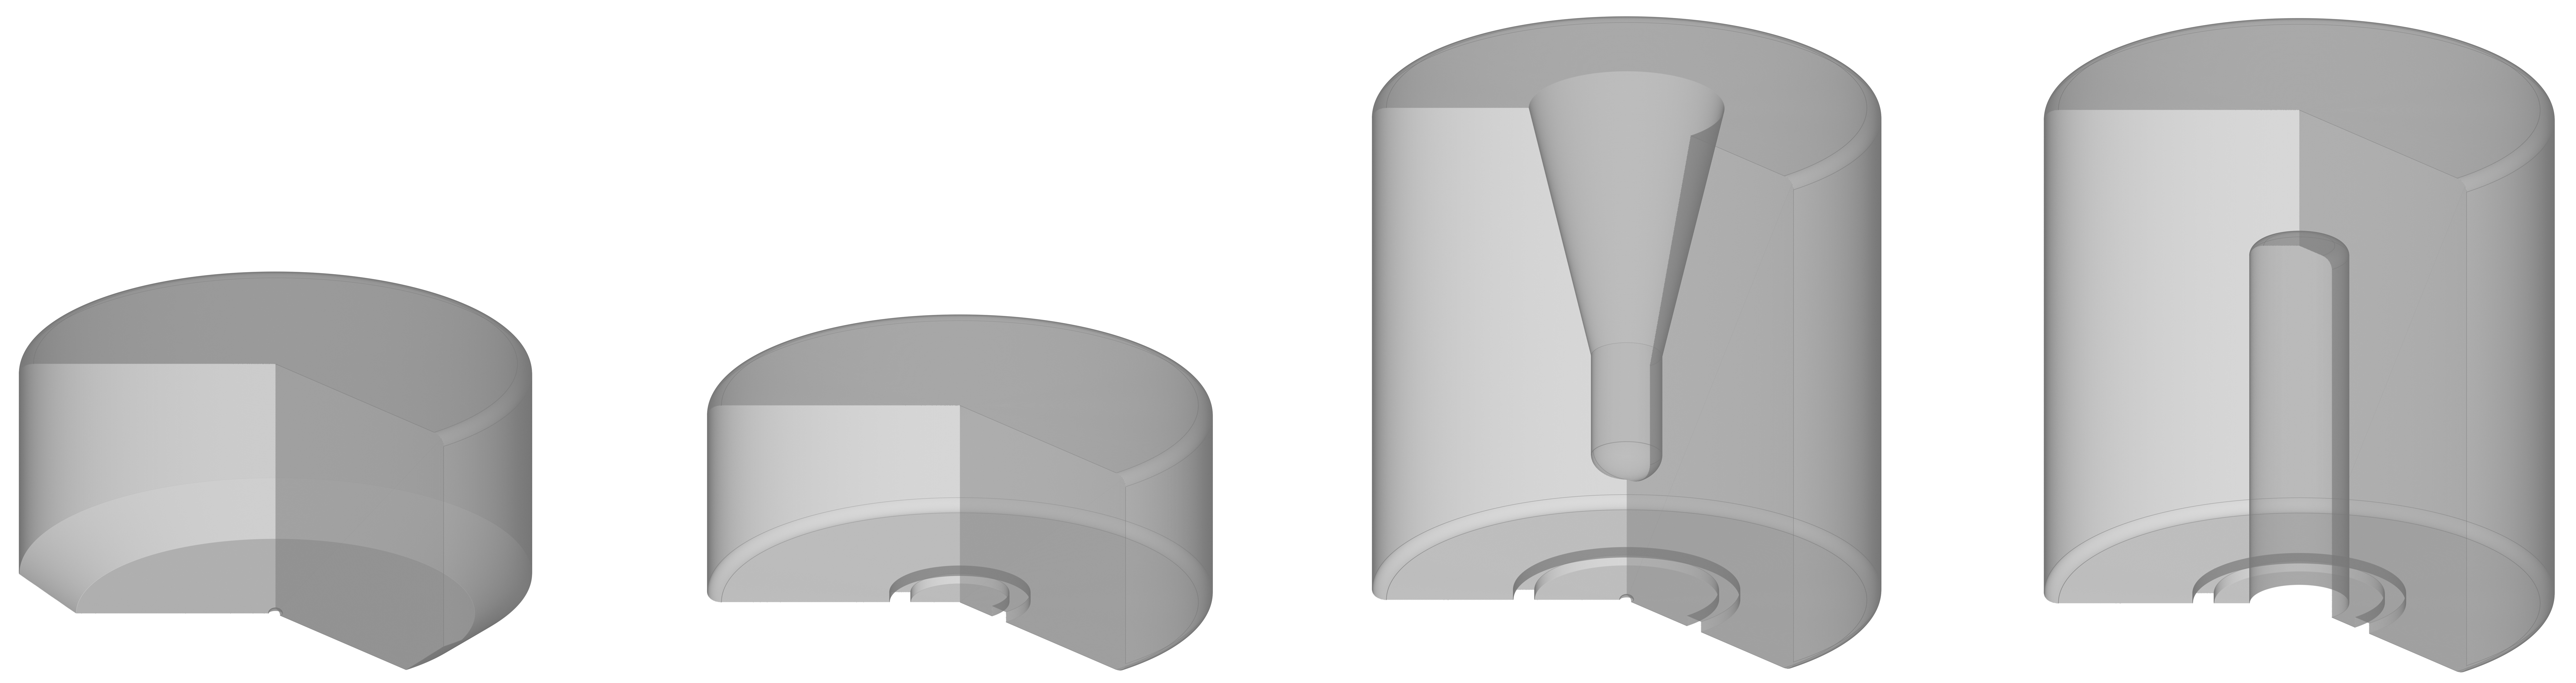
\includegraphics[width=6in]{figs/ge/detectors.png}
	\caption{PPC, ICPC, BEGe and semicoaxial bulk geometries.}
	\label{fig:det_geo}
\end{figure}
\begin{figure}[H]
	\centering
	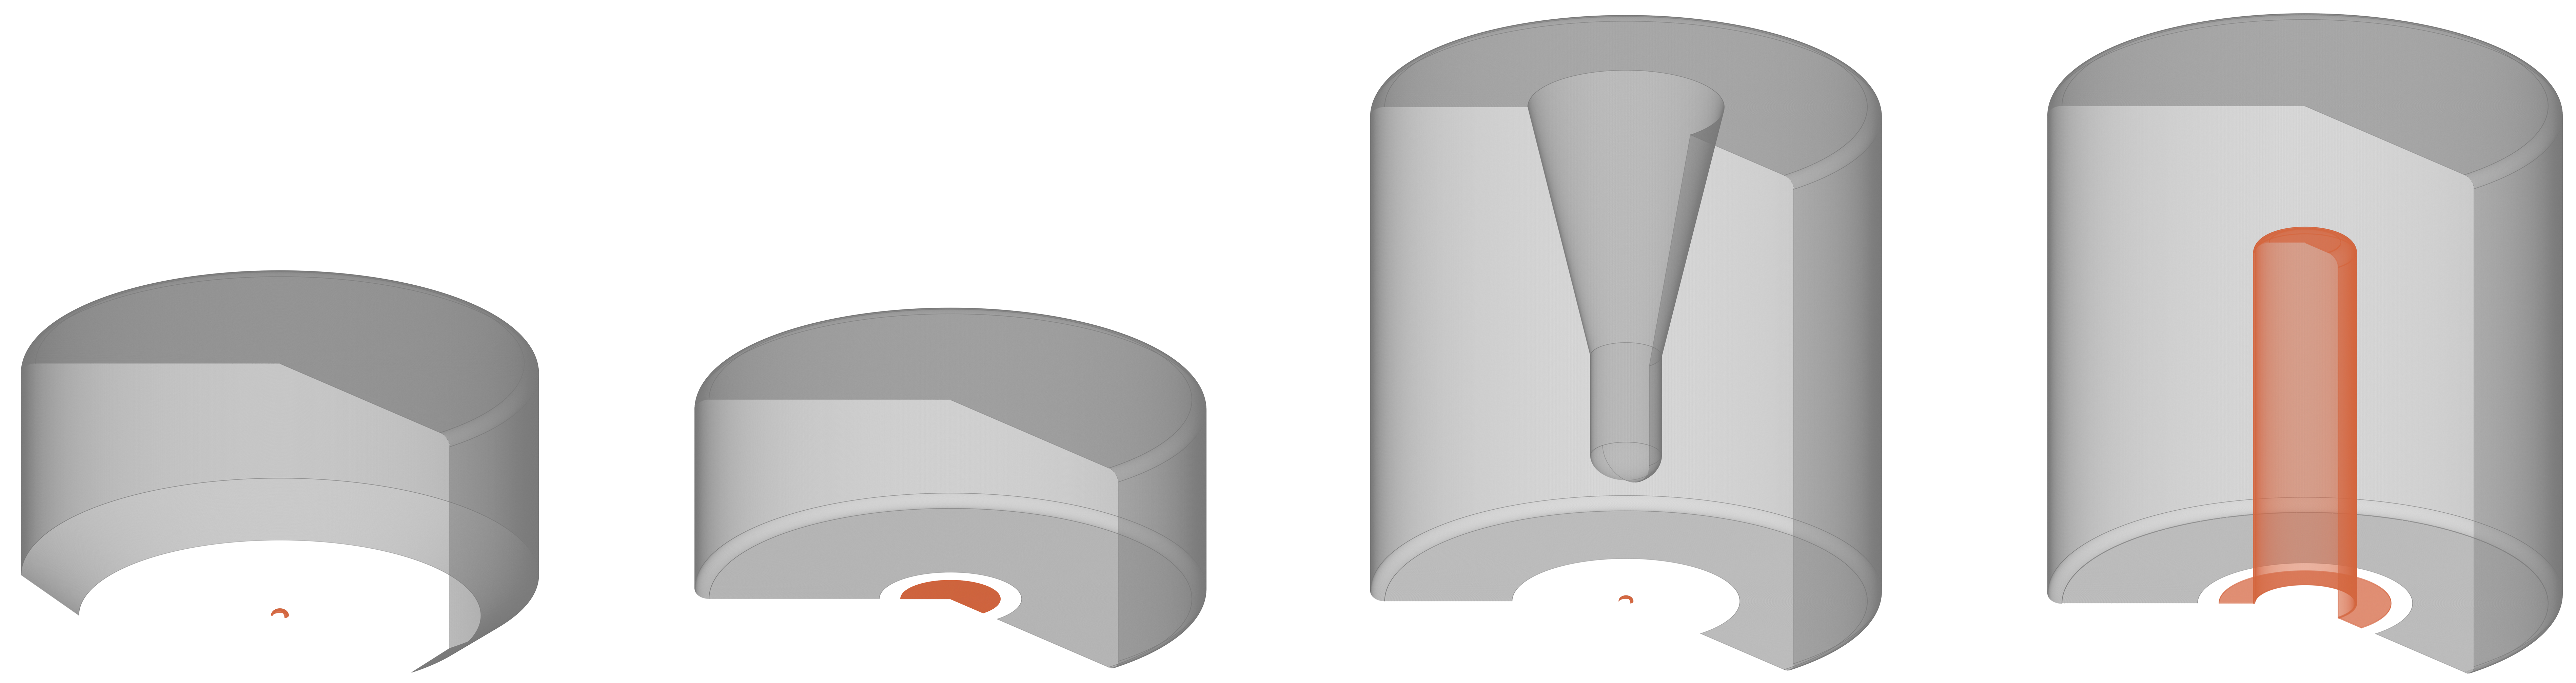
\includegraphics[width=6in]{figs/ge/contacts.png}
	\caption{PPC, ICPC, BEGe and semicoaxial contact geometries. The p$^+$ and n$^+$ contacts are depicted in orange and gray respectively. The surfaces depicted as empty are passivated.}
	\label{fig:det_contacts}
\end{figure}
\begin{figure}[H]
	\centering
	\subfigure[Electric field]{
		\centering
		\includegraphics[width = 2.9in]{figs/ge/e_field.png}
		\label{fig:dets_efield}
	}
	\subfigure[Weighting field]{
		\centering
		\includegraphics[width = 2.9in]{figs/ge/w_field.png}
		\label{fig:dets_weighting}
	}
	\caption{Electric and weighting fields of PPC, ICPC, BEGe and semicoaxial (from top to bottom) HPGe detectors. All detectors are biased 500\,V above the depletion voltage. Six contour lines are plotted for the weighting potential, corresponding to values given by $10^n$ where $n$ varies between -3.5 to -0.5 in steps of 0.5.} 
	\label{fig:dets_fields}
\end{figure}

\section{Energy Resolution}

To obtain a good energy resolution, the measured induced charge does not have to exactly match the charge created at event onset. Rather it just has to be consistent -- the induced charge should be the same for all events where the same charge was created. There are two stages where this consistency breaks down: charge collection and data acquisition. The first is discussed in Section~\ref{sec:charge_trapping}, where the amount of trapped charge varies on an event-by-event basis. The deviation in collected charge is proportional to the induced charge and cannot be fully eliminated by charge trapping corrections. The second is tied to the electronic noise introduced by the instrumentation required to amplify and record the signals. As discussed, detectors with large capacitance amplify this effect.

Of particular concern is low frequency noise, that is, noise with periods of the order or longer than the drift time. Although noise can be averaged or smoothed out, it comes at the cost of timing resolution. The result is that the timing resolution becomes limited to the period of the noise, rather than to the sampling period of the data acquisition apparatus. Thus, smoothing techniques are only applied to correct for high-frequency noise. If timing resolution is not a concern, such as in energy estimation, averaging over periods longer than the drift time through the use of filters is beneficial, and counteracts the effects of noise to an extent. Note that the effects of noise with periods longer than that of a recorded pulse can not be corrected with this method. The amplitude of the noise depends on the electronics circuit -- in which the detector plays the part of a capacitive element -- as a whole and is independent of the induced charge.

In the absence of noise and charge trapping the resolution of the detector is limited by the statistical nature of electron-hole pair production. Given a deposited energy $E_\text{dep}$, the ionization yield or number of electron-hole pairs created along track is $N = E_\text{dep}/\epsilon$. Recall that $\epsilon = 2.96$\,eV per electron-hole pair in Ge. If the number of impacts in the track were governed by a Poissonian distribution, the variance of the ionization yield -- \text{Var}(N)-- would be exactly $N$. Nevertheless, the variance measured by experiment is consistently lower than this value, leading to the conclusion that the events along the track are not independent. The Fano factor~\cite{fano}, $F$, accounts for the deviation from the Poisson predicted variance: $\text{Var}(N) = FE_\text{dep}/\epsilon$. The variance in the measured energy, E, is thus $\text{Var}(E) = \text{Var}(\epsilon N) = \epsilon^2\text{Var}(N) = F\epsilon E_\text{dep}$. In Ge the Fano factor was experimentally determined to be $F = 0.129 \pm 0.003$ at 77\,K~\cite{fanoGe}; however, considerable variation exists in literature. 

Summing the variance from the three effects described above, the resolution of a Ge detector can be parametrized by:
\begin{equation}
	\sigma(E) = \sqrt{\sigma_n^2 + \sigma_F^2E + \sigma_q^2E^2}~,
	\label{eq:energy_resolution}
\end{equation}
where $\sigma_n^2$ accounts for electronics noise, $\sigma_F^2E$ accounts for ionization yield statistics, including the Fano factor, and $\sigma_q^2E^2$ accounts for residual charge trapping. Note that $\sigma_F^2$ is left as a free parameter as opposed to explicitly using $F\epsilon$. This allows to account for energy calibration effects which relates $E$ to $E_\text{dep}$. 

In a hypothetical experiment which measures the ionization yield directly, the relative energy resolution is simply $\sigma/E = \sqrt{F\epsilon}$. Experiments using a wide range of detector technologies have been able to achieve energy resolutions which are dominated by this term, pointing to low noise and good ionization product collection. In this respect, Ge has a considerable advantage, given its comparably low Fano factor and high ionization yield (low $\epsilon$). In combination with its unprecedented high purity, low noise, well understood charge collection properties and modest active volume, the superb energy resolution of HPGe detectors makes them a great tool in the search for new physics.


\chapter{Neutrinoless Double-Beta Decay} \label{chap:theory} 
\section{The ``Little Neutral'' One}
The neutrino, the most elusive of all known fundamental particles, has a lot to say about ``life, the universe, and everything''~\cite{42}. In the 1920s, nuclear beta decay -- the process by which a neutron bound in a nucleus spontaneously decays into a proton by emitting an electron ($n\rightarrow p + e$) -- had thrown the field of physics into an uproar. The electron only carried a variable fraction of the surplus mass-energy of the decaying parent nucleus. This shocking revelation brought into question one of the most fundamental tenets of physics -- the law of conservation of energy. The theoretical physicist, Wolfgang Pauli, proposed that the missing energy was carried away by a yet undiscovered neutral and weakly-interacting particle, the neutrino: a ``desperate remedy'' he called it~\cite{pauli_letter}. Therefore, the beta-decay reaction actually results in a proton, electron, and an antineutrino ($\bar{\nu}$) -- the antimatter counterpart of the neutrino: $$n\rightarrow p + e + \bar{\nu}$$ ``I have done a terrible thing,'' Pauli lamented, ``I have postulated a particle that cannot be detected.''~\cite{pauli_quote} Eventually experimental physicists Frederick Reines and Clyde Cowan proved Pauli wrong nearly 30 years later~\cite{neutrino_discovery}. Thus, the age of experimental neutrino physics began, and physicists became experts at detecting vanishingly rare events with increasingly big detectors. 

\section{Ghosted by the Ghost Particle}
Double-Beta decay (\twovbb{}) is a second order electroweak process and, thus, much rarer than the well known single-beta decay. Single-beta decay is not energetically allowed in certain even-even nuclei; however, in such nuclei \twovbb{} can be observed. Two beta decays occur simultaneously, resulting in the emission of two electrons and two electron anti-neutrinos. It took 52 years from when Maria Goeppert-Mayer first postulated \twovbb{} in 1935~\cite{2vbb}, until it was first observed in $^{82}\text{Se}$~\cite{2vbb_obs}. Then again, the half-life of this isotope is over 9 orders of magnitude above the age of the universe.  This process has now been observed in various naturally existing isotopes with half-lives above $10^{18}$ years. In addition, a related process, double-electron capture, was recently observed by the XENON1T collaboration in $^{124}\text{Xe}$. This is the rarest decay ever observed, with a half-life of $1.8\times10^{22}$ years~\cite{ee_cap}.

The observation of even rarer decays is now within grasp with advances in low background measurement techniques. If neutrinos are Majorana particles, an even rarer event -- neutrinoless double-beta decay (\novbb{}) -- can occur. As opposed to \twovbb{}, no anti-neutrinos would be emitted, thus violating lepton number conservation~\cite{0vbb_theory}. Here, the two electrons carry away all the energy of the decay, producing a peak at the end of the broad \twovbb{} summed electron energy spectrum. This mono-energetic peak is the key experimental signature of \novbb{}. Via light Majorana neutrino exchange, the anti-neutrinos are exchanged as a virtual particle in the nucleus. More exotic mechanisms for \novbb{} have been proposed; nevertheless, regardless of the mechanism, the observation of such a phenomenon would imply that neutrinos are Majorana particles, and as such, they constitute their own anti-particles~\cite{valletheo}. From this point in the text forward, light Majorana neutrino exchange is assumed as the underlying process driving \novbb{}.

In 1937, Wendel Furry invoked Ettore Majorana's theory to propose \novbb{} as alternate mode for $\beta\beta$ decay. Since parity conservation was assumed, Furry postulated that \novbb{} would proceed at a much higher rate than \twovbb{}~\cite{wendell}. However, the opposite has been observed. Even though the leptonic phase space factor for \novbb{}, $G_{0\nu}$, is about 5 orders of magnitude greater than for \twovbb{}, its rate, $(T^{0\nu}_{1/2})^{-1}$, is greatly suppressed by a Majorana mass term, \mbb, such that
\begin{equation}
(T^{0\nu}_{1/2})^{-1} = G_{0\nu}(Q_{\beta\beta},Z)|M_{0\nu}|^2\left(\frac{\langle m_{\beta\beta} \rangle}{m_e}\right)^2~,
\label{eq:rate}
\end{equation}
where $Q_{\beta\beta}$ is the $Q$-value of the decay, $m_e$ is the electron mass, and $M_{0\nu}$ the dimensionless nuclear matrix element (NME) for the decay~\cite{Engel_2017}. The rate is the only observable; thus, $G_{0\nu}$ and the NME must be calculated to extract \mbb{}. If \novbb{} is observed, the knowledge of these factors would contribute to the determination of the underlying model for lepton number violation. Phase space factors depend on the $Q_{\beta\beta}$, the number of particles and the charge of the final state nucleus, $Z$, and have been recently re-calculated to greater precision~\cite{phasespace,phasespace2}. In contrast with the well known, $G_{0\nu}$, NME values for the same isotope differ in factors of 2 -- 3 from each other depending on the model used. When these models are applied to \twovbb{}, the predicted rates are always higher than those measured experimentally. Thus, the calculated NMEs are too large~\cite{jouniga}. The standard remedy is to introduce a quenching factor on the axial coupling constant, $g_A$, which differs for each NME and thus adds to the NME's uncertainty. However, more robust NME models can reduce quenching as shown in a recent publication~\cite{reduced_quenching}. 

Rapid progress in \textit{ab-initio} approaches will soon allow for a more precise computation of these matrix elements and set uncertainties for each one \cite{Engel_2017}. Although \textit{ab-initio} calculations were originally limited to very light nuclei, the NME for $^{48}$Ca has been very recently calculated in this framework~\cite{ca48}. In this respect, the relatively low atomic number of $^{48}$Ca and \geEn{} constitutes an advantage over other \novbb{} candidates. This poses an exciting scenario for the search for \novbb{}. As many tonne-scale experiments are entering their R\&D phase, improved calculations of matrix elements will inform these searches and ultimately allow for the extraction of \mbb{}, if \novbb{} is observed. The uncertainties in the current NMEs highlight the need for a multi-isotope \novbb{} experimental program to determine the effective Majorana mass. Additionally, if a peak is observed at \Qbb{} in one isotope there is the possibility that it could originate from an unknown background. However, if the \Qbb{} peak is observed across multiple isotopes, a strong claim can be made about the discovery of \novbb{}. 

Although neutrinos were long believed to be massless, neutrino oscillation experiments have shown that at least two of the neutrino mass eigenstates have non-zero mass~\cite{osc_sol,osc_atm}. The Pontecorvo-Maki-Nakagawa-Sakata (PMNS) matrix describes the mixing of neutrino mass eigenstates, as governed by three experimentally determined mixing angles. These angles have been observed to be large in comparison to their analogues in quark sector \cite{pdg_revparticlephys}. The superposition of mass states, dictated by the PMNS matrix, leads to the oscillation of neutrinos between different flavor states when these propagate through space. Neutrino oscillations in vacuum are only sensitive to the absolute value of the neutrino mass differences, $\Delta m^2_{ij} = m^2_i - m^2_j$, thus propagation through matter must be leveraged to determine not only the spacing between neutrino mass eigenstates but their ordering. This has been done for neutrinos that travel through the Sun, thus determining $\Delta m^2_{12}$. However, experiments are not yet sensitive enough to determine the sign of $\Delta m^2_{23}$ from neutrinos that are created in the atmosphere as products from cosmic rays, and only $|\Delta m^2_{23}|$ is known \cite{osc_rev}. Thus, the neutrino mass ordering remains partially ambiguous, leading to two possible scenarios, the so-called normal and inverted orderings (NO and IO respectively). Recent global fits of neutrino oscillation parameters moderately favor the NO over the IO at $2.7\sigma$, based on neutrino oscillation data~\cite{NH}. 

The effective Majorana mass, \mbb, depends on elements of the PMNS matrix, $U_{ej}$, and on the neutrino mass eigenstates, $m_j$, 
\begin{equation}
\langle m_{\beta\beta} \rangle = \left|U_{e1}^2 m_1 + U_{e2}^2 e^{i\alpha_{21}} m_2 + U_{e3}^2 e^{i\alpha_{31}} m_3 \right|~,
\label{eq:mbb}
\end{equation}
where $\alpha_{12}$ and $\alpha_{31}$ are two Majorana phases which are allowed if the neutrino is a Majorana particle~\cite{disc_prob0vbb}. Eq.~\ref{eq:mbb} can be rewritten in terms of the lightest neutrino mass $m_l$. The two possible mass orderings would therefore cause the two resulting expressions to diverge from each other if $m^2_l$ is of the order of $\Delta m^2_{ij}$, namely below $10^{-2}$ eV$^2$. The allowed values of \mbb~can be converted into a \Thalf~range via Eq.~\ref{eq:rate}. Applying the current limits given by direct mass measurements (sensitive to $m^2_{\nu_e} = \sum_{i}|U_{e1}|^2m^2_i$) and \novbb{} experiments, and the range of NMEs, gives \Thalf~ $ > 10^{26}$ years.  For the IO, \Thalf~cannot exceed $\sim 10^{28}$ years. The presence of the Majorana phases present a troubling scenario for the observation of \novbb{}. A careful tuning of these parameters in the NO expression would drive \mbb{}, and thus the \novbb{} rate, to zero. However, this scenario is unlikely as shown in a recent global fit which combines oscillation parameter data with limits from \novbb{} experiments and direct mass measurements (See Fig.~\ref{fig:globalfits}).
\begin{figure}[htb]
	\centering
	\includegraphics[width=1\linewidth]{figs/0vbb/globalfits}
	\caption{Marginalized posterior distributions for \mbb~and $m_l$ for the NO (a) and IO (b) assuming the absence of mechanisms that drive $m_l$ or \mbb~to zero~\cite{disc_prob0vbb}. The solid lines denote the region allowed by Eq.~\ref{eq:mbb} assuming 3$\sigma$ intervals of the neutrino oscillation parameters from Ref.~\cite{nufit}.}
	\label{fig:globalfits}
\end{figure}
This global fit predates the newest results from the KATRIN experiment, which cuts the previous limit on $m_{\nu_e}$ in half \cite{katrin, troitsk}. This new limit constrains the parameter space in Fig.~\ref{fig:globalfits} from the right, thus pushing \Thalf~down, slightly disfavoring the quasi-degenerate region. 

The extremely long half--lives involved in \novbb{} present a tremendous experimental challenge; however, the time is ripe for tonne scale experiments to tackle this immense undertaking. The observation of \novbb{} would shed light on many of the fundamental questions in the field, including lepton number conservation, absolute neutrino mass, matter-antimatter asymmetry in the universe, and the nature of the neutrino itself. 

\section{Detecting Vanishingly Rare Events With Increasingly Big Detectors}

How does the \mbb{} parameter space inform the design of an experiment? Using Eq.~\ref{eq:rate} and assuming the neutrino is a Majorana particle with a \mbb{} that lies on the lower edge of the IO region, the corresponding half-life -- assuming the worst case NME -- is of the order of $10^{28}$ years. To design an experiment \textit{sensitive} to this half-life, half-life itself must be understood. In an ideal background free experiment, $N$ atoms are observed for a time $T$. In this experiment, all $D$ decays are detected. From radioactive decay theory $T_{1/2}$ is calculated as,
\begin{equation}
	T_{1/2} = \frac{\ln(2)}{k} 
\end{equation}
and the decay constant, $k$, can be determined from
\begin{equation}
	N - D = N\text{e}^{-kT}
\end{equation}
and approximated as $k = -\ln(1 - D/N)/T \approx D/(NT)$ when $D/N << 1$. Thus, for any rare decay search the half-life can be expressed as
\begin{equation}
	T_{1/2} = \ln(2)\frac{NT}{D} 
	\label{eq:Thalftheo}
\end{equation}

It maybe be that no decays are observed. This non-observation still provides valuable information. As will be seen, a limit on the half-life can be set. Eq.~\ref{eq:Thalftheo} requires some work when applied to a non-ideal experiment where background is present -- such as a \novbb{} search.  ``The sensitivity of an experiment to discover a signal is here defined as the value of \Thalf{} or \mbb{} for which the experiment has a 50\% chance to measure a signal with a significance of at least 3$\sigma$''~\cite{disc_prob0vbb}. This discovery sensitivity, $S^{0\nu(disc)}_{1/2}$, of an \novbb{} experiment is given by
\begin{equation}
	S^{0\nu(disc)}_{1/2} = \ln(2)\frac{N_{\beta\beta}T\epsilon_{tot}\epsilon_{res}}{S}~,
\label{eq:Thalfexp}
\end{equation}

where $T$ is the live time of the experiment, $N_{\beta\beta}$ is the number of \novbb{} candidate nuclei, and $\epsilon_{tot}$, $\epsilon_{res}$, correspond to the total and resolution efficiencies. Understanding the factors in Eq.~\ref{eq:Thalfexp} will allow the savvy experimenter to design an experiment sensitive to \novbb{} half--lives of the desired order. 

The efficiencies in Eq.~\ref{eq:Thalfexp} are included because not all signal events can be detected. Some signal events are discarded by the experimenter's analysis cuts. These are designed to maximize background rejection and minimize the sacrifice of signal events, $1 - \epsilon_{cut}$. Another signal-loss mechanism is of geometric origin. By constructing the detectors from the source material -- the \novbb{} isotope -- the vast majority of signal events are contained within the detector. However, the electrons produced in \novbb{} can escape or be absorbed in the dead layer of the detector. The containment efficiency ($\epsilon_{cont}$) -- the fraction of signal events that are contained in the active volume of the detector -- accounts for this. The total efficiency is given by: $\epsilon_{tot}=\epsilon_{cut}\epsilon_{cont}$.

$S$ now obtains a probabilistic nature as opposed to the previously known and idealized number of signal decays, $D$. $S$ denotes the number of signal events in the \novbb{} region of interest (ROI) for which a 50\% of experiments would report a fluctuation above background with a significance of at least 3$\sigma$. This statement requires some unpacking. Signal events will have an energy of \Qbb{}, however, the finite resolution of the experiment will force the experimenter to define a region of interest around this value to conduct the search.  Note that as the width of the ROI ($\Delta_{\text{ROI}}$) increases, the number of signal events contained in the region increases as well, this fraction is the aforementioned resolution efficiency. Assuming a Gaussian \novbb{} peak, the resolution efficiency takes the following form: $\epsilon_{res} = \text{erf}(\Delta_{\text{ROI}}/(2\sqrt2\sigma_E))$.  Here $\sigma_E$ is the energy resolution of the experiment. Therefore, $\epsilon_{res}$ will increase monotonically with the width of the ROI. However, a wider ROI will include more background counts and will thus increase $S$. Therefore, a savvy experimenter will maximize the figure of merit $\epsilon_{res}(\Delta_{\text{ROI}})/S(\Delta_{\text{ROI}})$ to set the ROI.

To calculate $S(\Delta_{\text{ROI}})$ the number of expected background counts in the ROI, $B$, must be known. A background estimation window (BEW) is used to derive this. In this energy window surrounding \Qbb{}, the background rate (also referred to as the background index), $\mu_b$, is calculated from the number of events in the BEW. These counts are normalized by the width of the BEW and the exposure of the experiment, $MT$, to produce a figure in units of c/(keV\,kg\,yr). The mass of the detector(s) is given by $M =  m_aN_{\beta\beta}/(\eta N_A)$, where $m_a$ is molar mass of the candidate isotope and $\eta$ the isotopic purity. The background rate, $\mu_b$, is assumed constant over the BEW to project $B = \mu_bMT\Delta_{\text{ROI}}$ background counts in the ROI.

$S$ is calculated as follows using the Poisson distribution, $p(n|\nu)$.
\begin{equation}
	\int_{0}^{C}p(n|B)dn = \alpha
	\label{eq:alpha}
\end{equation}
$\alpha$ corresponds the aforementioned significance level of 3$\sigma$ and is thus given by $\alpha = \text{erf}(3/\sqrt{2})$. Eq.~\ref{eq:alpha} uniquely determines the total number of counts in the ROI, C, which is used to solve for $S$ in Eq.~\ref{eq:beta}.
\begin{equation}
	\int_{0}^{C}p(n|B+S)dn = 1-\beta
	\label{eq:beta}
\end{equation}
$\beta = 0.5$ is set from the requirement that 50\% of experiments need to report a fluctuation above background. $S$ is calculated numerically, however, it is of interest to explore the following regimes. In the low background limit, $B<<1$, $S$ is constant, and thus $S^{0\nu(disc)}_{1/2}$ scales linearly with the exposure, $MT$. Note that $N_{\beta\beta}T$ can be replaced by $MT$ along with the appropriate constants in Eq.~\ref{eq:Thalfexp}. Conversely, with appreciable background, $S$ scales with the significance level times the square root of the number of background counts: $S \approx 3 \sqrt B = 3\sqrt{2n\sigma_E\mu_bMT}$. Thus, $S^{0\nu(disc)}_{1/2}$ scales as $\sqrt{MT}$. This finding highlights the importance of minimizing the background so that increases in exposure (which drive the cost of the experiment) can be fully effective. Strictly speaking, an experiment is not background free until $S$ is constant in relation to $B$. However, when there is a high chance of no counts occurring in the ROI, an experiment is considered to be quasi-background-free. 

To reach the required background levels and near unity detection efficiencies, the bulk of the detector must be made of the isotope in question. Many viable technologies exist, including noble gas time projection chambers (TPC), scintillating bolometers, and semiconductor diode detectors. A few general desirable properties of \novbb{} candidates are listed below, most of which can be deduced from Eq.~\ref{eq:rate} and Eq.~\ref{eq:Thalfexp}.
\begin{enumerate}[nolistsep]
	\item High natural abundance and isotope availability,  known enrichment process, and low cost maximizes the exposure, $MT$.
	\item Good energy resolution results in a narrow ROI, reducing backgrounds, and increasing $\epsilon_{res}$. 
	\item $Q_{\beta\beta}$ above the natural background $\gamma$ radiation threshold of 2615 keV. Any radiation above $Q_{\beta\beta}$ can result in energy depositions in the ROI by losing energy in matter interactions.
	\item High intrinsic radiopurity, lowers backgrounds. 
	\item Low \twovbb{} rate $(T^{2\nu}_{1/2})^{-1}$. Although high \twovbb{} rates in the ROI can be strongly suppressed with good energy resolution.
	\item Favorable NMEs and decay phase space factor.
	\item Low atomic number. The  isotope will be at the forefront of \textit{ab-initio} NME calculations.
	\item Well-developed detector technology.
	\item High density. The electrons are contained in smaller volumes and self-shielding is increased.
\end{enumerate} 

Monolithic TPCs can achieve high exposures and have some of the best limit setting capabilities in the field~\cite{exo200}. However, they suffer from modest energy resolution, degrading their discovery level sensitivity. As exemplified by Fig.~\ref{fig:sensitivity_comp}, in the low background regime, modest energy resolution will greatly suppress $S^{0\nu(disc)}_{1/2}$, while reducing the limit setting sensitivity to a lesser extent. In this respect, Ge detector based experiments have an advantage. Furthermore, they can be deployed in a phased approach, as opposed to TPCs, which once built cannot be made larger.

\geEn{} has long been at the forefront of the search for \novbb{}. The decay in question and Q-value are shown in Eq.~\ref{eq:ge76decay}.
\begin{equation}
	^{76}\text{Ge} \longrightarrow ^{76}\text{Se} + 2e^-,~Q_{\beta\beta} = 2039\text{\,keV}
	\label{eq:ge76decay}
\end{equation}
Ge detectors have long been a standard in the field of nuclear and particle physics and are very well posed for this search. The technology has set some of the best limits on \Thalf~to date~\cite{gerda,mjd_final}. As semiconductor diode detectors, their excellent energy resolution constitutes a major advantage. Additionally, the purification of Ge has been carried out further than any element on Earth~\cite{knoll}. Ge has a well-developed enrichment process, and can be readily enriched to 92\% \geEn{}. 

\section{A Hypothetical Tonne-Scale Experiment}\label{sec:design}

Now that all the factors of Eq.~\ref{eq:Thalfexp} are understood, a hypothetical experiment with discovery level sensitivity to a \novbb{} half-life of $10^{28}$ years can be designed. As a starting point, current low background technology is assumed. In particular, the {\MJDEMit}, a \geEn{}-based experiment, is used as a reference. The following performance parameters achieved by the {\DEMit} are used for the calculations below: $\mu_b = 6.6 \times 10^{-3}$\,c/(keV\,kg\,yr), FWHM$_E$ = 2.52\,keV, and $\Delta_\text{ROI}$ = 4.14\,keV~\cite{mjd_26,mjd_final}.

The exposure of the hypothetical experiment is chosen to be 10\,tonne\,yr, for example with 1\,tonne of pure \geEn{} detectors operating for 10 years. With this exposure, $B < 0.0027$ counts is required for the experiment to be truly background free (constant $S$). Nevertheless, applying the performance parameters listed above projects $B = 232$ background counts in the ROI. The value of $S$ for which 50\% of such hypothetical experiments would report a fluctuation above 3$\sigma$ is $S \approx 3\sqrt B =  46$. Plugging these values into Eq.~\ref{eq:Thalfexp} yields a discovery level sensitivity of $S^{0\nu(disc)}_{1/2} = 1.7 \times 10^{27}$ years. Therefore, even with the ultra-low background levels of the {\DEMit}, the $10^{28}$ level of sensitivity is not reached in the tonne-scale hypothetical experiment. The discovery level sensitivity varies with the energy resolution and the background rate as shown in Fig.~\ref{fig:sensitivity_disc}. In this parameter space, the yellow area represents the true background free level. Meanwhile, the hypothetical experiment lies in the lower right-hand edge of the plot. 
\begin{figure}[htb]
	\centering
	\includegraphics[width=6in]{figs/0vbb/discovery_sensitivity.png}
	\caption{Discovery level sensitivity, $S^{0\nu(disc)}_{1/2}$, for a 1 tonne \geEn{} experiment with 10 year live time, as it varies with respect to the background rate and and the energy resolution of the experiment. Assumes 100\% enrichment and $\epsilon_{tot} = 0.8$. In addition to the uniform background rate, contamination from the \twovbb{} is also considered. It is calculated as $B^{2\nu}= (T^{0\nu}_{1/2} S/T^{2\nu}_{1/2})( \sigma_E/Q_{\beta\beta})^6$ \cite{2vbb_background}. Note that this effect is almost negligible -- up to $\mathcal{O}(10^{-7})$ -- in this energy resolution range. ROI optimization is used. Background rate ranges from background free levels to that of the {\MJDEMit}. Energy resolution range is representative of many \novbb{} experiments. Code at \url{https://github.com/hervasa2/sensitivity.git}}
	\label{fig:sensitivity_disc}
\end{figure}

All, however, is not lost. The experiment can run longer or with increased the isotope mass. Unfortunately, this would produce diminishing returns as stated in the discussion of the behavior of $S$ and as seen in the right panel of Fig.~\ref{fig:legend_sensitivity}.  
\begin{figure}[htb]
	\centering
	\includegraphics[width=6in]{figs/legend/legend_sensitivity.pdf}
	\caption{``The sensitivity to a \novbb{} decay signal in \geEn{} as a function of exposure and background for a (left) 90\% CL exclusion sensitivity and (right) 3$\sigma$ (99.7\% CL) discovery sensitivity (DS). Note, the background rates are normalized to a 2.5\,keV FWHM energy resolution.''~\cite{legend_pcdr}}
	\label{fig:legend_sensitivity}
\end{figure}
The hypothetical experiment has a background rate close to that of the dotted blue line in the figure. Nevertheless, a 700-fold reduction in background puts it on the same order as the dashed red line in the figure. This reduction of background rate to $\mu_b = 1 \times 10^{-5}$ c/(keV\,kg\,yr) (B = 0.3), yields $S = 4$, giving the desired $10^{28}$ discovery level sensitivity.

These are exactly the main design requirements for the next generation \novbb{} \geEn{} experiment, LEGEND-1000~\cite{legend}. That is, 10\,tonne\,yr of enriched exposure with a background rate  of $\mu_b < 1 \times 10^{-5}$ c/(keV\,kg\,yr). The drastic reduction in background levels might seem unattainable; however, a reduction factor of 10 has already been demonstrated by the GERDA collaboration~\cite{GERDA2020}. Additionally, in the hypothetical experiment, the effects of scaling up the {\MJDEMit}, were ignored: self-shielding and increased granularity help in background mitigation. For further details on these experiments, refer to Section~\ref{sec:experiments} and Chapter~\ref{chap:legend}.

It very well may be the case that the half-life of \novbb{} is above the design sensitivity: $T^{0\nu}_{1/2} > 10^{28}$. In this scenario, the hypothetical experiment fails to achieve $S = 4$. In the hypothetical situation were 1 count was found in the ROI, the requirement set by Eq.~\ref{eq:alpha} would not be met. In this case, a discovery cannot be claimed, but a limit can be set via
\begin{equation}
T^{0\nu}_{1/2} > \ln(2)\frac{N_{\beta\beta}T\epsilon_{tot}\epsilon_{res}}{UL_{90\%}(B)}~, 
\label{eq:Thalflim}
\end{equation}
where $UL_{90\%}(B)$ is the 90\% confidence level (CL) upper limit on the number of events in the ROI that can be attributed to signal given an expected number of background counts, $B$. A standard way of calculating this is via the Feldman-Cousins approach~\cite{fc}. With $B>5$, the method quickly converges to the standard $UL_{90\%}(B) \propto \sqrt B$. Other methods can be used, such as the extended profile likelihood method used in Ref.~\cite{mjd_26}. Using the Feldman-Cousins method with 1 count in the ROI and 0.3 counts expected from background yields $UL_{90\%}(0.3) = 4$. With such a result the limit $T^{0\nu}_{1/2} > 10^{28}$ is set and therefore the IO ordering region would be excluded under the assumption that the neutrino is a Majorana particle.
\begin{figure}[htb]
	\centering
	\includegraphics{figs/0vbb/gerda_sensitivity.pdf}
	\caption{Historical limits on the \novbb{} half life, \Thalf{} (red), and expected median sensitivity assuming no signal, $S^{0\nu}_{1/2}$ (green), of the GERDA experiment~\cite{GERDA2020}.}
	\label{fig:sensitivity_gerda}
\end{figure}

Experiments in the field not only report a limit, but a median sensitivity, $S^{0\nu}_{1/2}$. To do this, a Monte Carlo simulation of an ensemble of identical experiments is conducted. From this ensemble, the median $UL_{90\%}(B)$,  $\langle UL_{90\%}(B) \rangle$, is extracted. Replacing $UL_{90\%}(B)$ with $\langle UL_{90\%}(B) \rangle$ in Eq. \ref{eq:Thalflim} yields the median sensitivity. As seen in Fig.~\ref{fig:sensitivity_gerda}, the limit, $T^{0\nu}_{1/2}$ -- subject to the statistical variation of counts that appear in the ROI -- fluctuates over the lifetime of the experiment, while $S^{0\nu}_{1/2}$ monotonically increases with the exposure in background free regime of the GERDA experiment.

The median sensitivity varies with the energy resolution and the background rate as shown in Fig.~\ref{fig:sensitivity_heat}. Taking a slice at $\mu_b = 8 \times 10^{-6}$ c/(keV\,kg\,yr) in this figure and in Fig. \ref{fig:sensitivity_disc}, the effect of increasing the energy resolution can be observed. This is shown in Fig.~\ref{fig:sensitivity_comp}, where it is clear that the discovery level sensitivity is suppressed to greater extent than median sensitivity at poorer resolutions. Thus, the superb energy resolution of Ge detectors presents a clear advantage in the search for \novbb{}, with Ge-based experiments having a particularly high discovery level sensitivity.
\begin{figure}[H]
	\centering
	\subfigure[]{
		\centering
		\includegraphics[width=3.7in]{figs/0vbb/median_sensitivity.png}
		\label{fig:sensitivity_heat}
	}
	\subfigure[]{
		\centering
		\includegraphics[width=2.1in]{figs/0vbb/discvslim.png}
		\label{fig:sensitivity_comp}
	}
	\caption{(a) Median sensitivity, $S^{0\nu}_{1/2}$, assuming no signal, for a 1 tonne \geEn{} experiment with 10 year live time, as it varies with respect to the background rate and energy resolution of the experiment. Assumes 100\% enrichment, $\epsilon_{tot} = 0.8$, and \twovbb{} contamination. 1000 identical experiments are simulated in each case. (b) Median sensitivity, assuming no signal (solid black, as calculated from 10,000 identical simulated experiments), and discovery level sensitivity (dashed black) as it varies with energy resolution.} 
	\label{fig:sensitivity}
\end{figure}

\section{Searching for \novbb{} With Germanium Detectors} \label{sec:bg_disc}

In \novbb{}, two electrons carry all the energy available in the decay. Due to the high density of \geEn{}, the range of electrons is limited to 1\,mm. Therefore, a very high percentage of events are fully contained in the bulk, and the energy is deposited within 1\,mm of the decay vertex. Meanwhile, surface events are likely caused by alpha and beta emitters outside the detector. Therefore, large detectors are desirable since they have a lower surface-to-volume ratio. In Ge full event topology cannot be reconstructed, and event selection is fully based on the modeling of pulse-shapes in the detector. However, the inherent single-site topology of \novbb{} events in dense materials allows for a powerful discrimination of backgrounds.

The 0.5 -- 1 mm thick n$^+$ dead region is too thick for alpha particles to transverse and deposit energy in the ROI. The n$^+$ contact extends over the most of the surface of PPCs, BEGes and ICPCs. However, the small fraction not covered provides an entry window for alpha particles. In {\MJMit} style PPCs in particular, a large fraction of the bottom of the detector is covered by a passivated region, which isolates the p$^+$ and n$^+$ contacts. Events occurring on this surface are characterized by incomplete charge collection due to slow charge drift and trapping on the surface. Therefore, alpha events, which have known energy peaks above 5 MeV, can fall in the much lower ROI of \novbb{}.

Charge trapping along the drift path is a potential issue for all events. Events in the bulk of the detector, such as those triggered by gamma particles are subject to this effect. This can be seen in the low energy tails of known gamma peaks. A bulk-charge trapping correction is applied for such events which mitigates the low energy tailing. On the other hand, charge trapping on detector surfaces is not as well understood and a correction cannot be applied. Nevertheless, these events can still be identified and discarded. By conducting scans with alpha sources on the passivated region of PPC detectors, the delayed charge recovery (DCR) effect was observed. A fast pulse with incomplete charge will form in the detector, thus resulting in a degraded energy reading. As the event progresses, charge carriers at the detector surface are released over time, resulting in a positive slope of the charge signal tail. In the {\DEMit}, the DCR parameter was developed to systematically identify and remove these events, resulting in a drastic reduction of surface events falling in the \novbb{} ROI~\cite{dcr}. A careful handling of the detectors and supporting structural materials further aids in the reduction of surface backgrounds. For example, Ge detectors are kept in vacuum or in nitrogen-flushed environments to avoid deposition of the alpha-emitting $^{222}$Rn found in air.
\begin{figure}[htb]
	\centering
	\includegraphics[width = \linewidth]{figs/0vbb/bkg_events.png}
	\caption{Background mitigation strategies. From left to right: illustration of the acceptance of $\beta\beta$ events, rejection of coincident events between two neighboring detectors, rejection of multi-site and surface events and rejection of coincident events between a detector and LAr. p$^+$ contacts are shown in orange~\cite{legend_website_detectors}.} 
	\label{fig:bkg_disc}
\end{figure}

Other surface events include energy depositions in the transition region between the n$^+$ contact and the bulk of the detector. The so-called late charge (LQ) parameter is determined by the ``integral of uncollected charge after a waveform has reached 80\% of its maximum value''~\cite{mjd_final}. Charge carriers produced in this region slowly diffuse to the bulk of the detector, resulting in increased pulse rise times and characteristically high LQ. Finally, p$^+$ contact events are characterized by abnormally fast pulse rise times and thus exhibit a large current amplitude, $A$, with respect to the event energy $E$. By dividing $A$ by $E$ a discriminator against these, and other, events is created -- the $A/E$ parameter. p$^+$ contact events can be removed by a high-$A/E$ cut. 

Events in the bulk of the detector can also originate from backgrounds. Gamma particles can fully transverse the detector; therefore, Compton scatters originating from full energy peaks above \Qbb{} can produce signals in the ROI. Of particular concern are the primordial isotopes $^{232}$Th and $^{238}$U, whose decay chains contain $^{208}$Tl and $^{214}$Bi respectively. The corresponding prominent 2615\,keV and 2204\,keV gamma peaks are well above \Qbb{} and can be observed in the spectra of \geEn{}-based experiments (Fig.~\ref{fig:mjd_spectrum} and Fig.~\ref{fig:gerda_spectrum}). $^{232}$Th and $^{238}$U can be found in virtually all earth-based materials. The fist line of defense against such contaminants is not introducing them in the first place. For this reason, the materials chosen to build \novbb{} experiments, particularly materials close to the detector(s), undergo extensive radiopurity screening and selection.

If a gamma particle scatters and deposits energy in more than one vertex in the detector -- a so-called multi-site event -- the resulting pulses will exhibit an extended multistep current amplitude. The amplitude will be degraded with respect to a single-site event of the same energy. Therefore, multi-site events can be removed by a low $A/E$ cut. The $A/E$, LQ and DCR discriminators are examples of pulse-shape discrimination (PSD) techniques.
\begin{figure}[htb]
	\centering
	\includegraphics[width=6in]{figs/0vbb/sse_mse.pdf}
	\label{fig:mse}
	\caption{A multi-site event (right) presents an extended multistep current amplitude with respect to that of a single-site event (left) of the same total energy and thus rejected. These events are simulated in a PPC detector. The energy deposition locations and drift paths are shown in white and overlaid on the PPC's weighting potential. The outline of the detector is also shown in white.} 
\end{figure}

If gamma particles scatter in a detector and escape, a different approach is needed. Such events can be vetoed via anti-coincidence cuts if they deposit energy in any other active material in the experiment, which could be another Ge detector. In this regard, surrounding the detectors by active material is beneficial. For example, operating the detectors in liquid argon (LAr) provides an active medium which scintillates when struck by Compton scattered gammas. The light can be read out by instrumenting the LAr. However, the LAr itself, which is in contact with the germanium, is a source of additional backgrounds. Therefore, this approach comes at a higher risk when compared to the traditional operation of detectors in vacuum. The {\MJDEMit} and GERDA experiments highlight the difference between these approaches.

\section{Present and Future Experiments} \label{sec:experiments}

The {\MJMit} collaboration searched for \novbb{} in \geEn{} using enriched, high-purity Ge (HPGe) detectors. The {\MJDEMit} consisted of an array of HPGe detectors located in the Sanford Underground Research Facility (SURF) in Lead, South Dakota~\cite{mjd}. The ultra-low background and record energy resolution achieved by the {\DEMit} enabled a sensitive \novbb{} search, as well as additional searches for new exotic physics~\cite{mjd_axions, mjd_trinucleon,mjd_waveform}.
\begin{figure}[htb]
	\centering
	\subfigure[{\MJDEMit}]{
		\centering
		\includegraphics[height = 0.3\linewidth]{figs/0vbb/mjd}
		\label{fig:mjd}
	}
	\subfigure[GERDA]{
		\centering
		\includegraphics[height=0.3\linewidth]{figs/0vbb/gerda}
		\label{fig:gerda}
	}
	\caption{ The {\MJDEMit} (a) and GERDA (b) experiments.} 
	\label{fig:experiments}
\end{figure}

The {\MJDEMit} consisted of two modules with a total of 40.4\,kg of HPGe detectors (27.2 kg enriched to 88\% in \geEn{}) operated in vacuum. Initially, all enriched detectors were of PPC geometry; however, in the final stage of data taking five PPCs were replaced by four ICPC detectors. Both vacuum cryostats and all structural components of the detector arrays were machined from ultra-low-background underground electroformed copper (UGEFCu)~\cite{ugefcu} and low-background plastics. Low-radioactivity Parylene was used to coat UGEFCu threads to prevent galling and for the cryostat seal~\cite{mjd_og}. A layered shield enclosed both modules. The innermost layer consisted of 5\,cm of UGEFCu. Five cm of commercial oxygen-free high conductivity copper (OFHCu) and 45\,cm of high-purity lead followed. The shield and module volume were constantly purged with low-radon liquid nitrogen boil-off gas. The aluminum enclosure that isolated this Rn-excluded region, was covered with a plastic active muon veto which provided near-$4\pi$ coverage~\cite{muonveto}. The near-detector readout system, which was integrally designed for the {\DEMit}, included low-mass front end (LMFE) electronics~\cite{lmfe} and low-mass cables and connectors~\cite{cables}. Cables were guided out of each module following a UGEFCu cross-arm which penetrated the layered shield. The cross-arm connected the cryostat with vacuum and cryogenic hardware. Control and readout electronics were just outside the Rn-excluded region. The entire assembly was surrounded by 5\,cm of borated and 25\,cm of pure polyethylene to shield against neutrons.
\begin{figure}[tbh]
    \centering
    \includegraphics[width=6in]{figs/0vbb/mjd_spectrum.pdf}
    \caption{``The measured energy spectrum above 100\,keV for the [{\MJDEMit}'s] full enriched exposure after applying multiplicity and data cleaning cuts (dark gray), DCR, high-$AvsE$ and LQ cuts (light gray), and the low-$AvsE$ cut (red)''~\cite{mjd_final}}
    \label{fig:mjd_spectrum}
\end{figure}

The {\MJDEMit} applied the discussed DCR, high-LQ and high-and-low-$AvsE$ (similar to $A/E$) cuts to reject backgrounds. After cuts, the {\DEMit} set a lower limit of $T^{0\nu}_{1/2} > 8.3\times10^{25}$ years and reached a sensitivity of $S^{0\nu}_{1/2} = 8.1\times10^{25}$ years, with an exposure of 64.5\,kg\,yr. The corresponding background rate is of $6.6\times10^{-3}$ c/(keV\,kg\,yr)~\cite{mjd_final}. Although the measured background is almost 6 times higher than the assay-based model for the {\DEMit} predicts~\cite{assaypaper}, ongoing background modeling efforts point towards an unaccounted $^{232}$Th excess consistent with a source far away from the detectors. Therefore, critical components near the detectors such as UGEFCu parts and LMFE electronics are safe to use in future experiments. The energy resolution achieved by the {\DEMit} -- 2.52 keV FWHM at \Qbb{} -- is the best of any \novbb{} experiment. The lower limit on the half-life was used to calculate an upper limit on the effective Majorana mass using Eq.~\ref{eq:Thalfexp} and values from literature. Using ``a range of $M_{0\nu}$ values of 2.66-6.34, phase space factors ($G_{0\nu}$) of $2.36\times10^{-15}$ or $2.37\times10^{-15}$, and an effective axial weak coupling of $g^\text{eff}_A=1.27$ for free nucleons''~\cite{mjd_final} gives an upper limit on \mbb{} in the range of 113-269\,meV. In fulfillment of its experimental goals, the {\MJMit} collaboration has demonstrated backgrounds low enough to warrant the construction of a tonne-scale experiment. 
\begin{figure}[tbh]
    \centering
    \includegraphics[width=5in]{figs/0vbb/gerda_mjd_limits.pdf}
    \caption{The limit placed on $\langle m_{\beta\beta} \rangle$ by the {\MJDEMit} is shown as a light gray central band in the $\langle m_{\beta\beta} \rangle$ parameter space. A breakdown of this range into the individual upper limits derived from the relevant nuclear matrix elements found in literature is shown on the right. The broken down limits achieved by GERDA (\geEn{}), KamLAND-Zen ($^{136}$Xe), EXO-200 ($^{136}$Xe) and CUORE ($^{130}$Te) are also included~\cite{mjd_final}.}
    \label{fig:gerda_mjd_limits}
\end{figure}

The Germanium Detector Array (GERDA) collaboration operated an array of \geEn{}-enriched HPGe detectors at Laboratori Nazionali del Gran Sasso (LNGS) in Italy. The detectors used were also of p-type point-contact technology: BEGes and ICPCs. GERDA took a novel approach to background suppression based on a LAr active veto~\cite{lar_veto}.  This is in direct contrast to the tried and true detector-in-vacuum approach of the {\MJDEMit} and others before it, such as the Heidelberg-Moscow and IGEX experiments~\cite{h-m, igex}. The GERDA detector strings were suspended in LAr and surrounded by a shroud of silicon-photomultiplier-coupled wavelength shifting fibers. Background suppression was achieved by anti-coincidence cuts between events read out by Ge detectors and scintillation light collected by the fiber shroud. In addition, also in contrast with the {\DEMit}, GERDA opted for a water Cherenkov muon veto, which encapsulated the LAr cryostat. The GERDA water tank was lined with photomultipliers that read out the Cherenkov light produced when a muon interacted in the water. 

GERDA used a single parameter, $A/E$, to perform all background cuts. In BEGe and ICPC detectors, the passivated surface, is much smaller than in the {\MJMit} PPCs. Given its proximity to the p$^+$ contact, events occurring on this surface can be cut with a high-$A/E$ cut. Additionally, the standard low-$A/E$ cut is used to reject multi-site events. GERDA achieved a lower limit of $T^{0\nu}_{1/2} > 1.8\times10^{26}$ years with an exposure of 103.7\,kg\,yr. The corresponding upper limit on the effective Majorana mass is $\langle m_{\beta\beta} \rangle < 79-180\text{\,meV}$. Fig.~\ref{fig:gerda_mjd_limits} summarizes the best limits set on $\langle m_{\beta\beta} \rangle$ by the {\MJDEMit}, GERDA and other experiments searching for \novbb{} in different isotopes. GERDA's background rate is $5.2\times10^{-4}$ c/(keV\,kg\,yr) -- the lowest of any \novbb{} experiment~\cite{GERDA2020}. This equates to under 1 count in the ROI given the GERDA exposure -- a quasi-background-free level -- and has set the standard for the next generation of experiments.

\begin{figure}[tbh]
    \centering
    \includegraphics[width=6in]{figs/0vbb/geda_spectrum_breakdown.pdf}
    \caption{``GERDA Phase II energy spectra (53.9\,kg\,year). Enriched coaxial and BEGe data are displayed in a combined spectrum after indicated cuts. Main contributions to the spectra are labeled. The insets display the analysis window for coaxial and BEGe detectors separately, including the background rates (solid blue lines). No event reconstructs within $Q_{\beta\beta} \pm 2\sigma$. The dashed blue curves depict the 90\% C.L. limit for a \novbb{} signal of $T^{0\nu}_{1/2} = 0.9\times10^{26}$ years derived from the likelihood analysis of all GERDA datasets.''~\cite{gerda}}
    \label{fig:gerda_spectrum}
\end{figure}  

Fig.~\ref{fig:mjd_spectrum} and Fig.\ref{fig:gerda_spectrum} show the final spectra of the {\DEMit} and a GERDA spectra with similar exposure respectively. The GERDA spectrum demonstrates the self-vetoing power of the instrumented LAr. The LAr introduces $^{42}$K, a daughter of the long-lived $^{42}$Ar found in atmospheric Ar. $^{42}$K undergoes beta decay, and the progeny de-excites resulting in a 1525\,keV gamma line. These gammas and associated Compton scatters are seen in the Ge spectra. If the associated beta particles deposit energy in the LAr, such events can be vetoed by applying the anti-coincidence cut. Note that a prominent $^{42}$K peak is not present in the {\DEMit}'s spectra. The LAr is also particularly effective at eliminating events in the Compton continua of the $^{208}$Tl and $^{214}$Bi peaks, resulting in a strong background suppression in the \novbb{} ROI. This region is dominated by passivated surface events in the spectra of the {\DEMit}. After all cuts, a higher background still remains, which is suspected to originate from the Compton continuum of $^{208}$Tl, indicating the presence of the aforementioned $^{232}$Th contaminant. By comparing the full spectrum before cuts to the prominence of the \twovbb{} spectrum in the GERDA and {\MJDEMit} spectra the effect of running in LAr vs. in vacuum can be observed. A lower background is observed in the {\DEMit} in the (1000-1500)\,keV and > 3000\,keV regions due to the $^{42}$K gammas and $^{42}$K betas and other alpha emitters in GERDA respectively. The {\MJDEMit}'s focus on ultra-low background construction materials and careful handling and tracking of parts is responsible for its low background before cuts. 

It is clear that the experimental strategies of GERDA and the {\MJDEMit} are complimentary and should be combined. Drawing from both experiments, a new collaboration was born. GERDA achieved its experimental design goal of 100\,kg\,yr of exposure, and its infrastructure now houses the first phase of the next generation \novbb{} experiment in \geEn{}: The Large Enriched Germanium Experiment for Neutrinoless Double-Beta Decay (LEGEND-200).

\chapter{LEGEND}\label{chap:legend}

LEGEND used the best technologies, and existing resources, from {\MJMit} and GERDA to deploy a 200 kg detector array in the GERDA cryostat (L200). LEGEND aims to pursue a tonne-scale \geEn{} experiment in the next phase of its experimental program (L1000), with $0\nu\beta\beta$ discovery potential at a half-life approaching or at $10^{28}$ years \cite{LEGEND2021}. 

\section{A Trans-Atlantic Union}

GERDA and {\MJMit} have the lowest and second-lowest background rates and second-best and best energy resolutions of any \novbb{} experiment respectively.

The {\MJDEMit}'s careful study and selection of radiopure construction materials resulted in ultra-low background levels. In particular, {\MJMit}'s development and use of UGEFCu spearheaded this result with specific activities orders below many of the other materials employed~\cite{assaypaper}. Note that most of the mass in proximity of the detectors is UGEFCu. Another low-background component developed by the {\MJMit} collaboration is the LMFE. The LMFE sits next to the p$^+$ contact of each detector and in combination with further electronics upstream, constitutes the preamplifier for each channel. This design places the preamplifier's critical components next to the detector to avoid noise pickup along cables, and moves all the other -- often high activity -- electronics further away. The use of LMFEs was instrumental to the {\DEMit}'s record energy resolution.

By integrating the materials and electronics pioneered by the {\MJMit} collaboration into GERDA-style germanium strings in a LAr veto, the record background rate of GERDA can be surpassed. This is the strategy used by the LEGEND collaboration, driving its discovery potential to \novbb{}. From their onset, the {\MJMit} and GERDA collaborations developed joint analysis and simulation software and shared PSD techniques and Ge detector characterization results. These techniques have matured in the last decade and are ripe for their application to LEGEND data. The combination of ultra low background materials, low-noise front-end electronics, mature PSD techniques, and a LAr veto with an improved light readout system, results in a predicted background rate of $2 \times 10^{-4}$ c/(keV\,kg\,yr) and $9 \times 10^{-6}$ c/(keV\,kg\,yr) for L200 and L1000 respectively~\cite{legend_pcdr}. 

\section{L200}

Using the GERDA water tank and LAr cryostat at LNGS allowed LEGEND to expedite the deployment of a 200\,kg \geEn{} detector array. L200 utilizes the existing 70\,kg of detectors from GERDA and {\MJMit} in addition to 130\,kg of new ICPC detectors. Modifications to the GERDA infrastructure were needed to accommodate the larger L200 array. The Ge detector strings were mounted in between two new fiber optic barrels, designed specifically for the L200 string layout. The new design, in combination with higher-purity LAr, has led to higher light yield, transmission and detection. Each string consists of detector units, varying in number and size depending on the unique geometry of each detector. The detector configuration of each string and the string placement with respect to others has been optimized to increase light collection, detector density (results in more coincident events in neighboring detectors, thus allowing to discriminate against gamma backgrounds), and maintain the balance of the array. 
\begin{figure}[htb]
	\centering
	\includegraphics{figs/legend/detector_unit_width_4in.pdf}
	\caption{Render of the L200 detector unit.}
	\label{fig:legend_detector_unit}
\end{figure}

Each detector unit consists of a Polyethylene naphthalate (PEN) plate supporting three UGEFCu rods and an LMFE garage. PEN is a radiopure scintillating structural plastic~\cite{pen}, thus PEN plates increase light yield and transmission in a region proximal to the detector. The detector sits on three radiopure ultem insulators and is wire bonded to the LMFE garage. A LMFE is docked in the garage and its wires follow the string towards the top copper plate and is connected to a CC4 board, closing the preamplifier circuit. The CC4 board accommodates multiple LMFE connections. Note that this design allows LMFEs to be replaced without disassembling a string. A similar garage houses a HV clip which supplies up to 5000\,V to the detector. The detector units link and hang from one another at the UGEFCu rods forming a string. The strings are enclosed in nylon mini-shrouds. This impedes the drift of $^{42}$K ions outside the shroud volume towards the detector, thus mitigating $^{42}$K beta background in the \novbb{} ROI. However, nylon is opaque to the 128\,nm scintillation light of Ar and therefore the shrouds are coated with wavelength shifting tetra-phenyl-butadiene (TPB). The light is shifted to 450\,nm which is suitable for transmission through the mini shrouds and detection by the LAr veto~\cite{gerda_upgrade}. In similar fashion the optic fibers comprising the inner and outer fiber barrels are coated with TPB. The barrels surround the strings to maximize light collection. In each barrel, the fibers are coupled to silicon photomultipliers (SiPMs) at the top and bottom. 

The Ge array and light readout system is lowered into the center of the LAr cryostat for operation, where it is surrounded by a wavelength shifting reflector. The LAr cryostat is filled with 5N LAr, and its optical properties and thus purity are monitored by the Liquid Argon Monitoring Apparatus (LLAMA)~\cite{llama}. The LAr acts as a cooling medium for the Ge detectors, an active scintillating volume in the near detector region, and a passive high-density radiation shield. Radioactive sources are lowered into the deployed array to perform periodic energy calibrations. The sources are encapsulated and guided through the source guidance funnels and calibration source tubes to multiple locations along the Ge strings.

The LAr cryostat sits in a 8.5\,m high water tank which is filled with 590\,m$^{3}$ of ultra-pure water for operation. The 3500\,m water equivalent overburden in the LNGS underground site results in a muon flux of around $3.5\times10^{-4}$\,m$^{-2}$s$^{-1}$~\cite{lngs_muon_flux}. GERDA measured a muon rate of 0.04\,Hz~\cite{gerda_muon_veto} with the same infrastructure. The Cherenkov light created by the passage of muons in water is read out by PMTs on the walls and floor of the water tank. Coincident events in the Ge and water tank can thus be vetoed. The coincidence window in Ge is expanded to further veto prompt events proceeding a muon interaction. The resulting deadtime acquired highlights the need for a deep underground location.

L200 targets a 1\,tonne\,yr of exposure to reach a 3$\sigma$ \novbb{} discovery sensitivity of 10$^{27}$\,yr. This translates into a \mbb{} upper limit in the range of 34-78\,meV. The target exposure can be reached by operating the 200\,kg array for 5 years. The 130\,kg of new ICPC detectors have an average mass above 2\,kg, approximately twice that of the largest PPCs and BEGe detectors employed. Thus, the number of new detectors needed to reach the target exposure was halved. Fewer detector channels translates into fewer structural materials, cables and electronics in the array, thus resulting in a significant background reduction. These detectors have a lower surface to volume ratio which mitigates surface backgrounds as discussed. The combination of the adoption of {\MJMit}-style low-noise electronics, low-mass and radiopure components, a LAr veto with higher light yield and transmission, and larger detector masses results in a projected $2.5\times$ reduction from GERDA's record background index. L200 has been in a stable data-taking configuration since March 2023.
\begin{figure}[H]
	\centering
	\includegraphics[width=5.4in]{figs/legend/legend_width_6in_rq.png}
	\caption{Render of the full L200 experimental design with a zoom into the Ge payload with light readout system. The front-facing Ge strings and section of the outer fiber barrel are cut out for clarity. The individual water tank and barrel schematics were rendered by Patrick Krause of the LEGEND collaboration.}
	\label{fig:legend_barrel}
\end{figure}

\section{L1000}

In the proposed L1000 experiment, 42 strings -- totaling over 1000\,kg of \geEn{} -- are operated in underground sourced LAr (UGLAr)~\cite{legend_pcdr}. The target average detector mass is 3\,kg. The UGLAr will be sourced from a deep CO$_2$ well and has been demonstrated to contain 1400 times less $^{39}$Ar than atmospheric Ar~\cite{uglar}. $^{39}$Ar and $^{42}$Ar are both produced in atmospheric Ar by cosmogenic activation, thus a similar reduction factor for $^{42}$Ar is expected. This reduction results in a drastic suppression of the $^{42}$K background in L1000 as compared to L200. The strings will be independently deployed in an UGLAr-filled reentrant UGEFCu tube, allowing payloads to be deployed as detectors are manufactured. A large atmospheric LAr cryostat houses the reentrant tube and provides additional passive shielding and light readout. The light readout system in this region is under study with PMT- and SiPM-clad walls being considered.  Similar to L200 and GERDA, the atmospheric LAr cryostat sits in a water muon-veto tank. The light readout system in the L1000 strings is similar to that of L200, but each string will have its own fiber array with improvements in light yield, transmission, and detection. The experimental site is under consideration, with LNGS as the main candidate.
\begin{figure}[htb]
	\centering
	\includegraphics[width=6in]{figs/legend/L1000.png}
	\caption{The conceptual design of the L1000 experiment. Rendered by Patrick Krause.}
	\label{fig:legend1000}
\end{figure}

The detector signal readout sees a major modification from L200. Each Ge detector is wire-bonded to a front-end application-specific integrated circuit (ASIC) board. The low-background ASIC board outputs an amplified signal directly at the detector, as opposed to the approximately 1\,m long LMFE-CC4 loop. The advantage of ASIC-based front electronics is thus two-fold: besides the in-detector-unit pre-amplification, the mass and activity of the near-detector electronics is drastically reduced. Due to the design of L1000, the detector signals have to travel around 10\,m until digitized. Therefore, the use of ASICs is crucial to drive signals this distance with minimal distortion. 

The factor of over 20 reduction in background from L200 to L1000 is driven by the use of UGLAr to reduce the content of $^{42}$K. Meanwhile, the shift to ASIC-readout and the using larger detectors reduces the backgrounds originating from structural components and electronics ($^{232}$Th and $^{238}$U) and from surface alphas. The cosmogenic production of $^{68}$Ge in Ge detectors constitutes a problematic background. It undergoes electron capture to form $^{68}$Ga, which given its Q-value of 2.9\, MeV has a decay spectrum covering the \novbb{} ROI~\cite{mjd_muonic}. $^{68}$Ga decays within the detector, with an event topology that mimics that of \novbb{}; therefore, it is not possible to discriminate against these events. For this reason, the amount of time that the detectors (and raw Ge) spend on the Earth's surface is minimized and carefully monitored. The 271-day half-life of $^{68}$Ge allows for a cool-down in the live-time of the experiment. The principal projected backgrounds of L1000 (before analysis cuts, as compared to GERDA) are outlined in Fig.~\ref{fig:legend_background}. 
\begin{figure}[htb]
	\centering
	\includegraphics[width=6in]{figs/legend/legend_background.pdf}
	\caption{``The expected background index associated with each of the dominant sources, before applying analysis cuts, projected for LEGEND-1000 (blue) and measured in GERDA (red). Significant reductions in all categories, with the exception of internal cosmogenic backgrounds, are predicted based on the use of lower-background materials, Ar extracted from underground deposits, and the use of larger mass detectors.''~\cite{legend_pcdr}}
	\label{fig:legend_background}
\end{figure}

L200 is crucial to the development of the technologies envisioned for L1000. The low-background environment and design of L200 is similar to that of L1000, therefore L200 is a unique test stand to deploy and characterize L1000 technologies. The successive reduction of background and increases in exposure from the {\MJDEMit} and GERDA, to L200, and culminating in L1000 pushes the sensitivity of the LEGEND program beyond the IO region. The target exposure of L1000 -- 10\,tonne\,yr -- is obtained by operating the array for over 10 years from when the first payload is deployed. A 3$\sigma$ \novbb{} discovery sensitivity of L1000 is $1.3\times10^{28}$\,yr is projected which translates into a \mbb{} upper limit in the range of 9-21\,meV.

\section{The Need for ICPC Detectors}

The background requirements of experiments such as L1000 motivated the design of large point-contact detectors. Ge detectors with masses over 2\,kg are routinely used in various applications; however, previous to the development of the ICPC geometry, these detectors were only of the coaxial or semicoaxial geometries introduced in Section~\ref{sec:charge_drift}. In fact, a few semicoaxial detectors were operated in the GERDA array and were carried over to L200. However, such detectors have a higher capacitance than their point-contact counterparts, leading to noisier signals and poorer energy resolution. Additionally, the longitudinal isotropy of the electric field in coaxial detectors leads to a convoluted discrimination between single- and multi-site events. The GERDA collaboration employed an artificial neural network to classify these. Nevertheless, the efficiency of the network to preserve single-site events (\novbb{} candidates) was notably poorer compared to that of the simple $A/E$ discriminant employed for BEGe and ICPC detectors. Approximately 3 times more single-site events were sacrificed~\cite{GERDA2020}. 

\begin{figure}[htb]
	\centering
	\includegraphics[width=6in]{figs/legend/icpc_resolution.pdf}
	\caption{``FWHM energy resolution of all LEGEND-200 ICPC detectors delivered to date, as measured in vendor vacuum cryostats (colored discs). The dashed lines indicate the mass-weighted average per production batch (colored) and for all detectors combined (gray). Each data point's diameter scales with its detector mass; uncertainties are on the order of or smaller than the marker sizes. Also shown are the values measured during testing in the GERDA (black plus) and {\MJDEMit} (MJD, black cross) cryostats.''~\cite{legend_pcdr}}
	\label{fig:legend_icpc_res}
\end{figure}

ICPCs have both the large mass of coaxial detectors and the low capacitance and event discrimination capabilities of point-contact detectors. Therefore, their use is integral to the LEGEND experimental strategy. L200 currently operates ICPC detectors with a mass of 1.5 - 4\,kg. The energy resolution in the vendor vacuum cryostat and relative mass of the first 5 batches of detectors to be produced for L200 is shown in Fig.~\ref{fig:legend_icpc_res}. Many of these were deployed and tested in either the {\MJDEMit} or GERDA infrastructure. While these tests show an often poorer energy resolution in the deployed state, the resolution at \Qbb{} of all except one detector test meets the 2.5\,keV FWHM goal of the LEGEND experimental program. Although encouraging, a superb energy resolution alone is insufficient to meet the performance requirements for deployment of a detector in the LEGEND experiment. Further checks are performed to determine their event discrimination capabilities during detector acceptance characterization.

\section{Detector Characterization}

All the L200 ICPCs were characterized at SURF, Oakridge National Laboratory or at the HADES underground facility in Belgium.  During detector acceptance characterization, a standard set of measurements were conducted with various radiation sources. The properties of these radiation sources were exploited to check the performance of each detector. The $^{208}$Tl 2615\,keV gamma peak present in the $^{228}$Th decay chain is well above the $2 \times 511$ keV pair production threshold. Due to their inherent topology, the double-escape and single-escape peaks of $^{208}$Tl are used as sources of predominantly single-site and multi-site events respectively. Therefore, flood (uncollimated) $^{228}$Th measurements were performed to study the single- and multi-site discrimination capabilities throughout the bulk of the detector. $^{60}$Co was used to determine the detector depletion voltage and to provide high statistics energy resolution data points which aid in the determination of the resolution at \Qbb{}.

Additional surface scans were performed to determine the detectors' n$^+$ dead layer thickness. This figure is necessary to estimate the active volume and thus effective Ge mass which feeds directly into the sensitivity calculations in Eq.~\ref{eq:Thalfexp} and Eq.~\ref{eq:Thalflim}. To determine the thickness of the dead layer a simple peak area ratio test is performed. The sub-100\,keV gamma peaks of $^{133}$Ba and $^{241}$Am are ideal for this purpose, with attenuation lengths of up to 2.2\,mm in Ge~\cite{NIST}. Note that the dead layer is around 1\,mm in depth. The number of events under the low energy peak is compared to the number of events under a higher energy peak (with attenuation length greater than the dead layer). Adjusting for the corresponding branching ratios, these values are used to determine the dead layer thickness at various locations of the detector. These surface scans are performed with collimated sources.  

The standard set of measurements performed during detector acceptance characterization provided the general performance and dead layer information needed for deployment in L200. The scope is limited by design to fit the timeframe of the experiment and minimize the exposure of enriched detectors to cosmic rays on the Earth's surface. Additionally, to minimize detector handling and contamination, measurements were performed in the vendor cryostat which restricts the sources to gamma emitters with sufficient energy to transverse the cryostat walls. However, the detector's response to alpha and beta particles is of interest given the significant contribution that alpha and beta emitters have to the background of L200 and L1000. Fortunately, natural detectors with the same geometries as those employed in LEGEND can be carefully studied without constraint. Multiple test stands were built for this purpose, including the TUBE (TUM Upside-down BEGe), GALATEA and CAGE (Collimated Alphas, Gammas, and Electrons) scanners~\cite{TUBE,GALATEA,CAGE}. These test stands require the detector to be transferred from the vendor cryostat to place alpha, beta and low-energy gamma sources next to the detector without obstruction. Due to the limited range of such particles and the use of collimated sources, the energy is deposited in a well-defined volume up to a few millimeters from the surface. Thus surface effects can be studied. For example, the TUBE scanner was used to validate the DCR discriminator employed in the {\MJDEMit}. 

The aforementioned measurements provide an incomplete picture of detector response. While flood measurements with higher-energy gamma sources (\CsS{} -- 662\,keV, $^{60}$Co -- 1173 and 1332\,keV, $^{228}$Th -- 2615\,keV) generate events throughout the bulk of the detector, pulses cannot be assigned to well-defined volumes as with surface scans. Therefore, regions of the bulk cannot be isolated and studied with this technique. Of particular interest are regions of low-electric field which are present along the long drift paths in ICPCs (see Fig.~\ref{fig:dets_efield}). Bulk charge trapping in these regions could be particularly problematic and thus the standard charge-trapping energy corrections introduced in Section~\ref{sec:charge_trapping} could fall short of accounting for uncollected charge~\cite{planar_charge_trapping}. Given the excellent performance of the ICPCs that were characterized, such effects would have to be constrained to very small volumes.  

The active volume of a detector can be estimated by comparing its intrinsic efficiency to industry standards or simulations. The intrinsic efficiency is defined as the number of FEP counts divided by the number of gamma rays incident on the detector from a flood source~\cite{knoll}. Such measurements ensure that no major dead regions exist in the detector, further constraining the volume of the hypothesized regions of problematic bulk charge trapping. 

Additional instrumentation is required to pinpoint the origin of bulk events. Doing so allows for the creation of pulse shape libraries with bulk locations assigned to each pulse shape. The power of a pulse shape library as applied to background rejection for \novbb{} searches was demonstrated by R.J. Cooper, \textit{et al.}~\cite{mjd_pulseshape_library}. In this work a basis set of single-site waveforms covering the entire bulk of a detector was generated with a prolonged $^{60}$Co flood measurement and applying an $A/E$ discriminator. The waveforms in the basis set were \textit{superpulses}, created by normalizing, aligning and averaging individual waveforms by similarity analysis to reduce noise. A background rejection algorithm was developed based on this library. The algorithm rejects a waveform if a similar waveform is not found in the basis set. With this technique 98\% \novbb-like $^{208}$Tl double escape peak events were preserved while 99\% of multi-site events in the single escape peak were rejected. Such libraries have to be created for a detector before its deployment in an experiment if this background rejection technique is to be used. Additionally, the library does not have a bulk-location assigned to each superpulse. While the former is unavoidable, an apparatus which performs the latter is introduced in the next chapter.


\chapter{A New Compton Scanner at the Max Plank Institute for Physics} \label{chap:scanner}

A pulse shape library of interactions in the bulk of a detector can be created by scanning the detector with a collimated gamma source. The position of the collimated source automatically determines two of the three spatial coordinates of an interaction vertex. However, additional information is required to determine the third. The Compton effect can be exploited for this purpose~\cite{Petry1993,Vetter2000,Abt2008,Dimmock2009,Ha2013,vonSturm2017}. A common approach is to select gammas which scatter at right angles with respect to the source beam-axis with a horizontal slit collimator. The slit position automatically determines the coordinate in question~\cite{Vetter2000,Dimmock2009,Ha2013,vonSturm2017}. At least one auxiliary detector is needed to capture the scattered gammas. While effective, this approach requires a vertical scan with the slit collimator for each position of the source. This results in prohibitively long measurement times when dealing with large detectors. Another approach involves comparing pulse shapes from vertical and horizontal collimated source scans in highly segmented detectors~\cite{Crespi2008,DeCanditiis2020}.

A novel Compton Scanner was built at the Max Planck Institute for Physics in Munich which drastically reduces the measurement time necessary to create a pulse shape library with known interaction vertices~\cite{compton_scanner}. A position-and-energy-sensitive detector or ``camera'' is implemented to capture the scattered gammas from the detector under study, which eliminates the need for horizontal slit collimators. Scatters are no longer restricted to 90$^{\circ}$, but rather a wide-range of angles are accepted, only restricted by the angular coverage of the camera.

\section{Working Principle}\label{sec:workingprinciple}

The detector under study is irradiated vertically with a gamma beam to induce pulses along the beam axis. The use of a collimated gamma source with a known position automatically determines the $x$ and $y$ coordinates of the induced pulses. The Cartesian coordinate system used throughout the text is presented in Fig.~\ref{fig:workingprinciple}, with the gamma beamed aligned with the $z$-axis. 

\begin{figure}[!tbh]
    \centering
    \includegraphics[width=4in]{figs/scanner/WorkingPrinciple_labeled_width_4in.png}
    \caption{An example gamma trajectory (orange) in a single-site detector event. The detector (illustrated as a gray rectangle) is irradiated from the top by a collimated source located at $(x_0, y_0, z_0)$, resulting in a beam axis parallel to the $z$-axis. The gamma scatters at $(x,y,z)$ and is fully absorbed in the camera (green rectangle) at $(x_c, y_c, z_c)$. The camera, source and detector are in a common system of coordinates, whose origin is at the center bottom of the detector~\cite{compton_scanner}.}
    \label{fig:workingprinciple}
\end{figure}

The incoming gammas Compton scatter with an energy dependent probability, deflecting from the beam axis. The resulting Compton angle, $\theta$, is determined using the relationship between the incoming gamma energy, $E_\text{in}$ and the energy deposited in the detector, $E_\text{det}$, via the well known Compton scattering formula~\cite{compton}   

\begin{equation} \label{eq:compton}
    \cos(\theta) = 1 - \dfrac{m_ec^2 E_\text{det}}{E_\text{in} \left(E_\text{in} - E_\text{det}\right)}~.
\end{equation}

While most Compton scattered gammas are fully absorbed within the detector or passive materials in the surrounding structure, some are fully absorbed within the camera. The relationship between emitted and camera-absorbed scatters is determined by the $E_\text{in}$ and the angular coverage, position, thickness and material of the camera. If a gamma is fully absorbed by the camera, the location of the scattering vertex in the detector, $(x,y,z)$, is reconstructed with a simple trigonometric calculation,
\begin{equation} \label{eq:ztheta}
    z = z_\theta \equiv z_c + \sqrt{(x_c-x_0)^2 + (y_c-y_0)^2} \;\cot(\theta)~. 
\end{equation}
The value of $z$ obtained from this calculation is referred as $z_\theta$ throughout the text. Events which scatter in the detector and are fully absorbed in the camera are selected by cutting on events coincident in the detector and camera whose combined energy equal $E_\text{in}$. In addition, this population also contains events which multiple scatter in the detector, camera, or both. Multiple scatters in the detector produce an incorrect result when using Eq.~\ref{eq:ztheta} as exemplified by Fig.~\ref{fig:cone_validation}. 
\begin{figure}[!tbh]
    \centering
    \includegraphics[width=6in]{figs/scanner/alpha_theta.pdf}
    \caption{An example gamma trajectory in a single(multi)-site detector event is depicted on the left(right). In the single-site event, one of the $\alpha$-reconstructed $z$-positions (marked with a gray cross) coincides with the value produced by the $\theta$-reconstruction (marked with a red triangle). The true scattering vertex (marked with an orange dot) is thus found. In the multi-site event, neither $\alpha$-reconstructed $z$-position coincides with the value produced by the $\theta$-reconstruction. Therefore, the algorithm fails to reconstruct the position of the scattering vertex~\cite{compton_scanner}.}
    \label{fig:cone_validation}
\end{figure}
However, multiple scatters in the camera are up to a degree desirable since they provide a detector-independent way of reconstructing the position of the scattering vertex. Therefore, events with two hits in the camera are chosen as optimal for position reconstruction. Due to the limited timing resolution of the camera, the order of camera hits -- which is needed for the detector-independent reconstruction -- is unknown. Each possible ordering of hits results in up to two possible reconstructed $z$ values, $z_{\alpha,1}$ and $z_{\alpha,2}$. To determine these values, the angle $\alpha$ depicted in Fig.~\ref{fig:cone_validation} is determined via the Compton scattering formula but this time with the first and second hit energies, $E_\text{cam}^i$ and $E_\text{cam}^f$, 
\begin{equation} \label{eq:compton_alpha}
    \cos(\alpha) = 1 - \dfrac{m_ec^2 E_\text{cam}^i}{(E_\text{in} - E_\text{det}) \left(E_\text{in} - E_\text{det} - E_\text{cam}^i\right)} = 1 - \dfrac{m_ec^2 E_\text{cam}^i}{(E_\text{cam}^i + E_\text{cam}^f) \left(E_\text{cam}^f\right)}~.
\end{equation}
In the scenarios depicted in Fig.~\ref{fig:cone_validation}, a virtual cone is back-projected and intersects the beam axis at $z_{\alpha,1}$ and $z_{\alpha,2}$. This method is referred throughout the text as the $\alpha$-reconstruction, whereas employing Eq.~\ref{eq:ztheta} is referred to as the $\theta$-reconstruction. If one of these values matches the $z_\theta$ calculated from Eq.~\ref{eq:ztheta} (using the coordinates of the first camera hit for $(x_c, y_c, z_c)$) the reconstruction is considered to be validated. If neither coincides, then the order of the hits is reversed and the process is repeated. If no matches are found in either permutation the event fails reconstruction and is categorized as a candidate detector multi-site event. The process can be extended to any camera $n$-multiplicity event; nevertheless, such events are increasingly rare and the number of scenarios to be analyzed grows as $n!$.

A pulse shape library of the detector under study is generated by moving the collimated source to different ($x_0$, $y_0$)-positions and reconstructing (with or without validation) the various scattering vertices that form along the beam axis in the detector. Note that to obtain a similar result with a horizontal slit collimator, the slit has to scan the detector vertically for each ($x_0$, $y_0$)-position.

\section{Requirements} \label{sec:requirements}

To ensure a detected event is indeed a Compton scattered gamma, its full energy must be contained in the detector under test and the camera. This energy must be known; therefore, a monoenergetic gamma source is required. Additionally, the energy of the monoenergetic gammas should be high enough to penetrate through the entire bulk of the detector while having a high probability of Compton scattering. An activity several hundred MBq is necessary but not sufficient to keep the measurement time for each position of the source under a day. The additional requirements of the Compton scanning system follow.

A substantial decrease in measurement times is obtained with the implementation of the camera compared to a horizontal slit collimator. The camera must be compact to fit in a modular frame and easily moved to target different regions of the detector under study. Additionally, its active volume thickness and density should be sufficient to fully absorb gammas at the scattered energies. The frame should be mobile and able to fit around any in-cryostat Ge detector, allowing for its study without removal from its vendor cryostat. 

The target spatial resolution of the Compton Scanner should be less than $\pm1\,\text{mm}$ in all dimensions. This value is compatible with the volume of 2\,MeV charge clouds expected from \novbb{} interactions~\cite{Abt2007}. To achieve the desired spatial resolution in the $x$ and $y$ dimensions the diameter of the collimated beam should not exceed 2\,mm throughout the detector volume. Gamma collimation of the desired energies requires several centimeters of high-density material~\cite{Thoraeus1965} such as lead or tungsten. Finally, obtaining a $\pm1\,\text{mm}$ resolution in z, will ultimately depend on the spatial and energy resolution of the camera and its proximity to the detector. 

To accurately reconstruct the position of the scattering vertex using Eq.~\ref{eq:ztheta}, the position of the detector and the main components of the Compton frame -- the source and the camera -- must be known and aligned in a common system of coordinates. This last requirement can be fulfilled with the instrumentation already in place, systematically scanning the detector and camera with the source and fitting the resulting detector event rate.

\section{Components} \label{sec:components}

A common frame houses the main components of the Compton scanner as shown in Fig.~\ref{fig:comptonscanner}. The frame consists of four vertical MayTec\textsuperscript{\tiny\textregistered}~\cite{maytec} aluminum beams mounted on an annular base which are stabilized by additional beams at the top of the frame forming a cross. A separate crossarm (shown in Fig.~\ref{fig:full_setup}) guides cables exiting the frame at the cross and houses a motor controller. 
\begin{figure*}[tbh]
    \centering
    \includegraphics[width=6in]{figs/scanner/ComptonScannerSetup_updated_labeled_width_6_9in.png}
    \caption{The main components of the Compton scanner, including two camera modules (A,B), are pictured on the left. A top view schematic showing the position of the cameras relative to a centered detector (in cryostat) is depicted on the right.}
    \label{fig:comptonscanner}
\end{figure*}

The vertical and horizontal translational motor stages (STANDA\textsuperscript{\tiny\textregistered} 8MT50-200BS1-MEn1~\cite{standa}) are mounted on one of the columns and on an additional horizontal aluminum profile respectively. They can be operated with a precision of 5\,$\upmu$m while under heavy loads. The camera and source are mounted on the vertical and horizontal motor stages respectively. The annular base sits on the rotational motor stage (STANDA\textsuperscript{\tiny\textregistered} 8MRB450-360-60-MEn2) which has a precision of 0.15\textdegree. 

The diameter of the opening of the annular base, combined with the use of a low-profile camera, allows the frame to be mounted around cryostats with diameters of up to 130\,mm. To center the cryostat within the Compton frame, two line lasers mounted on the vertical aluminum profiles are used. The frame and rotational motor stage are fixed along a $600\,\text{mm} \times 600\,\text{mm}$ aluminum breadboard, with a $300\,\text{mm} \times 300\,\text{mm}$ cutout.

\subsection{\CsS{} Source}

The Compton effect dominates in the 200-8000\,keV range as shown in Fig.~\ref{fig:attenuation}. With an energy of \Cs\,keV~\cite{Firestone}, the monoenergetic gamma peak of \CsS{} is in the ideal range where the Compton to Photoelectric effect ratio is favorable, allowing for a mean free path of around 26.9\,mm in Ge~\cite{NIST}. Once the gammas scatter within the detector, their energy should be sufficient to escape and be absorbed in the camera. For scattering tracks perpendicular to the incoming gamma trajectory, 373\,keV is deposited in the Ge. The scattered 289\,keV gammas have a mean free path of 16.8\,mm~\cite{NIST} and can thus have sufficient probability to escape the detector. While higher energies would provide higher penetration depths, both for the incoming and scattered gammas, gammas with these energies become increasingly hard to collimate, and higher energy scatters would not favor absorption in the camera. 

As stated in Section~\ref{sec:requirements}, a source of several hundred MBq is needed, therefore a 740\,MBq \CsS{} source was chosen. The source is cylindrical and has an active diameter of 0.9\,mm. To create the narrow beam required to irradiate the detector, the source is embedded in the collimator depicted in Fig.~\ref{fig:sourcecollimator}.

\begin{figure}[tbph]
	\centering
	\includegraphics{figs/scanner/ComptonScanner_SourceCollimator_updated_labeled_width_4in.png}
	\caption{Schematic cross-section of the apparatus used to collimate the \CsS{} source~\cite{compton_scanner}.}
	\label{fig:sourcecollimator}
\end{figure}

The collimator was fabricated in its entirety with the tungsten alloy, W95NiCu. The source is embedded in the top of nine concentric annuli which are stacked to form a 100\,mm long borehole which permits vertically emitted gammas to escape the collimator without obstruction. Additional material is placed around the disks such that there is 100\,mm of tungsten alloy between the source and detector for any downward, but not vertically emitted gammas. The diameter and length of the borehole results in a collimated beam with an aperture angle of~0.26\textdegree. This results in a 2.2\,mm beam spot 140\,mm away from the collimator opening. Most in-cryostat detectors fit within this range. Downward gamma rates are attenuated by a factor greater than~$10^{7}$ outside the beam cone. 

Four additional disks are placed on top of the source, along with additional surrounding material to provide at least 50\,mm of tungsten alloy between the source and the personnel handling the source. 

\subsection{Camera System}\label{subsec:camera}

The camera should be capable of fully absorbing the 289\,keV perpendicularly scattered gammas in its active volume while providing good energy and position resolutions. The natural choice of detector that meets these requirements is a pixelated CZT detector. Unlike pixelated silicon detectors, which are limited to a thickness under a couple millimeters~\cite{Si_thickness}, a depletion region thickness of the order of~10\,mm can be obtained in CZT. Note that the mean free path of 289\,keV gammas in CZT is around 11.2\,mm~\cite{NIST}. 

The camera consists of two customized OEM modules produced by H3D, Inc.~\cite{H3D}, also referred to as camera (A) and camera (B) throughout the text. Within the aluminum enclosure of each module four pixelated $22\times22\times10\,\text{mm}^3$ CZT crystals are mounted with a 2\,mm separation between them. The cathode is oriented such that it covers the whole $22\times22\,\text{mm}^2$ surface facing the germanium detector. A segmented anode covering the same area with $11\times11$ pixels is located 10\,mm opposite to the cathode. The arrangement of the CZT crystals within a camera module and the pixel structure is shown in Fig.~\ref{fig:camera}.
\begin{figure}[!tbh]
	\centering
	\includegraphics[width=6in]{figs/scanner/caemra.png}
	\caption{A representation of CZT crystal arrangement within the camera module is shown on the left. This geometry is reflected in the event position data shown on the right. For this example measurement, a detector was irradiated with the \CsS{} source and coincident camera events were recorded. The $z=0$ side of the crystal arrangement faced the detector.}
	\label{fig:camera}
\end{figure} 

The geometry results in a center-to-center distance of~1.9\,mm between pixels, and a sub-pixel lateral resolution of 0.5\,mm FWHM is achieved by accounting for charge sharing between neighboring pixels~\cite{Zhu2011}. The depth resolution is also 0.5\,mm FWHM. This value can be reached by comparing the anode and cathode pulse amplitudes~\cite{He1996}. The algorithms governing the position reconstruction are proprietary of H3D, Inc. and form part of the software purchased with the camera. The software also provides a continuous stream of the energy, position and trigger time of each hit in the camera. ``The energy resolutions of the pixelated camera at energies relevant for Compton Scanner measurements were determined by irradiating the camera directly with gammas emitted from a \BaS{} source, selecting only events with a single energy deposition. The resolution was observed to be homogeneous across the pixels, varying by less than 10\%''~\cite{compton_scanner}. The energy resolution of the camera at the characteristic gamma peaks of \BaS{} are listed in Tab.~\ref{tab:cameraenergyresolution}. The energy is precalibrated by the proprietary software, and was cross-checked with the \BaS{} peaks listed. 
\begin{table}[tbph]
    \centering
    \caption{Absolute and relative energy resolutions of the camera modules, determined from 1-hit events at the listed $^{133}$Ba gamma energies~\cite{compton_scanner}.}
	\label{tab:cameraenergyresolution}
	\vspace{12pt}
    \begin{tabularx}{1\textwidth}{>{\tr}X >{\tr}X >{\tr}X}
		\hline \noalign{\vskip 1ex}
        $E$ in keV & FWHM in keV & $\text{FWHM}/E$ in \%\\[1ex]
		\hline \noalign{\vskip 1ex}
        \Baone   & 3.02 & 1.09\\
        \Batwo   & 3.09 & 1.02\\
        \Bathree & 3.16 & 0.89\\
        \Bafour  & 3.26 & 0.85\\[1ex]
		\hline
    \end{tabularx}
\end{table}

The Compton Scanner was originally commissioned with one camera module, camera (A). A second module, camera (B), was added to increase the angular coverage. The optimal placement of the camera modules with respect to each other and the center of the Compton frame was determined with Monte Carlo simulations. In the optimal arrangement of modules, the addition of camera (B) resulted in an up to 60\% and 100\% detector-camera coincidence event rate increase when the beam was placed on the edge and center of the detector respectively. Camera (A) and (B) are shown in Fig.~\ref{fig:comptonscanner}. Camera (B) is fixed in place and the combined camera system is mounted on the vertical translation stage. The camera and stage are mobile in the radial direction (along the horizontal motor stage axis) so that they can be pushed as close to the cryostat edge as possible.  

To place the event positions streamed from camera (B) in the same system of coordinates as camera (A), a dedicated alignment measurement was performed. The cameras were irradiated from the top with the mounted \CsS{} source such that the axis of the horizontal motor stage crossed both sets of CZT crystals. The crystals were irradiated at eight horizontal motor locations, resulting in four measured beam spots in each camera. A coordinate transformation -- which rotates and translates the local position of the beam spots in camera (B) into the coordinate system of camera (A) -- was determined. As demonstrated in Fig.~\ref{fig:czt_relative2D}, the transformed camera (B) beam spots coincide with the known source locations, placing all transformed and measured beam spots in the same axis. This measurement was used to determine $\alpha$, $\Delta x^{(A)}$ and $\Delta z^{(A)}$. Note that the camera uses a different coordinate system orientation than the global coordinate system presented in Section~\ref{sec:workingprinciple}.
\begin{figure}[!tbh]
	\centering
	\includegraphics{figs/scanner/Camera_alignment_A.pdf}
	\caption{A depiction of the camera A-B alignment described in the text. The horizontal motor track is represented as a thick gray line intersecting both cameras. The expected beam spots in blue are derived from the motor coordinates, whereas the measured orange beam spots on camera (B) have been converted into the coordinate system of camera (A) with the coordinate transformation of Eq.~\ref{eq:czt_relative3D}. The ($x,z$)-origin of the local camera coordinate systems are shown as black (camera A) and gray (camera B) dots centered between the rectangles representing the CZT crystals~\cite{felix_comm}.}
	\label{fig:czt_relative2D}
\end{figure} 

The orientation of $y$ and the offset in this dimension, $\Delta y^{(A)}$, was determined by irradiating both cameras simultaneously from the side with the \CsS{} source unmounted~\cite{alignment_jan}.

Including this final rotation and offset, the coordinate transformation that takes the local camera (B) coordinates into the camera (A) coordinate system is as follows, 
\begin{equation}
     \left[\begin{array}{c} x^{(A)} \\ y^{(A)} \\ z^{(A)} \end{array}\right] = \underbrace{\left[\begin{array}{ccc} \cos(\alpha) &0 & \sin(\alpha) \\ 0 & 1 & 0 \\ -\sin(\alpha) & 0 & \cos(\alpha) \end{array}\right]}_\text{rotate by $\alpha$ around $y^{(B)}$} \underbrace{\left[\begin{array}{ccc} -1 & 0 & 0\\ 0 & -1 & 0 \\0 & 0 & 1 \end{array}\right]}_{\text{flip $x^{(B)}$ and $y^{(B)}$}} \left[\begin{array}{c} x^{(B)} \\ y^{(B)} \\ z^{(B)} \end{array}\right] \underbrace{+ \left[\begin{array}{c} \Delta x^{(A)} \\ \Delta y^{(A)} \\\Delta z^{(A)} \end{array} \right]}_{\makebox(0,0){$\scriptstyle \text{translate center (B) to (A)}$}}~, \label{eq:czt_relative3D}
\end{equation}
with $\alpha = 45.37^\circ$, $\Delta x^{(A)} = (64.13\pm0.03)\,\text{mm}$, $\Delta y^{(A)} = (0.45\pm0.03)\,\text{mm}$ and $\Delta z^{(A)} = (31.86\pm0.02)\,\text{mm}$ (statistical uncertainties)~\cite{felix_comm}.

\subsection{Motor Control} \label{subsec:motorcontrol}
The translational and rotational motor stages are driven via the motor control system. At the heart of this system, a triple axis stepper motor controller (Trinamic\textsuperscript{\tiny\textregistered} TMCM-3110~\cite{trinamic}) provides power and is able to drive all three motor stages simultaneously, introducing minimal vibrations. However, oscillations have been observed in detector signals during motor operation. For this reason, motors are never operated during data acquisition, and no data is taken in the 1\,s interval after motor operation. 
\begin{figure}[htb]
	\centering
	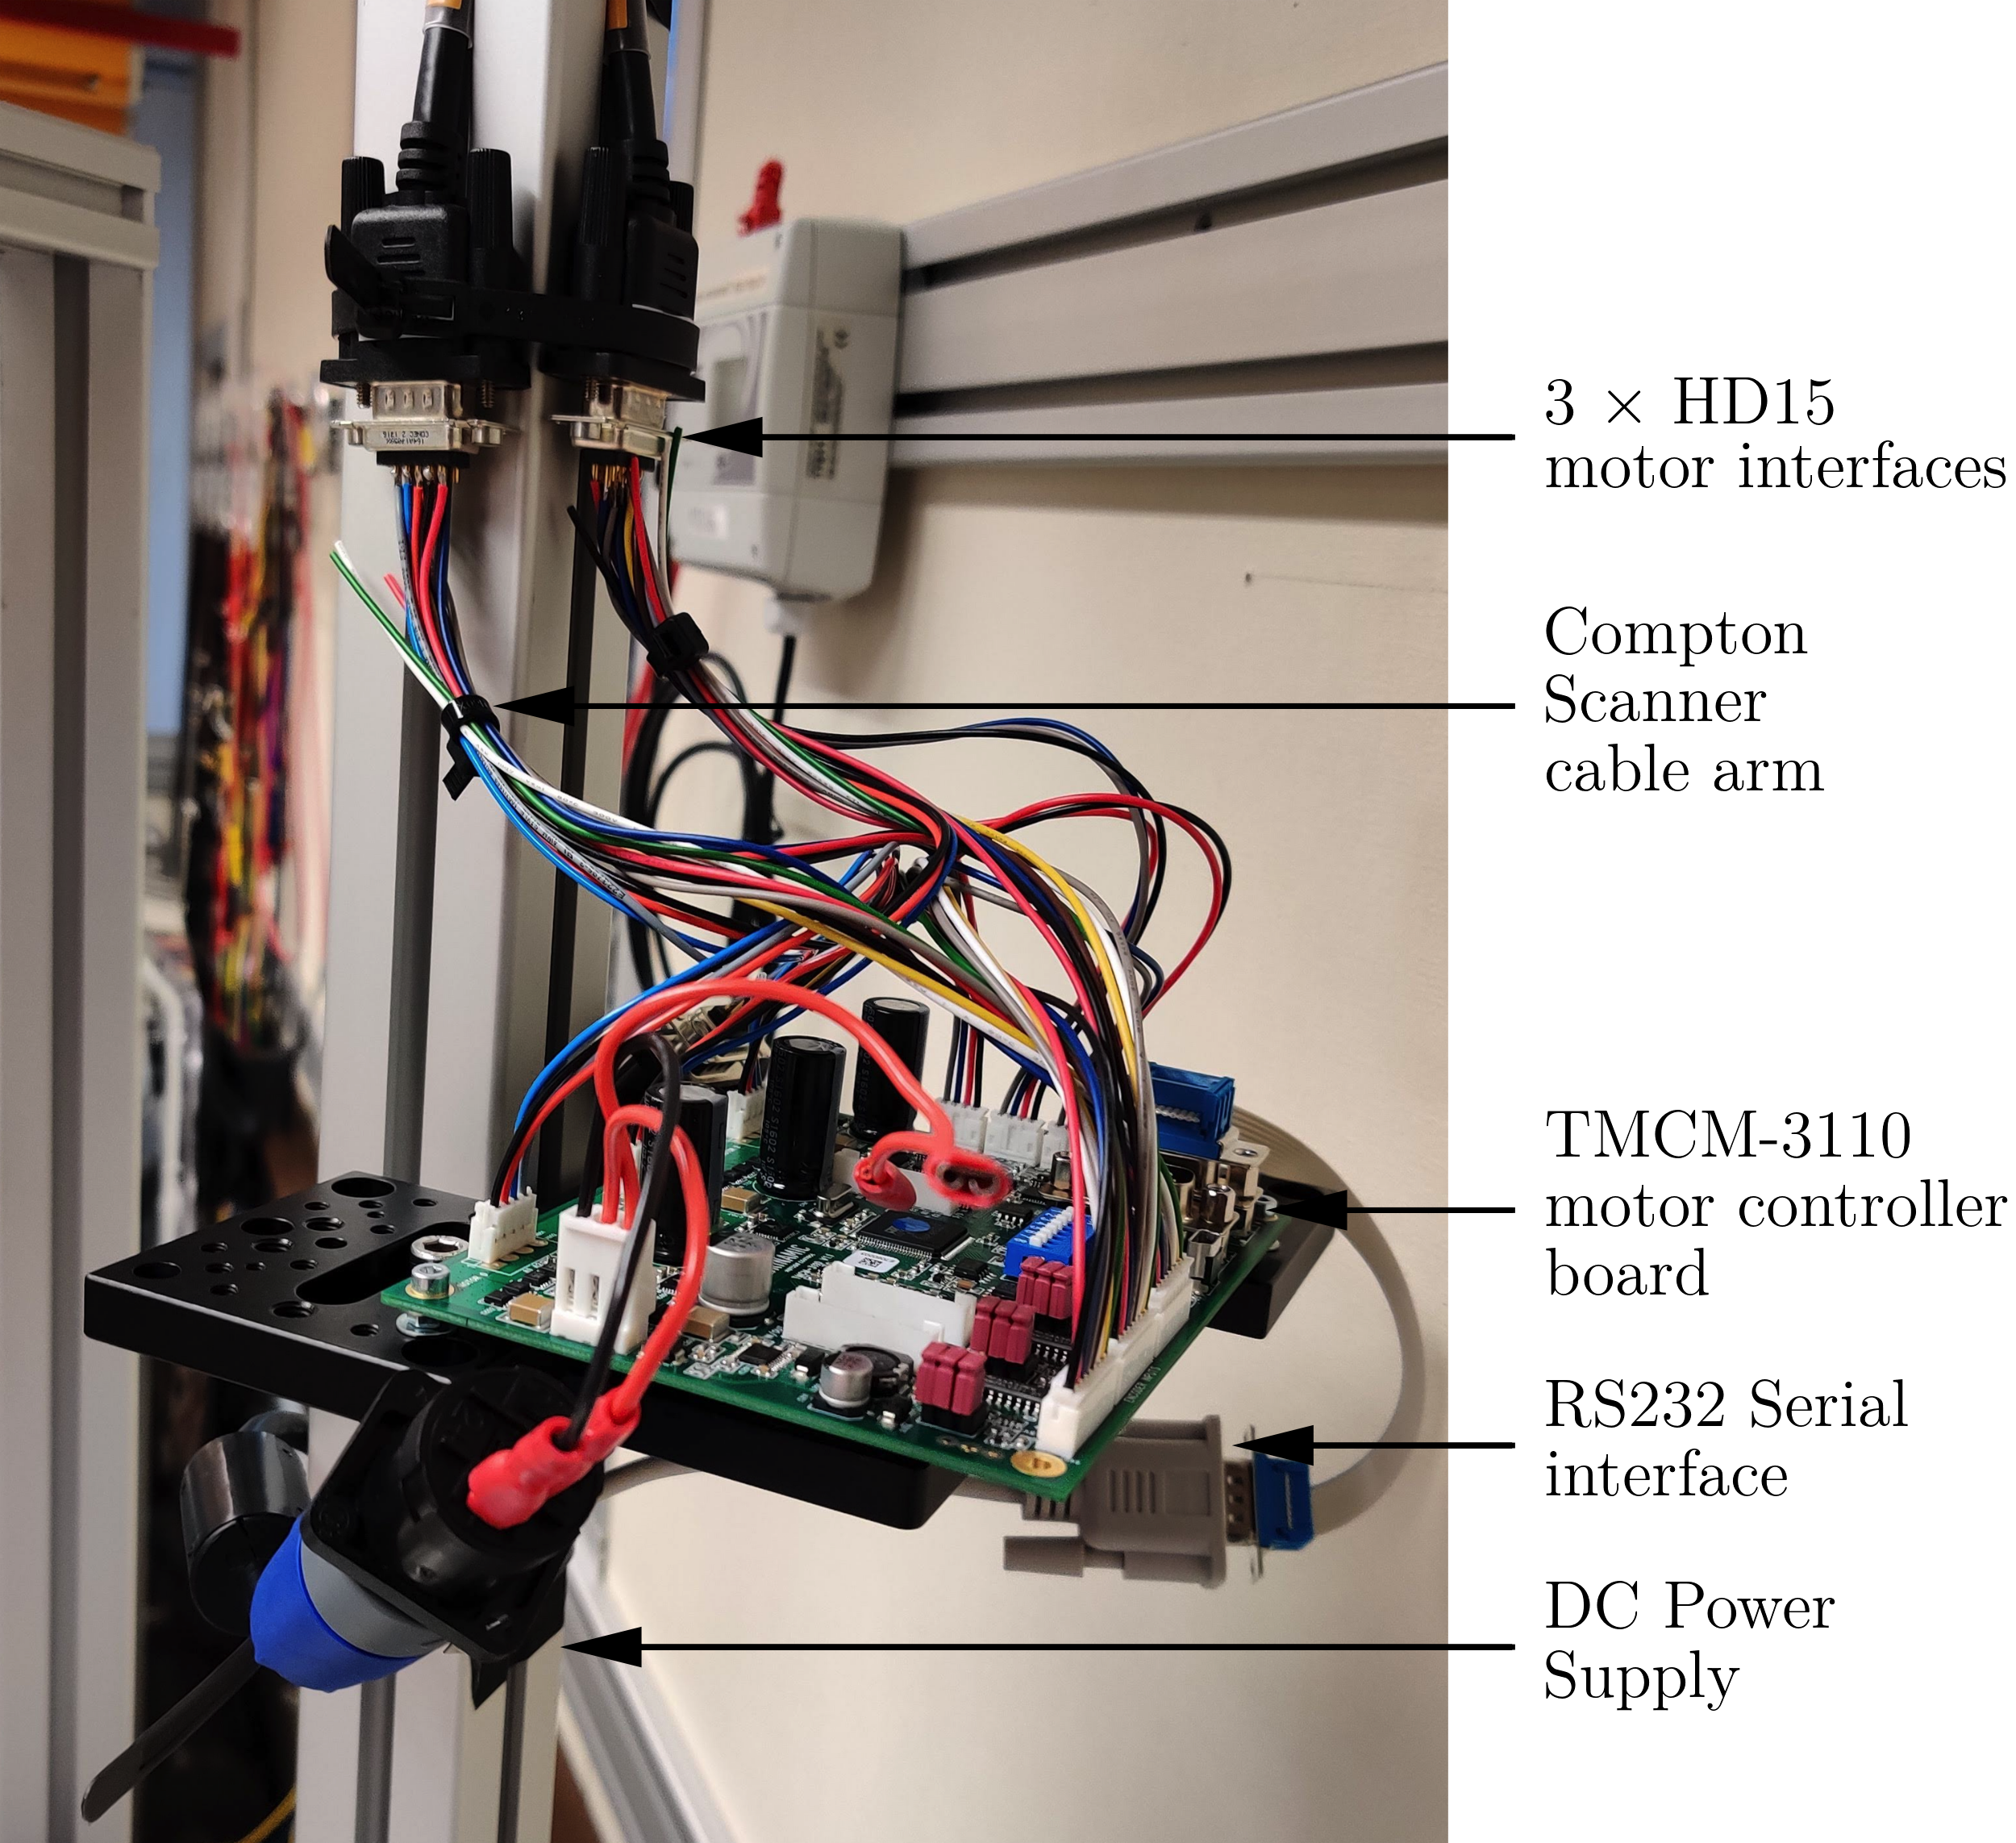
\includegraphics[width=5in]{figs/scanner/motor_control_labeled_width_5in.png}
	\caption{The fully operational motor control system prior to enclosure installation.}
	\label{fig:motorcontroller}
\end{figure}
The motor control system was built and programmed to interface with the two translational and one rotational motor stages (each controlled by a separate channel on the TMCM-3110 board). Thus, the system is fully customizable, allowing the user to set such motor parameters as acceleration, speed, and switch operation, on a channel by channel basis. These parameters were chosen with the load on each motor in mind to carefully and smoothly drive each motor stage. 
%A correctly programmed hardware switch will switch off a motor if it reaches the end of its track. However, this does not stop the motor if it encounters other objects in its path. This poses a problem for the vertical and horizontal motor stages, whose tracks could cause a collision between the source and camera. To remedy this a software switch was introduced which impedes the user from moving the camera into the path of the source. 

The user interfaces with the motor control system with a \julia{} software package. The package was designed to send encoded commands to the TMCM-3110's serial interface via a NetCom Plus 811 serial server. With this software the user can type simple command line instructions - such as move, calibrate, stop - via any terminal running \julia{} allowing for remote control of all motors via ssh. A network camera mounted on the crossarm aids in the safe remote operation of the motor system. 

\section{Commissioning Data}

An n-type segmented point-contact germanium detector with an energy resolution of 2.63\,keV at 356\,keV was used to take Compton scanner commissioning data. Monte Carlo simulations indicate that this energy resolution, and the geometry of the system, result in ``a FWHM resolution of less than $\pm1\,\text{mm}$ along the beam direction''~\cite{compton_scanner}. This detector was chosen because of the wealth of information the segmentation provides. Each event results in four pulses, corresponding to the point-contact and the three-fold segmentation contact readout. Thus, a single reconstructed event provides four pulses which can be compared to simulation. A pulse shape library was created for this detector along the $\langle100\rangle$ crystallographic axis and compared to \SSD{} simulations. The trends observed in data and simulation agree, which cross validated the position reconstruction described in this chapter and the fidelity of \SSD{} simulations for this detector. The commissioning data demonstrated that the goals of the Compton scanner -- most succinctly the $\pm1\,\text{mm}$ FWHM position reconstruction resolution and the drastic reduction in scanning times -- were met, paving the way for the application of the system to the next generation of Ge detectors. 

\chapter{Integration of an ICPC Detector}\label{chap:integration}

The n-type segmented point-contact germanium detector served as an effective test bench for the Compton Scanner. Building on this success, the Compton Scanner was integrated with a LEGEND ORTEC\textsuperscript{\tiny\textregistered} inverted coaxial point contact detector -- \IC{}. 

The detector was mounted in an ORTEC\textsuperscript{\tiny\textregistered} PopTop\textsuperscript{\tiny TM} cryostat with an attached cooling rod. This integrated system housed the detector in vacuum, along with an easily-accessible charge sensitive preamplifier and high-voltage (HV) filter. A single cable bundle exited the PopTop via a feedthrough which included coaxial cables for signal readout and pulser input, a SHV connector for HV input and a DB-9 connector for the low-voltage (LV) input to the preamplifier. The signal cable is connected to an analog-to-digital converter (ADC) (Section~\ref{sec:ic_det_intru}). To reach the cryogenic temperatures necessary for detector operation, the attached cooling rod was immersed in a 30L liquid nitrogen (LN$_2$) main dewar. In this system LN$_2$ boiled off at a rate of approximately 5\,L/day. Thus, a 150\,L LN$_2$ dewar was attached to refill the main dewar every three days. Four PT-100 thermoresistors~\cite{pt100} were placed along the length of the cooling rod and were connected to a temperature monitor (LAKE SHORE\textsuperscript{\tiny\textregistered} Model 218~\cite{lakeshore}) which was readout by the NetCom serial server of the motor control system. These data were used to determine the LN$_2$ level of the main dewar.  Each of these systems, ADC, LN$_2$ dewars, temperature monitor, and HV and LV supplies were placed in the periphery of the detector as shown in Fig.~\ref{fig:full_setup}. A table was built around the main dewar, with a hole cut out for the cryostat. The rotational motor and Compton Scanner frame were mounted on this table and the centers of the frame and the detector were aligned (See Section~\ref{sec:centeralignment}).

A PC was connected to the ADC with fiber optics to eliminate any noise-coupling into the system. The PC ran all data acquisition (DAQ) scripts and stored data locally on a 1.3\,TB solid state drive. Monitoring scripts on the DAQ PC collected and stored HV, temperature sensor, hard drive and Compton Scanner motor position data at 60\,s intervals. A compilation of the relevant data was live-streamed and available online from any web browser (Section~\ref{sec:monitoring}). All systems, except the ADC and the Compton Scanner camera system (due to noise coupling, Section~\ref{sec:noise}) were powered by a XANTO 3000R universal power supply (UPS)~\cite{ups} and had common ground. The cameras were connected to the same Ethernet switch as the DAQ PC and NetCom serial server and one sync line from each camera was connected to the ADC.

\begin{figure}[htb]
    \centering
    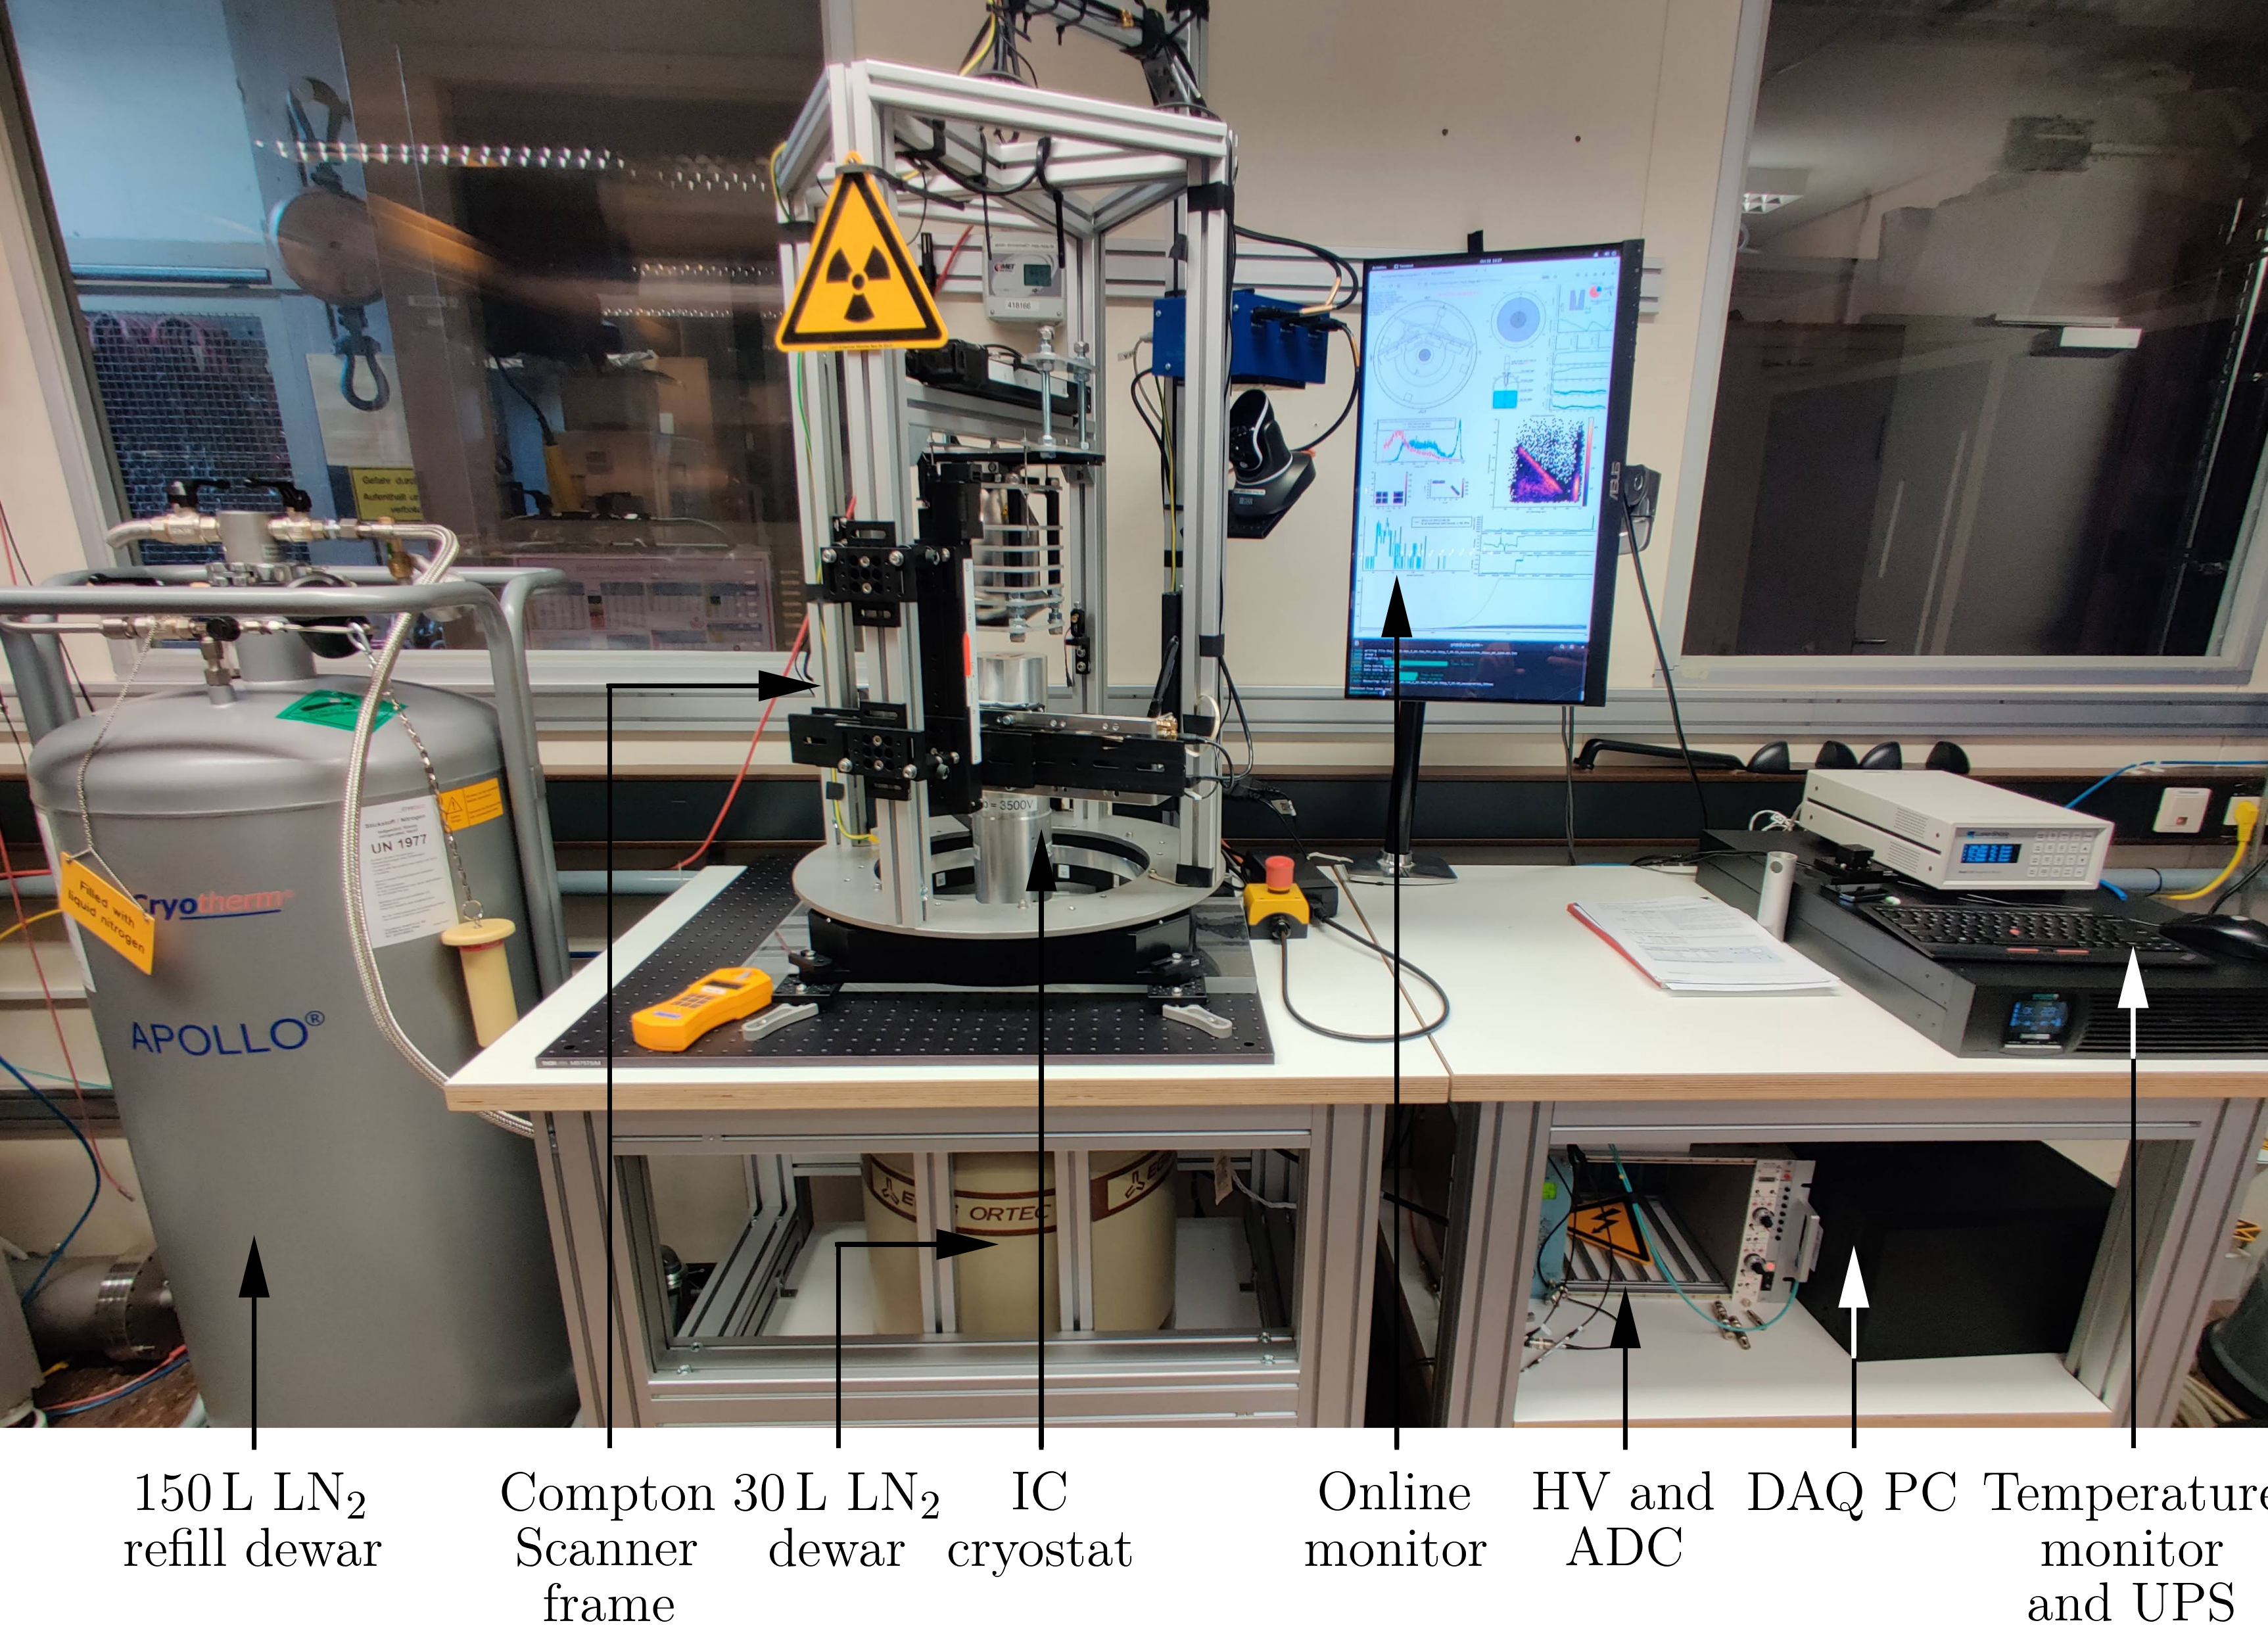
\includegraphics[width=6in]{figs/integration/full_setup_labeled_width_6_9.pdf}
    \caption{Integrated ICPC detector system with Compton Scanner frame.}
    \label{fig:full_setup}
\end{figure}

\section{ICPC Detector and its Instrumentation} \label{sec:ic_det_intru}

The geometry of the detector crystal and its contacts are shown in Fig.~\ref*{fig:ic_semiconductor} in the same orientation as in the cryostat (borehole facing dewar). The impurity concentration profile along the $\langle001\rangle$ crystallographic axis ($z$-axis in Fig.~\ref*{fig:ic_semiconductor}) was provided by the manufacturer. ORTEC used a Hall sensor to measure the impurity concentration of test slices that were cut from the regions adjacent to the top and bottom of the detector during manufacturing. The reported values at the top and bottom of the detector are $\rho_{\text{top}} = 1.109\times 10^{10}\,\text{cm}^{-3}$ and $\rho_{\text{bottom}} = 1.98\times 10^{10}\,\text{cm}^{-3}$ respectively. ORTEC recommended an operating bias voltage of 3500\,V, 550\,V over the measured depletion voltage.  
\begin{figure}[htb]
    \centering
    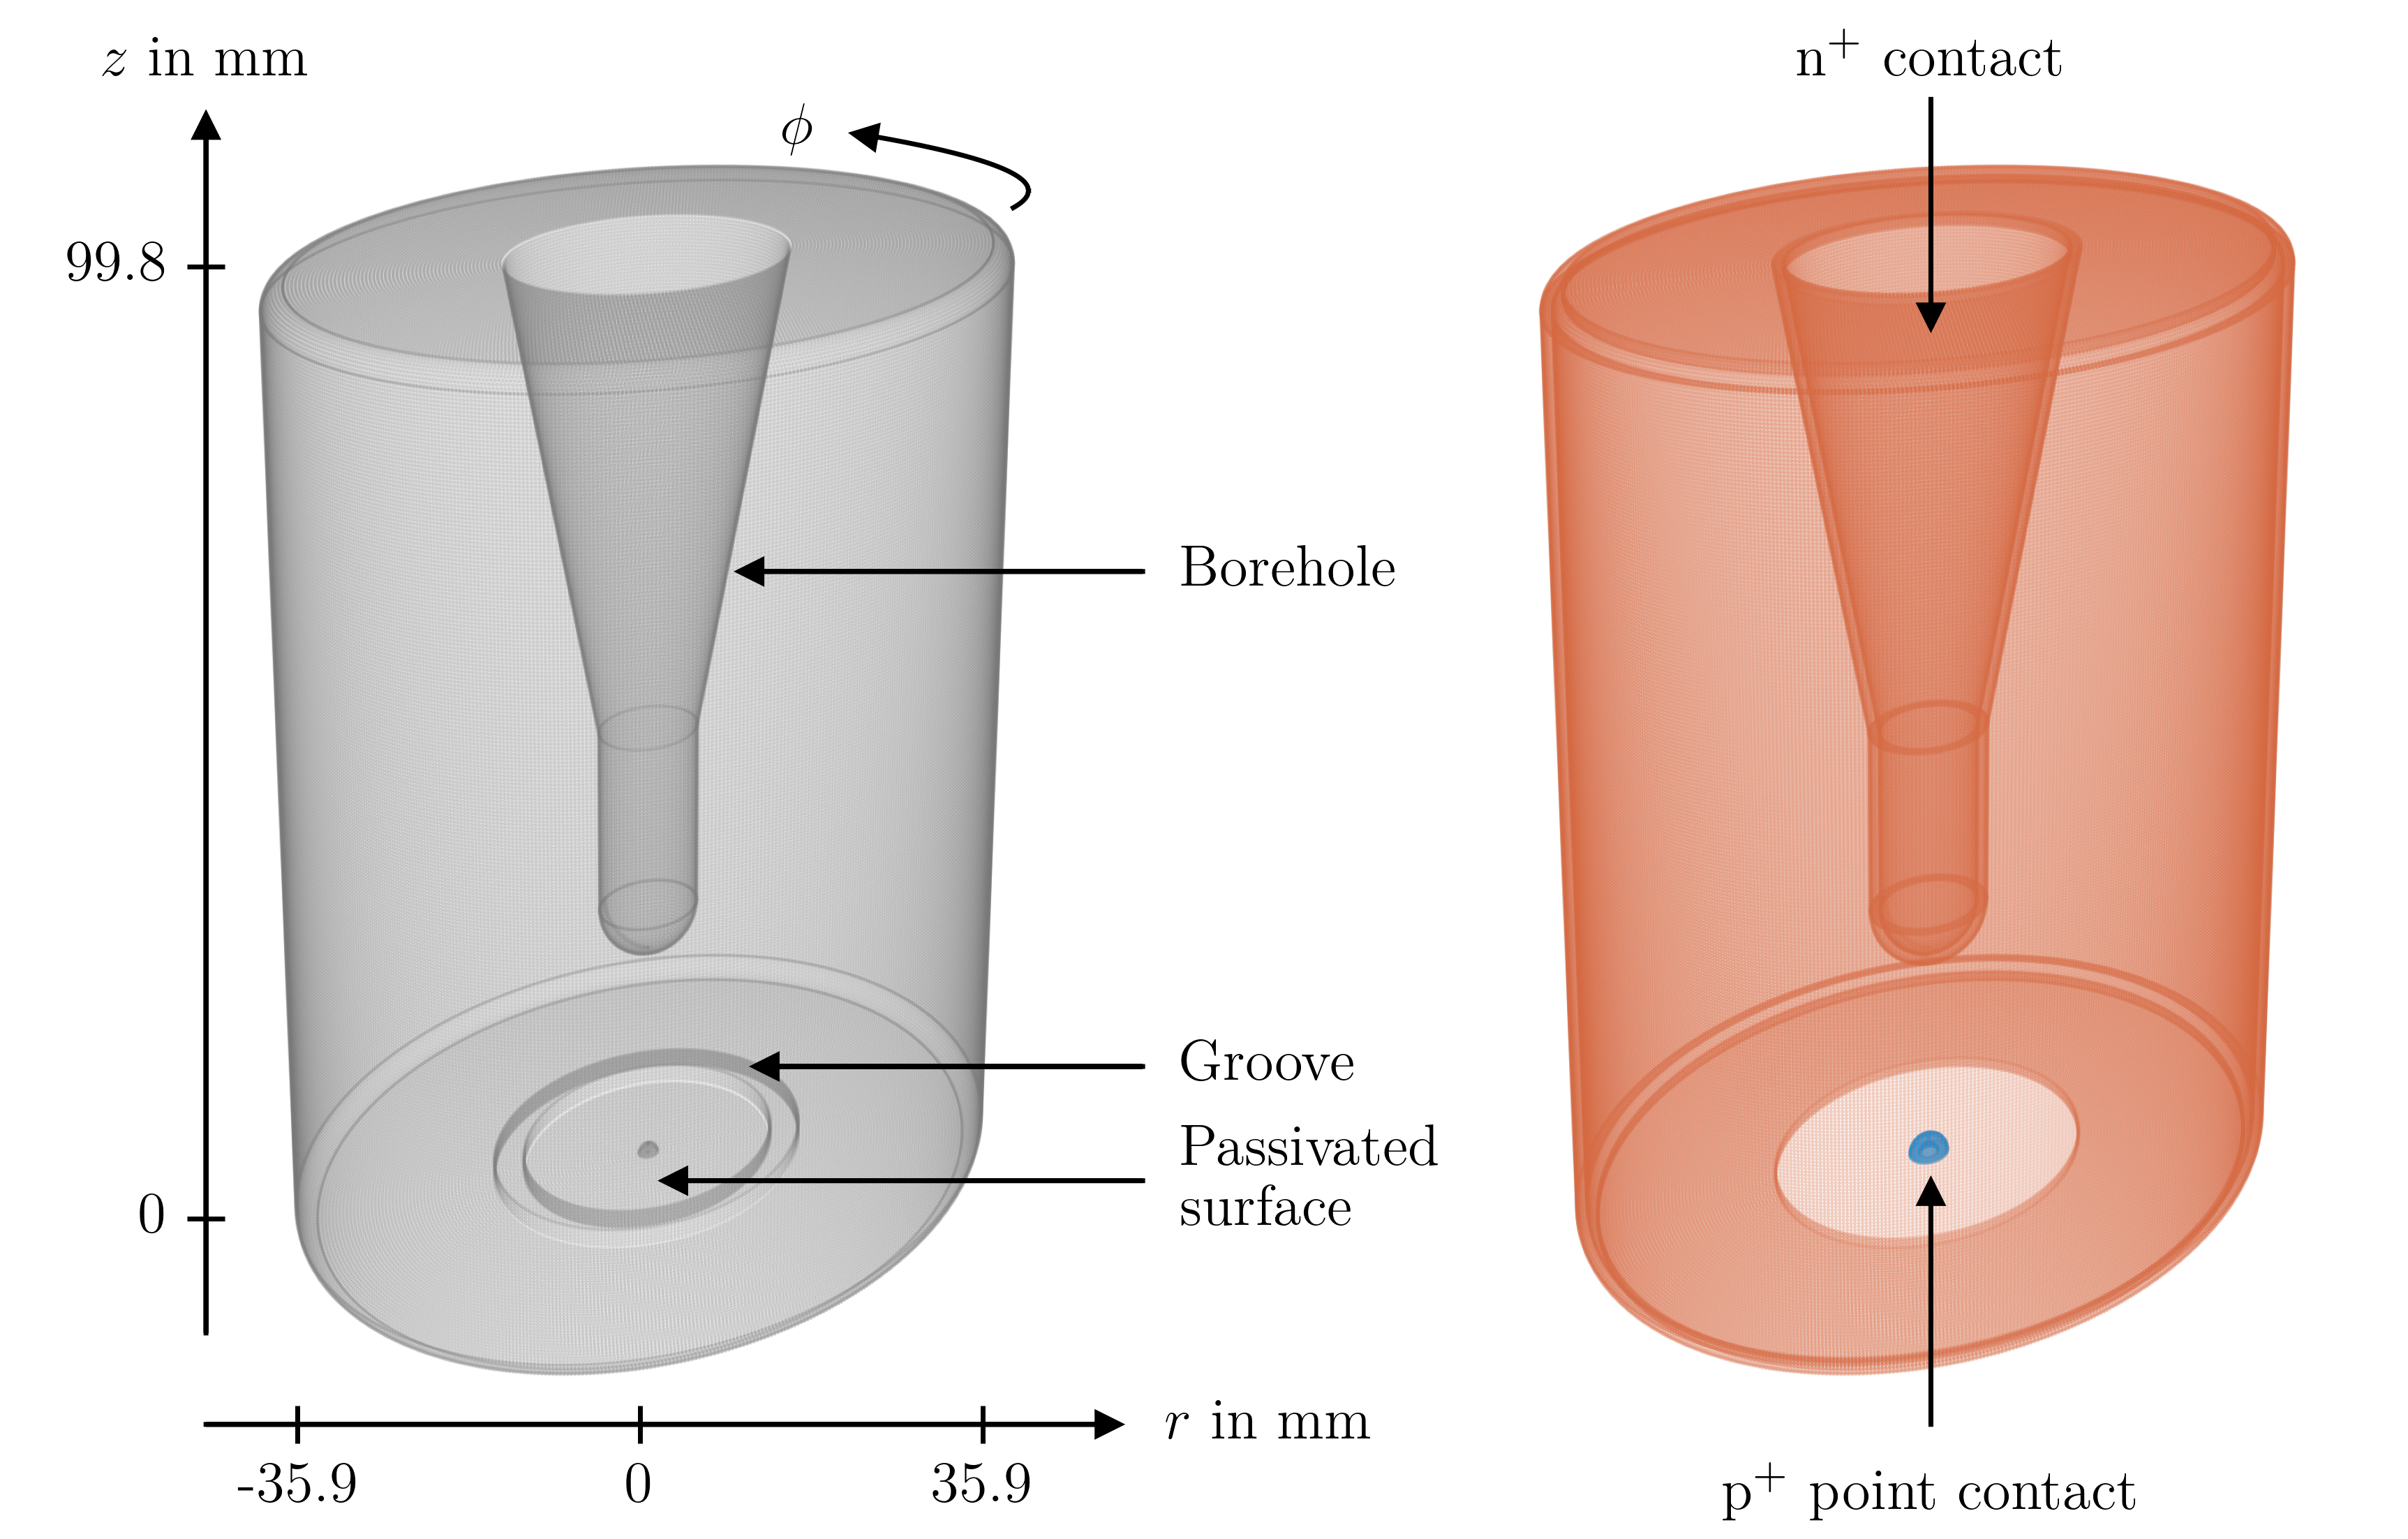
\includegraphics[width=6in]{figs/integration/P43511A_labeled_width_6_9in.pdf}
    \caption{Geometry of P43511A. The geometry of the crystal is shown in gray. The large n$^+$ contact and hemispherical p$^+$ contact on the surface of the crystal are shown in orange and blue respectively. The surface in between these contacts is passivated. Rendered with \SSD}
    \label{fig:ic_semiconductor}
\end{figure}

Upon receiving the detector at the Max Planck Institute for Physics, the four PT-100 thermoresistors were installed on the cooling rod and their cables were guided out of the dewar through the LN$_2$ vent tube shown in Fig.~\ref{fig:poptop}, before the first immersion into LN$_2$. The temperature of the detector was read out from a PopTop feedthrough connected to a MINCO-500 thermoresistor at the junction between the cooling rod and detector (see ``Temperature sensor'' in Fig.~\ref{fig:poptop_cicuit}). It was determined to be at a constant $(95 \pm 1)$\,K within a three-day LN$_2$ refill cycle and was checked periodically while data were not being taken - no deviations from this range were found.
\begin{figure}[htb]
    \centering
    \includegraphics[width=6in]{figs/integration/poptop_labeled.png}
    \caption{PopTop cryostat with attached cooling rod and dewar in horizontal configuration. Note that this system was used in the Compton Scanner frame in vertical configuration, i.e. the cooling rod is linear and not L-shaped as shown in this diagram, and thus the detector is centered and stacked on top the collar of the dewar~\cite{poptopmanual}.}
    \label{fig:poptop}
\end{figure}

\begin{figure}[htb]
    \centering
    \includegraphics[width=6in]{figs/integration/poptop_circuit_width_6_9in.pdf}
    \caption{PopTop cryostat circuit level diagram. Re-rendered from the GAMMA-X\textsuperscript{\tiny\textregistered} HPGe (High-Purity Germanium) Coaxial Photon Detector System manual~\cite{poptopmanual}}
    \label{fig:poptop_cicuit}
\end{figure}


The charges induced on the point-contact of the ICPC were amplified with an ORTEC charge sensitive preamplifier as shown at the circuit level in Fig.~\ref{fig:poptop_cicuit} and its placement relative to the detector in Fig.~\ref{fig:poptop}. The preamplifier was powered by an ORTEC NIM LV supply. The circuit was placed in ``Normal mode'' (as opposed to ``Differential mode'') and thus only the signal from Output 1 is readout.  The Output 1 signals were recorded using a 14-bit ADC (STRUCK SIS3316-250-14~\cite{STRUCK}), with a sampling frequency of 250\,MHz, resulting in 4\,ns samples.

HV was applied to the ICPC at the ``Bias'' input of Fig.~\ref{fig:poptop_cicuit} with a NHQ-226 dual-channel NIM HV supply~\cite{hvsupply}. The module is controlled remotely via its RS232 serial interface which is connected to the same NetCom serial server as the motor control system (Section~\ref{subsec:motorcontrol}) and LAKE SHORE temperature monitor. The \juliapackage{Sockets} module of the standard \julia{} library was used to communicate with the serial server. Once the bias voltage was set, fluctuations of up to 0.1\,V were observed. However, the HV supply automatically ramped down on many occasions (usually once per month, with frequency increasing towards the end of operation). HV discharges are suspected to be the cause of such automatic ramp downs.

%The automatic bias shutdown circuit was determined to be faulty and was not used. Therefore the HV cannot automatically ramp down if the detector looses cryogenic temperatures, thus a strict LN$_2$ refill schedule was observed and the LN$_2$ level in the main dewar was monitored constantly. 

%The serial commands and code-snippets necessary to control and read out the HV supply (and read out temperatures from the tempreature monitor) were previously written by Lukas Hauertmann and were incorporated into the Compton Scanner control and monitoring code.


\section{Data Acquisition}\label{sec:daq}

The data acquisition settings are set in a \textit{config.scala} file which is loaded into the STRUCK ADC. This file sets parameters such as channel readout, thresholds, online energy calculation, and the length of recorded traces. These parameters were chosen depending on the measurement performed. All measurements fall into one of four DAQ modes: Germanium, Compton, Hybrid, and Noise Characterization. 
\begin{table}[tbph]
    \centering
    \caption{DAQ Modes and their settings}\label{tab:daqmodes}
	\vspace{12pt}
    \begin{tabularx}{1\textwidth}{>{\tr}X >{\tr}X >{\tr}X >{\tr}X >{\tr}X}
		\hline \noalign{\vskip 1ex}
        DAQ Mode & Trace samples ($N_s$) & Threshold & Camera status & Coincidence filtering\\[1ex]
		\hline \noalign{\vskip 1ex}
		Compton & 5000 & 100 keV & ON & Active \\
		Hybrid & 5000 &  30 keV & ON & Inactive\\
        Noise & 65532 & 0 keV & ON/OFF & Inactive\\
		\multicolumn{5}{l}{Germanium} \\[1ex]
        \quad \BaS & 5000 &  30 keV & OFF & Inactive\\
		\quad \ThS & 5000 & 100 keV & OFF & Inactive\\
		\quad \CsS & 5000 & 100 keV & OFF & Inactive\\[1ex]
		\hline
    \end{tabularx}
\end{table}

In Germanium mode, only the ICPC data is of interest and therefore the Compton Scanner was not used. \BaS{} and \ThS{} data were taken with the \CsS{} source placed as far way from the detector as its track would permit, allowing for approximately 80\,mm between the collimator borehole and the edge of the detector in the $xy$-plane. The camera system was powered off in this configuration and only Output 1 from the detector was physically connected to the ADC to minimize noise. The threshold was set depending on the type of source used, in particular it was lowered to capture the 81\,keV line of \BaS{}. Note that the detector was only scanned with the \BaS{} source illuminating from the side. In this region the 0.5-1.0\,mm thick dead layer of the n$^+$ contact stops gammas from the 31\,keV line, which have an attenuation length of approximately 0.15\,mm~\cite{NIST}. 

In Compton mode, all Compton Scanner systems were operational and only events coincident in the detector and the camera system were targeted. The only source used in this mode was \CsS{}. As Section~\ref{subsec:camera} describes, the camera readout software is proprietary. Camera data is streamed over Ethernet to the DAQ PC and thus this system is fully independent of the germanium-ADC readout. Germanium and camera data are taken in parallel. To synchronize these data streams a sync line from each camera was connected to the ADC and sync pulses were sent every 2\,s. The resulting ADC trigger times were then used to time-align the data streams. Note that sync-pulse traces were also recorded. A 3.6\,kHz event rate was observed when the \CsS{} source was driven over the detector - except over the detector borehole where the rate decreases as expected. The corresponding data rate of 2\,GB/min, made it prohibitive to keep all the recorded data; therefore a filtering script, which ran in parallel to the germanium and camera DAQ systems, used the sync pulses to select camera and germanium events which fell within a 50\,$\upmu$s coincidence window: 
\begin{equation}
	\left|t_{_{\text{IC}}} - t_{_{\text{CAM}}}\right| < 50\,\upmu s
	\label{eq:coincidence_window}
\end{equation}

Where $t_{_{\text{IC}}}$ and $t_{_{\text{CAM}}}$ are the time-aligned event time stamps of the ICPC and the camera respectively. All other data were discarded, resulting in at least a factor of 10 data reduction. The 50\,$\upmu$s coincidence window is conservative - regardless of the synchronization technique used. Most coincident event candidates fell withing a 10\,$\upmu$s time window. 

Hybrid mode was used for alignment measurements, where all events in the camera and detector, not just coincident events, were of interest. These measurements are discussed at length in Section~\ref{sec:centeralignment} and Section~\ref{sec:detcamalignment}.

In Noise Characterization mode, only the noise in the ICPC traces is of interest. Therefore, the \CsS{} source is placed in the same location as in \BaS{}/\ThS{} Germanium mode and the threshold is reduced to a minimum to only trigger on noise. The trace length is set at the maximum to observe low frequency noise since it can degrade energy resolution. This mode is intended to characterize the noise in the ICPC traces while in Germanium and Compton hardware configurations as in Section~\ref*{sec:noise}.

The \julia{} package \juliapackage{StruckVMEDevices}~\cite{struckvme}, was used to interface with the STRUCK ADC. Therefore, as with motor, HV, and temperature monitor interfaces, data can be taken directly from the \julia{} terminal. When using this package in its original form, dead times of up to 45\% were observed. Therefore, a minor modification of the code was needed. After modification, the maximum dead time was 4\%.  

In all DAQ modes 2000 samples before each trigger are recorded, ensuring sufficient statistics for baseline removal and soft pileup flagging, offline event-onset determination and energy estimation.   

\section{ICPC Center Alignment and Drift}\label{sec:centeralignment}
To accurately reconstruct event positions in the ICPC, the Compton scanner's motor coordinates -- which set the position of the camera system and the \CsS{} source --  were converted into detector coordinates. This is most easily achieved when the ICPC and Compton scanner frame are concentric, thus aligning the horizontal motor track with the radial axis of the ICPC at all rotational motor angles, $\mathcal{A}$. In practice deviations between centers always existed, and given the small vibrations introduced by motor operation and LN fills, the centers drifted over time. The geometry resulting from the non-concentric operation condition is depicted in Fig.~\ref{fig:misalignment}.
\begin{figure}[htb]
    \centering
    \includegraphics[width=4in]{figs/integration/icpc_alignment_quantities_labeled_width_4in.png}
    \caption{The center misalignment parameters, as defined in the text, are shown. The shaded gray areas depict the ICPC, with the borehole in dark gray. The Compton scanner frame rotational position is depicted with a dashed circle.}
    \label{fig:misalignment}
\end{figure}

As shown in the figure, the horizontal motor track, with coordinate $\mathcal{H}$, deviates from the ICPC center by $\Delta \mathcal{H}$ (in the ICPC radial direction) at rotational motor position $\Delta \mathcal{A} - 90^\circ$. The detector edges are denoted by $\mathcal{H}_e$. To determine $\Delta \mathcal{H}$ and $\Delta \mathcal{A}$, $\mathcal{H}_e$ was estimated at various angles during center alignment campaigns.

To perform the initial center alignment, and to subsequently monitor any drift from this alignment, the ICPC was scanned over a radial range -- centered at the estimated location of the detector edge -- every $\mathcal{A} = 10^{\circ} - 15^{\circ}$. The event rates at each $\mathcal{A}$ are fit to Eq.~\ref{eq:edge_fit} to compute the edge location:
\begin{equation}
    N(\mathcal{H}) = \dfrac{N_0}{2} \left[ 1 + \text{erf}\left(\dfrac{\sqrt{2} (\mathcal{H} - \mathcal{H}_e(\mathcal{A}))}{R_{eff}}\right) \right] + N_\text{B},
	\label{eq:edge_fit}
\end{equation}
where $N(\mathcal{H})$ is the event rate at each horizontal motor position, $\mathcal{H}$, and $N_0$, $N_\text{B}$, $\mathcal{H}_e$ and $R_\text{eff}$ are the floating fit parameters corresponding to the background-subtracted event rate when the \CsS{} beam is fully on the ICPC, the background event rate, the detector edge and the effective radius of the beam. This radius results from combining the effects the ICPC n$^+$ dead layer and the Gaussian profile of the \CsS{} beam. The edge fits result in $(\mathcal{A}, \mathcal{H}_e)$ pairs, which were then fit to Eq.~\ref{eq:misalignment_fit}: 
\begin{equation}
	\mathcal{H}_e(\mathcal{A}) = \mathcal{H}_0 - \Delta \mathcal{H} \cos(\mathcal{A} - \Delta\mathcal{A}) \pm \sqrt{R^2 - (\Delta \mathcal{H})^2 \sin^2(\mathcal{A} - \Delta\mathcal{A})}~,
	\label{eq:misalignment_fit}
\end{equation}
where $R$ is the active radius of the ICPC and $\mathcal{H}_0$ is the horizontal motor position of the center of the ICPC when $\mathcal{A} = \Delta \mathcal{A}$. Assuming a 1\,mm n$^+$ dead layer, $R = 34.9$\,mm. The form of the misalignment fit (Eq.~\ref{eq:misalignment_fit}) can be derived from the geometry in Fig.~\ref{fig:misalignment}. 
\begin{figure}[htb]
    \centering
    \includegraphics[width=6in]{figs/integration/center_alignment.pdf}
    \caption{The location of the edge of the ICPC ($\mathcal{H}_e$) is estimated as described in the text and exemplified for $\mathcal{A} = 0^{\circ}$ in the data panel on the left. The process is repeated for all $\mathcal{A}$'s to produce the plots on the right. The edge extracted from the fit at each $\mathcal{A}$ is shown for the 2022-03-21 and 2022-09-05 calibrations in the top and bottom respectively. In the far left, a pictogram depicts a radial slice of the ICPC and a top view. The top view shows the \CsS{} source positions for the 2022-9-05 alignment.}
    \label{fig:center_alignment}
\end{figure}

Before the beginning of the main data taking campaign, a near-concentric condition was achieved by iteratively moving the Compton scanner frame with respect to the ICPC and performing center alignment scans and fits. In this process, it was concluded that motor operation and LN refills did not significantly alter the alignment. The best possible alignment was achieved on 2022-03-21, from which point the integrated system was not re-aligned. On 2022-06-20 and 2022-09-05 center alignment scan were performed, where the latter was taken close to the end of ICPC operations. Fig.~\ref{fig:center_alignment} depicts the edge fitting procedure, as well as the misalignment fits for the initial and final scans. The misalignment quantities deduced from the fits are summarized in Tab.~\ref{tab:misalignment}.
\begin{table}[tbph]
    \centering
    \caption{Summary of misalignment quantities derived from the three center alignment scans.}
	\vspace{12pt}
	\begin{tabularx}{1\textwidth}{>{\tr}X >{\tr}X >{\tr}X >{\tr}X}
		\hline \noalign{\vskip 1ex}
		Date & $\mathcal{H}_0$ in mm & $\Delta \mathcal{H}$ in mm& $\Delta \mathcal{A}$ in $^\circ$\\
		\hline \noalign{\vskip 1ex}
		2022-03-21 & $82.20 \pm 0.01$ & $0.47 \pm 0.01$ & $16.2 \pm 1.7$\\
		2022-06-20 & $82.15 \pm 0.01$ & $0.45 \pm 0.01$ & $28.5 \pm 1.9$\\
		2022-09-05 & $82.07 \pm 0.01$ & $0.66 \pm 0.01$ & $39.7 \pm 1.2$\\[1ex]
		\hline
	\end{tabularx}
	\label{tab:misalignment}
\end{table}

Although less accurate, scans across the full detector also estimate an ICPC center location of approximately 82\,mm, supporting the 1\,mm-dead-layer assumption, and the misalignment fits. It is clear that near concentric conditions were maintained during the main data taking campaign. Thus, in this work, the following concentric coordinate approximation is used to transform motor to detector coordinates $(r,\phi,z)$:
\begin{equation}
    r = 82\,\text{mm} - \mathcal{H},\quad \phi = \mathcal{A}
\end{equation}
If needed, the exact coordinate transformation can be performed as follows, using the most relevant misalignment quantities from Tab.~\ref{tab:misalignment}:
\begin{align}
    r &= \sqrt{\vert\mathcal{H} - \mathcal{H}_0\vert^2 + (\Delta\mathcal{H})^2 - 2 \Delta\mathcal{H} \vert\mathcal{H} - \mathcal{H}_0\vert \cos(\mathcal{A}-\Delta\mathcal{A})}, \label{eq:realr} \\ 
    \phi &= \text{asin} \left(\dfrac{\vert\mathcal{H} - \mathcal{H}_0\vert\sin(\mathcal{A} - \Delta\mathcal{A})}{r} \right) + \Delta\mathcal{A}~, \label{eq:realphi}
\end{align}

All measurements were performed in the $\|\mathcal{A} - \Delta \mathcal{A}\| < 60^\circ$ and $\|\mathcal{A} - (\Delta \mathcal{A} + 180^\circ)\| < 60^\circ$ ranges, thus in most cases the concentric approximation results in an under 2$^\circ$ deviation from the value calculated by Eq.~\ref{eq:realphi}. Only in the inner 10\,mm and far from $\Delta \mathcal{A}$ or $\Delta \mathcal{A} + 180^\circ$ is the deviation considerably larger. However, such deviations mostly fall within the angles subtended by the \CsS{} beam spot in these locations. For the entire detector, the concentric approximation results in an under 0.7\,mm deviation from the radial value calculated by Eq.~\ref{eq:realr}.

\section{ICPC - Camera Alignment} \label{sec:detcamalignment}
The hit positions in the camera data stream are given in local coordinates. Whenever camera (B) was used, its local coordinates were first transformed to the coordinate system of camera (A) as exemplified by Fig.~\ref{fig:czt_relative2D}. To perform position reconstruction, the camera coordinates were then transformed to into global coordinates, with an origin located at the bottom of the detector as shown by Fig.~\ref{fig:workingprinciple} and Fig.~\ref{fig:czt_icpc_alignment_pictures}. Note that $(x,y)$-alignment of the ICPC and camera is vital to the $z$-reconstruction, as the distance between the \CsS{} beam position and camera hit location appears in Eq.~\ref{eq:ztheta}. 

The horizontal motor track allows the \CsS{} to be placed over the camera (A). The \CsS{} beam was captured by the camera and shown in Fig.~\ref{fig:czt_icpc_alignment}. In this manner, a reference between the camera system and horizontal motor track is constructed, allowing for the calculation of the $(x,y)$-offset between the ICPC and camera (A). The marginalized beam profile (1-hit, 662\,keV events) is fit to a Gaussian in the $x$- and $y$-directions to calculate the center of the beam spot on the camera. 
\begin{figure}[htb]
    \centering
    \includegraphics[width=6in]{figs/integration/czt_icpc_alignment_pictures_labeled.png}
    \caption{The ICPC-camera alignment setup is pictured, where the \CsS{} source was moved to the right as to not block the view of the setup. The \BaS{} source swings to point at camera (A) and at the ICPC (middle and right pictures respectively).}
    \label{fig:czt_icpc_alignment_pictures}
\end{figure}

A similar strategy is used for $z$-alignment. A collimated \BaS{} source was temporarily mounted on a vertical motor stage, 90$^\circ$ from camera (A). The source could swing to point at camera (A) and at the ICPC while ensuring that the beam remained perpendicular to the $z$-axis. This temporary setup is shown in Fig.~\ref{fig:czt_icpc_alignment_pictures}. 
\begin{figure}[htb]
    \centering
    \includegraphics[width=6in]{figs/integration/czt_icpc_alignment_labeled_rq.png}
    \caption{\CsS{} and \BaS{} camera hits are shown in blue and orange respectively for the ICPC-camera alignment measurements in an isometric, top and lateral view of the integrated system. The later two views also feature the global coordinate system used. The sources were pointed in turn at camera (A), but the resulting hits are shown together for convenience. Camera (A) depicts \CsS{} 1-hit, 662\,keV events and \BaS{} 1-hit, 81\,keV and 356\,keV events. On the other hand, camera (B) shows all events from the \CsS{} measurement, predominantly Compton scatters from camera (A) and the surrounding structures. All components are rendered to scale.}  
    \label{fig:czt_icpc_alignment}
\end{figure}

A reference $z$-value was obtained by pointing the \BaS{} source to camera (A) and fitting $z$-profile of the beam (1-hit, 81\,keV and 356\,keV events) to a Gaussian. The \BaS{} source was also pointed at the ICPC, where an edge scan and fit (using the same techniques described in the last section) were performed to locate the top edge of the ICPC. In this manner the $z$-offset between the ICPC was and camera was found. Note that the camera is also on a vertical motor stage, thus a difference in camera motor positions is added to the $z$-offset when the camera is moved vertically from the position in which the alignment was performed. The \BaS{} beam was captured by the camera and shown in Fig.~\ref{fig:czt_icpc_alignment}.

In principle, the $z$-alignment is not needed, which is one of the advantages of the Compton reconstruction technique: the reconstructed $z$-position is simply offset by the $z$-position of the origin of the system of coordinates. However, performing this alignment had a twofold benefit. First it allowed for the camera to be optimally placed (before reconstruction) to target specific regions in the detector. Second, once reconstruction was performed, it served as a cross-check: giving the rage of $z$-values in which the reconstructed events should lie. 


\section{Noise} \label{sec:noise}
Test data were taken with the integrated the ICPC-Compton Scanner system in Compton and Germanium DAQ modes. A systematic analysis of data quality revealed large noise bursts in the waveforms collected in both DAQ modes. Two such events are plotted in Fig.~\ref{fig:burst_waveforms}. 
\begin{figure}[htb]
    \centering
	\vspace*{-10pt}
    \includegraphics[width=6in]{figs/param/burst_waveforms_6_9in.pdf}
	\vspace*{-10mm}
    \caption{Two waveforms exhibiting noise bursts in Compton DAQ mode. A burst obscures the beginning of the rise of the waveform on the bottom.}
    \label{fig:burst_waveforms}
	\vspace*{-5pt}
\end{figure}

The presence of bursts is not expected to deteriorate the energy resolution significantly, since the energy estimator (see trapezoidal shaping times in Section~\ref{sec:energy}) averages over a window many times longer than the period of the oscillations within a burst. However, the parameters calculated from pulse shape, such as the onset of the rise, $t_{0}$, are significantly impacted by the presence of bursts on the rising edge. The long traces taken in Germanium Noise Characterization mode (cameras off) reveal that bursts come in packets lasting longer than the maximum 262\,$\upmu$s recording time of the ADC. A burst frequency of 30\,kHz within a packet is determined from events like the one traced in Fig. \ref{fig:long_trace}. Each burst consists of two sub-bursts with an oscillation frequency of 11\,MHz and a separation of about 2\,$\upmu$s between centers. The estimated average amplitude of each burst is 42\,ADC units. Such an amplitude corresponds to roughly a quarter of that reached by a \BaS{} 81\,keV gamma event. 
\begin{figure}[htb]
    \centering
	\vspace*{-10pt}
    \includegraphics[width=6in]{figs/param/long_trace_width_6_9in.pdf}
	\vspace*{-10mm}
    \caption{A baseline subtracted event taken in Germanium Noise Characterization mode.}
    \label{fig:long_trace}
	\vspace*{-5pt}
\end{figure} 

To optimize data quality it is evident that events with noise bursts on or close to the rising edge of a waveform should be removed. Given that the event triggers are independent of the onset of bursts, the number of bursts at the rising edge can be estimated from any window of the same duration. The natural choice is to use the baseline. The baseline width, $B_w(N_s)$, defined as the difference between the maximum and minimum ADC value of the first $N_s$ samples in a waveform, is used to estimate the prevalence of noise burst events. From simulation (Section~\ref{sec:ic_sims}), the maximum drift time in the ICPC is approximately 2.2\,$\upmu$s, therefore a conservative window of $N_s = 1000$ samples (4\,$\upmu$s) is set for the rising edge. The $B_w(1000)$ distributions of test data taken in Compton and Germanium DAQ modes are shown in Fig.~\ref{fig:baseline_width_pre_optical}. Note that events with pileup were removed from both data sets using a technique that will be described in Section~\ref{sec:pileup}. 
\begin{figure}[htb]
    \centering
	\vspace*{-10pt}
    \includegraphics[width=6in]{figs/param/baseline_width_pre_optical_6_9in.pdf}
	\vspace*{-10mm}
    \caption{Baseline width distribution of $2.5\times10^4$ events taken in Compton DAQ mode and Germanium DAQ mode. Compton mode noise bursts are evident in the second peak in brown, centered around $B_w(1000) = 84\,\text{ADC}$. Baseline width of Germanium mode noise characterization data is fit to the high-energy-tail version of the response function of Eq.~\ref{eq:energy_peak_fit}.}
    \label{fig:baseline_width_pre_optical}
	\vspace*{-5pt}
\end{figure}

The overwhelming presence of burst events in Compton mode creates a clear separation between burst events and burst-free events in the $B_w(1000)$ distribution. Germanium mode test data is used to estimate $B_w(1000)$ for a population of burst-free events.  The main peak is fit to the same response function used for energy peaks (Gaussian plus exponentially modified Gaussian tail -- Eq.~\ref{eq:energy_peak_fit}), but with modifications to switch from a low-end to a high-end tail. A cut is set at the value where 99\% of the area under the fitted peak is covered. Events with $B_w(1000) > B_{w_\text{crit}}  = 53$\,ADC are chosen as burst event candidates. The resulting burst contamination in a 1000 sample window is 49\% and 4.6\% in Compton mode and Germanium mode test data respectively. It is clear that the camera system was introducing unacceptable amounts of noise into ICPC data. Steps were thus taken to isolate the camera system from the ICPC in hopes of matching the Germanium mode performance.

\section{Optical Isolation}
Germanium mode performance was optimized using $B_w(1000)$ as a figure of merit, prior to camera-ICPC isolation. Lower modes of the $B_w(1000)$ distribution indicate lower overall noise amplitude, while significant high-value tailing or secondary peaks indicate noise bursts. With this in mind, data were taken in dozens of grounding and power configurations. This campaign led to the final configuration of the system, which minimized, but did not fully eliminate the presence of bursts and lowered the overall noise amplitude. An overview of this configuration follows
\begin{enumerate}
	\item The ADC was coupled to the DAQ PC directly with fiber optics. This eliminated a ground loop created by the ADC-Ethernet-Switch copper connections. Note that camera system needs to be connected to this Ethernet Switch. 
	\item All systems were powered from the same UPS except the ADC. When the camera system was put into operation, the best performance was achieved when it was powered from a different source than the ADC and the UPS. 
	\item All large metal components surrounding the ICPC cryostat were grounded to the same ground of the UPS. This includes the Compton Scanner frame, aluminum breadboard, and camera enclosures.  
\end{enumerate} 

Reintegration of the camera system was investigated with the new integrated hardware configuration. Once again, when cameras were turned on, the prevalence of bursts increased. However, a significant reduction of bursts was observed when the sync copper cables of both cameras were disconnected from the ADC, an effect that had not been observed previous to the grounding and cabling changes. Due to hardware limitations, sync pulses could not be sent over optical fibers, however optical isolation can still be achieved by placing a IL300 optocouple~\cite{il300} in each camera copper sync line as Fig.~\ref{fig:optocoupler} shows.   
\begin{figure}[htb]
    \centering
	\vspace*{-10pt}
    \includegraphics[width=5.5in]{figs/param/optocoupler_circuit_width_5_5in.pdf}
    \caption{The IL300 integrated circuit~\cite{il300} is placed in the sync line from each camera to the ADC to send sync pulses without a copper connection.}
    \label{fig:optocoupler}
	\vspace*{-5pt}
\end{figure}

Each camera outputs a $V_{\text{sync}} = 3.3$\,V sync pulse.  The sync pulse length was set to match the switching time of IL300: 1\,$\upmu$s. The duration of the pulse was originally set to 50\,ns, resulting in the copper sync pulse shown in Fig.~\ref{fig:sync_pulses}. The resistance on the camera sync line, $R_{\text{sync}} = 100\,\Omega$, was chosen to drive the infrared LED in IL300 ($V_\text{d} = 1.25$\,V) with a current of $I_{sync} = (V_{\text{sync}} - V_\text{d})/R_{\text{sync}} \approx 20$\,mA, to not draw too much current from the camera. This current is sufficient to drive the LED in its optimal range~\cite{il300}. The two photodiodes in IL300 are operated in photovoltaic mode and their output is recorded by the ADC. $V_{\text{out}} \approx 5$\,mV is estimated from the amplitude of resulting optical sync pulses such as that in Fig.~\ref{fig:sync_pulses}.
\begin{figure}[htb]
	\centering
	\vspace*{-10pt}
    \includegraphics[width=6in]{figs/param/sync_pulses_width_6_9in.pdf}
	\vspace*{-10mm}
	\caption{A 50\,ns, 3.3\,V sync pulse saturates the ADC with a direct copper connection. In the same frame, but with different $y$-scale, the optocoupler response to a 1\,$\upmu$s, 3.3 V sync pulse is shown.} 
	\label{fig:sync_pulses}
\end{figure}
The vastly different rise times of the copper and optical sync pulses can be seen from their scales in Fig.~\ref{fig:sync_pulses}.  Nevertheless, the coincidence window is 50 times wider than the 1\,$\upmu$s risetime of an optical sync pulse. Thus, it is expected that the longer risetimes of the optical sync pulses does not significantly affect the number of events falling within the coincidence window. This becomes evident from the distribution of $t_{_{\text{IC}}} - t_{_{\text{CAM}}}$ within the coincidence window shown in Fig.~\ref{fig:coincidence_window}. A 5.5\% drop in coincidence rate is found with the introduction of the IL300 optocouplers in the sync lines. 
\begin{figure}[htb]
    \centering
	\vspace*{-10pt}
    \includegraphics[width=6in]{figs/param/coincidence_window_6_9in.pdf}
	\vspace*{-10mm}
    \caption{ Distributions of $t_{_{\text{IC}}} - t_{_{\text{CAM}}}$ in the 50\,$\upmu$s coincidence window for 3100\,s of Compton mode data taken with the IL300 optocoupler placed in the sync lines (Optical) and without (Copper). The coincident event rates are 147.3\,Hz and 155.8\,Hz respectively.}
    \label{fig:coincidence_window}
	\vspace*{-5pt}
\end{figure}

The optimized Germanium and Compton hardware configurations were tested in Noise Characterization DAQ mode. Compton data were taken with the IL300 optocoupler placed in the sync lines and without, which are referred to as the optical sync and copper sync configurations, respectively. The optical sync configuration matched the noise performance that was achieved by disconnecting the sync cables from the ADC. For the optical and sync configurations, data were taken with camera (A) on and camera (B) off, and with both cameras on. Germanium mode data were taken to establish the baseline noise performance.  

%A baseline selection criterion is established by calculating the root-mean-square (RMS) of the mean ADC values of background-free population of waveforms. These events are selected from 24000 Germanium mode data events. The mean of the first 200 samples is subtracted from each waveform. Events where the mean of the next 1000 samples is $\ge0$\,ADC are selected. This automatically eliminates soft pileup. Non-baseline events are dominated by background radiation. The probability of a background event falling within an event window ($\Delta t$), given a background rate of $r$, is calculated with the Poisson distribution.
%\begin{equation} \label{eq:poisson}
	%P(n = k) = \frac{(r\Delta t)^{k}e^{-r\Delta t}}{k!}
%\end{equation}
%The probability of zero background events ($k = 0$) falling within an event window of $\Delta t = 1000 \times 4\,\text{ns}$ is 99.9\%, given the 100\,keV-threshold background rate of 302\,Hz (calculated in Section~\ref{sec:centeralignment}). Even with a conservative $10 \times$ higher background -- to account for the 0\,keV threshold that was used here -- the probability only descends to 98.6\%. Thus, the selected events are overwhelmingly baseline events within the 1000-sample window. The RMS of the means of these 1000-sample windows is then calculated (RMS$_{\mu 1000}$) and and and upper limit is set at $5\text{RMS}_{\mu 1000}$. Each waveform is then averaged in 1000 sample intervals. If the mean any interval is above $5\text{RMS}_{\mu 1000}$ the waveform is tagged as a non-baseline. This technique eliminates most soft and hard pileup events and other background events or anomalous waveforms. 76.9\% of events survive the baseline cut.

%Background radiation will either be seen as a trigger within the $\Delta t_\text{event} = 65532 \times 4\,\text{ns}$ event window or as a decaying baseline if the trigger occurs before the event window (soft pileup). The average background energy (with 100\,keV threshold) is 315\,keV which corresponds to $\text{max(ADC)} \approx 566\,\text{ADC}$. The decay constant calculated in Section~\ref{sec:electronicsresponse}, $\tau = 55.53\,\upmu$s, is used to establish the decay window of $\Delta t_\text{decay} = n_\text{decay}\tau$. A baseline is counted as restored if the 1000-sample-mean ADC value of a waveform falls below the expected value of $5\text{RMS}_{\mu 1000}$. From $\text{max(ADC)}e^{-n_\text{decay}\tau} = 5\text{RMS}_{\mu 1000}$, $n_\text{decay} = 4.9$ is extracted. Setting the probability of finding no background events within the decay window and the subsequent event window ($\Delta t = \Delta t_\text{decay} + \Delta t_\text{event}$) in Eq. \ref{eq:poisson} to the baseline cut survival probability, the true background rate can be calculated. From this, a 494.8\,Hz 0\,keV-threshold background rate is determined. Note that this corresponds to a very reasonable 1.64 times higher background rate than that with a 100\,keV threshold.

The performance of the 5 hardware configurations is characterized by taking a Fast Fourier Transform (FFT) of each waveform and then averaging the FFTs in each data set. To ensure the fidelity of the averaged FFT, FFTs are only be performed on baselines. To remove background events, an offline trigger in the form of the trapezoidal filter (with parameters equal to that of the pileup trapezoidal filter -- Sec.~\ref{sec:pileup}) was used. Events which triggered were removed from the analysis and the FFTs and $B_w(1000)$ distributions are calculated for each data set. The $B_w(1000)$ distributions of all 5 hardware configurations are shown in Fig.~\ref{fig:baseline_width_optical}. As expected Germanium mode noise amplitude is the lowest overall and exhibits the lowest prevalence of bursts. There is a clear suppression of burst abundance in data taken with optical sync lines with respect to their copper sync line counterparts. In both cases, bursts are most prevalent when both cameras are operated. Nonetheless, near-germanium-mode performance was achieved in Compton mode with optical sync lines and camera (B) off. As in Section~\ref{sec:noise}, $B_w(1000)$ for a population of ``burst-free'' events is calculated from Germanium mode data.
\begin{figure}[htb]
    \centering
	\vspace*{-10pt}
    \includegraphics[width=6in]{figs/param/baseline_width_all_modes_6_9in.pdf}
	\vspace*{-10mm}
    \caption{Baseline width distribution of $1.5\times10^5$ events in all 5 hardware configurations.}
    \label{fig:baseline_width_optical}
	\vspace*{-5pt}
\end{figure}

Setting a 99.9\% fitted peak area coverage, events with $B_w(1000) > B_{w_\text{crit}}  = 49$\,ADC are chosen as burst event candidates. Note that a higher coverage of the main peak is used due to the clearer separation of burst and non-burst events in comparison to test data. Setting this cut, a lower sacrifice of non-burst events is obtained. Burst abundance is quantified from the distributions in Fig.~\ref{fig:baseline_width_optical} with the described cut value and presented in Tab.~\ref{tab:noise_results}.
\begin{table}[tbph]
	\centering
	\caption{Burst abundance in a 1000-sample window of test data and the five hardware configurations described in the text. The abundance is calculated as the fraction of events passing the $B_w(1000) \ge B^\prime_{w_\text{crit}}$ and $ B_w(1000) \ge B_{w_\text{crit}}$ cuts for test data and noise characterization data respectively.} 
		\vspace{12pt}
		\begin{tabularx}{1\textwidth}{bsss}
			\hline \noalign{\vskip 1ex}
			DAQ Mode & No sync & Copper sync & Optical sync\\[1ex]
			\hline \noalign{\vskip 1ex}
			Germanium test & 0.046 & -- & --\\
			Compton test (cam (A,B) on) & -- & 0.49 & --\\
			Noise -- Germanium & 0.026 & -- & --\\
			Noise -- Compton: Cam (A) on & -- & 0.095 & 0.027\\
			Noise -- Compton: Cam (A,B) on & -- & 0.24 & 0.15 \\[1ex]
			\hline
		\end{tabularx}
		\label{tab:noise_results}
\end{table}

A separate FFT was produced for burst-free Germanium mode data ($B_w(1000) \le B_{w_\text{crit}}$) and burst-dominant Germanium mode data ($B_w(1000) > B_{w_\text{crit}}$). To identify the signatures in the FFT for burst events. Busts can be identified by increased noise levels and large oscillations in the expected 9 - 20\,MHz range in Fig.~\ref{fig:fft_ge_log}. By comparing optical sync pulse data to copper sync pulse data in this range for both camera configurations (Fig.~\ref{fig:fft_ge}), there is a clear suppression of bursts in optical sync line data.
\begin{figure}[htb]
    \centering
	\vspace*{-10pt}
    \includegraphics[width=6in]{figs/param/fft_ge_mode_log_width_6_9in.pdf}
	\vspace*{-10mm}
    \caption{FFTs of 5\,min of burst-free and burst-dominated Germanium mode data. Note that all noise characterization measurements incur an 83.8\% deadtime.}
    \label{fig:fft_ge_log}
	\vspace*{-5pt}
\end{figure}

\begin{figure}[htb]
    \centering
    \includegraphics[width=6in]{figs/integration/ffts_5_modes.pdf}
    \caption{FFTs of the five hardware configurations described in the text in the 1-20 MHz
	range. From top to bottom: burst-free and burst-dominated Germanium mode data is compared. The combination of these populations (simply Germanium mode in the second and third panel) is compared with Compton data taken with only camera (A) on and then with camera (A) and (B) on. For Compton mode data, the copper and optical results are shown. Five minutes of data is used to construct each FFT.}
    \label{fig:fft_ge}
\end{figure}

Optical isolation of the sync lines was achieved with a minimal impact to coincidence rates while reducing the abundance of bursts within a 1000-sample-window by at least a factor of 2. Therefore, the integrated ICPC - Compton Scanner system adopted this technique to synchronize the camera and germanium data streams. Nevertheless, there is no free lunch. In principle, timing information from the cameras can be used to determine the onset of the rise, $t_0$, in germanium events. While the 1\,$\upmu$s risetime of sync pulses is negligible in a 50\,$\upmu$s coincidence window, it is not within the 4\,$\upmu$s risetime window of an ICPC event. Thus, a degradation of the $t_0$ resolution, as determined from trigger times in the camera system, is expected. The main culprit of noise bursts can now be identified as camera (B). Even with the optical sync lines, the burst abundance in 1000-sample window of 15\% was considered too high and camera (B) was powered off for most of the data taking campaign. 

\section{Monitoring} \label{sec:monitoring}
\begin{figure}[H]
    \centering
    \includegraphics[width=5.4in]{figs/integration/icpc_monitor.png}
    \caption{Online monitor depicting the real-time data described in the text.}
    \label{fig:remote_monitoring}
\end{figure}

The Compton scanner and ICPC data were monitored via a web interface. The web interface consisted of multiple images which depicted real time operational and data quality parameters including motor position, LN$_2$ levels, HV status, hard drive usage, waveform baselines, burst abundance, and offline coincidence filtering status. A capture of the web interface is shown in Fig.~\ref{fig:remote_monitoring}.

\chapter{Waveform Parameters}\label{chap:param}

To reconstruct event position, ICPC, camera, and ICPC-camera alignment parameters are needed. So far, two of these pieces have been presented: the camera parameters (position and energy) are directly given by the camera's proprietary software, and the ICPC-camera alignment parameters were calculated in the previous chapter. Nevertheless, one key piece of the puzzle is missing: ICPC energy.

This chapter is concerned with the information that can be extracted from ICPC waveforms, in particular, energy. Energy estimation itself depends on other waveform parameters, which are also presented. In the energy estimation process, waveforms are corrected for electronics response, a step also necessary to create a pulse shape library for the detector. The high activity of the \CsS{} source and large volume of the ICPC lead to a high pileup rate. Instead of discarding all of these events, corrections are applied when possible, in many cases doubling the amount of usable data. This chapter describes pileup classification and corrections, which result in two data streams subsequently used for ICPC position reconstruction.

An analysis toolkit -- based on the ultra-fast and GPU compatible waveform transformation functionality of \juliapackage{RadiationDetectorDSP}~\cite{rddsp} -- was built to calculate the waveform parameters. The code was purposely kept general, with the intent of future integration with the \julia{} software stack of the LEGEND experiment.

\section{The Reader's Guide to Pictograms}

Throughout this chapter and the ones that follow, data that were collected with various types of sources are presented, often alternating between measurements. Tab.~\ref{tab:daqmodes} summarizes the sources and DAQ setting used for each. Furthermore, the sources illuminated the ICPC in different directions and positions, leading to an increasingly large number of possible geometric configurations. Instead of just stating the source and geometric configuration in text, figures are aided by the inclusion of a pictogram on the left of each plot. These pictograms are intended to be self-explanatory cartoons of how the data shown in each figure were obtained. If the exact source positions are relevant, they are explicitly stated in the text. The five pictograms employed are shown in Fig.~\ref{fig:pictograms}. 
\begin{figure}[htb]
    \centering
    \includegraphics[width=6in]{figs/param/pictograms.pdf}
    \caption{Five pictograms representing data taken with the ICPC and \CsS{}, \BaS{} and \ThS{} sources.}
    \label{fig:pictograms}
\end{figure}

\noindent Going from left to right, the pictograms depict the following ICPC-source configurations. Note that where relevant cylindrical coordinates are given.
\begin{enumerate}
	\item Collimated \CsS{} source irradiating from the top at $(r_0,\phi_0)$ shown by the red line in the $\phi=\phi_0$ radial slice and red dot in the top view.
	\item Same as Pictogram 1, but only coincident events between the ICPC and camera are recorded. The camera and ICPC are shown to scale as is their relative $z$-position. However, the radial distance between the inner edge of the camera and the outer edge of the ICPC of 24.8\,mm is not shown to scale. 
	\item Collimated \BaS{} source irradiating from the side at position $(\phi_0,z_0)$ shown in the $\phi=\phi_0$ radial slice and top view. The much shorter range of \BaS{} gammas is illustrated with a short red line.
	\item Flood \ThS{} source placed concentric with the top of the ICPC, 14\,cm away. The distance between the top of the ICPC and the source is not shown to scale. 
	\item Flood \ThS{} source placed level with the p$^+$ contact and 9\,cm away from the outer edge of the ICPC. The distance between outer edge of the ICPC and source is not shown to scale. 
\end{enumerate}
The following is common to pictograms 1-3: The fast and slow axes of the ICPC are represented by dotted and dashed lines in the top view respectively. The following is common to pictograms 1-2: If data for more than 2 source positions is included in a figure, only the top view will show the source positions. If no source (red dots or lines) is shown on the pictogram, then it represents a background measurement. 

\section{Electronics Response}\label{sec:electronicsresponse}

The effects of the circuit shown in Fig.~\ref{fig:poptop_cicuit} are most succinctly observed in raw waveforms -- the output signals from the ADC -- as a baseline offset and exponentially decaying tail. These effects can be seen in Fig.~\ref{fig:baseline_removal} and Fig.~\ref{fig:decay_correction} respectively. The charge sensitive loop outputs an exponentially decaying signal with characteristic decay constant, $\tau_f = R_fC_f = 2$\,ms. The decay constant seen in data is the result of convolving this signal with the differentiator in the secondary amplification stage, which had a much sorter decay constant. 
%check tau with ORTEC

Prior to any waveform analysis, the baseline and tail decay were corrected. By fitting the first 1000 samples of a waveform to a line, the baseline offset ($B_o$) was calculated. In the low-event-rate regime, this value corresponds to a stable DC-offset (a resting baseline) on top of which signals evolve. However, higher rates drastically increase the probability that successive events occur before resting baseline conditions are restored. Although the decay is mostly governed by the second stage time constant, the convolution with the output of the charge sensitive loop introduces an undershoot from the DC-offset which recovers in the relatively long timescale characterized by $\tau_f$. Thus, as seen in Fig.~\ref{fig:baseline_removal}, the baseline offset distribution is highly asymmetric, with the events falling under the mode of the distribution resulting from this undershoot. The mode of the distribution provides a good estimate of the DC-offset. 
\begin{figure}[htb]
    \centering
    \includegraphics[width=6in]{figs/param/baseline_removal_6_9in.png}
    \caption{The first 1000 samples of 200 example raw waveforms (left) and baseline offset distribution (right). $\Delta B_o$, introduced in the next section, is a baseline offset value which is needed to construct a classifier for resting baseline events.}
    \label{fig:baseline_removal}
	\vspace*{-5pt}
\end{figure}

Meanwhile, events falling over the mode are categorized in two groups. If the slope from the linear baseline fit is significantly negative, the event likely occurred on the decaying tail of the previous event -- a soft pileup event. As the next section describes in detail, these events are categorized as soft pileup. On the other hand, events which do not have a slope which significantly deviates from zero, may still exhibit small fluctuations above the $B_o$ mode. Such events, along with those under the $B_o$ mode, are said to have a resting baseline. 

The baseline offset was calculated for all waveforms. For resting baseline events, the baseline offset can be directly subtracted. An example baseline subtracted event is shown in Fig.~\ref{fig:decay_correction}. After baseline offset subtraction an exponential function was fit to the central 4$\upmu$s portion of the tail of each waveform to calculate the decay constant. As opposed to the baseline offset, this value is very stable, and a single decay constant was used to correct all waveforms. Pileup-free waveforms in the 2615\,keV $^{208}$Tl FEP of a \ThS{} calibration were originally used to calculate this parameter. This population of events was chosen due to the high signal-to-noise ratio. The resulting $55.35\,\upmu$s decay constant -- once employed in decay correcting all waveforms -- created undesirable correlations between baseline slope and decay corrected (residual) baseline slope in soft pileup events. In an effort to correct this, longer waveforms were employed for decay constant estimation: the approximately 260\,$\upmu$s long waveforms recorded during noise characterization. 
\begin{figure}[htb]
    \centering
    \includegraphics[width=6in]{figs/param/decay_correction_longwf_6_9in.pdf}
    \caption{An example waveform from noise characterization is decay corrected with the decay constant, $\tau$, calculated from the Cauchy fit to the distribution on the right.}
    \label{fig:decay_correction}
\end{figure}

Although no calibration source was used, approximately 10,000 pileup-free waveforms over 400\,keV were found in the data. Using the 100\,$\upmu$s window starting at 4\,$\upmu$s after the waveform achieved 50\% of its maximum, a decay constant of $(56.72 \pm 0.10)\,\upmu$s was obtained. The unbinned Cauchy fit shown in Fig.~\ref{fig:decay_correction} was used to extract this parameter and its error, which represents half of the FWHM of the distribution. This decay constant was used to correct all the waveforms, regardless of the DAQ mode used. Although smaller evaluation windows close to the maximum of the waveform and toward the end of the decay result in decay constants 2-3\% smaller, the chosen decay constant results in the best energy resolution. The different time constants calculated encapsulate the effect of the coupling between different time constants in the electronics chain. The analysis is simplified by the use of one time constant, which corrects for most of the decay and is suitable for the range of event rates in the data taken.

The electronics also shape the waveforms in more subtle ways. To introduce these effects in simulated waveforms, the electronics response function is needed. This function is simply the normalized output of the current signal to a step function input. A pulse generator was connected to the pulser line of the PopTop for this purpose. The waveforms resulting from 50\,mV step pulses are shown in Fig.~\ref{fig:electronics_response}. 
\begin{figure}[htb]
    \centering
	\vspace*{-10pt}
    \includegraphics[width=6in]{figs/param/electronics_responce_6_9in.pdf}
	\vspace*{-10mm}
    \caption{100 example response waveforms and the response superpulse (left) used to calculate the response function in black on the right.}
    \label{fig:electronics_response}
	\vspace*{-5pt}
\end{figure}

Background events were removed from pulser data by enforcing that the time between pulser events matches that of the pulse generator period. All the events passing this timing cut are used to construct a superpulse. To do so, the waveforms are aligned at 50\% of their rise and averaged sample by sample. The use of 70,000 events drastically reduces the noise. The superpulse is decay corrected, its derivative is taken, and the result is normalized to produce the electronics response function shown on the right in Fig.~\ref{fig:electronics_response}. Simulation of the electronics chain can be achieved by convolving simulated waveforms with this function. In data, the effects of the electronics response function are most saliently represented by an overshoot from the decay corrected waveform tail.  

\section{Pileup Classifiers and Corrections} \label{sec:pileup}

Pileup probability is governed by Poisson statistics and depends on the activity and proximity of the source, and the volume and decay constant of the detector. Given the high activity of the \CsS{} source and the large volume of the detector, a significant amount of pileup is expected. Hard pileup occurs when both events fall within the same waveform window. On the other hard, only the decaying tail of the previous event remains in the waveform window of a soft pileup event, thus this type of pileup can be identified by searching for baselines with negative slopes.

The baseline slope was extracted from the linear fit to the first 1000 samples of the waveform described in the previous section. The slope is defined here as the ADC shift after 1000 samples. In reality, the baseline is exponentially decaying for soft pileup events. However, in the 1000 sample (4\,$\upmu$s) window, a fairly linear behavior is observed, and thus the slope is appropriate for soft-pileup identification purposes. 
\begin{figure}[htb]
    \centering
    \includegraphics[width=6in]{figs/param/dt_offset_maginalized_6_9in.png}
    \caption{An average 662\,keV event waveform tail is generated as described in the text. The marginalized distributions of $\delta t$ (difference between event DAQ trigger times) and baseline offset are shown in the margins. $\delta t$ follows the expected exponential distribution obtained from the 3.3\,kHz event rate.}
    \label{fig:time_vs_offset}
\end{figure}

The baseline offset and slope depend on the time elapsed since ($\delta t$) and the energy of the previous event. By plotting the baseline offset against $\delta t$ for all events following a FEP event -- say 662\,keV for a \CsS{} measurement -- an average shape of the tail of FEP waveforms can be constructed. As seen in Fig.~\ref{fig:time_vs_offset}, and described in the previous section, waveforms decay with a 56.72\,$\upmu$s decay constant, produce a small undershoot and recover in the time characterized by the decay constant of the charge sensitive loop. The baseline slope is simply the derivative of the trend observed in this plot. 

$\delta t$ can act as a powerful discriminator for soft pileup events. However, its use requires a near-zero dead time, and for the time of the previous event to be saved. Neither of these conditions is met when coincidence filtering is turned on (Compton DAQ mode), therefore the correlation between baseline slope and offset is used instead. Also note that a $\delta t$ would necessarily be energy dependent. The distribution of the slope and offset is shown in Fig.~\ref{fig:soft_pileup} for data collected with the \CsS{} source over one of the detector's arms, 27\,mm from the center of the detector. The highest trigger rates are expected in this region and consequentially, the highest soft (and hard) pileup rates. The trigger rate in the center of the detector is 35\% lower, which matches the estimation from attenuation lengths.  
\begin{figure}[htb]
    \centering
    \includegraphics[width=6in]{figs/param/soft_pileup_maginalized_6_9in.png}
    \caption{Representation of soft pileup classification procedure described in the text.}
    \label{fig:soft_pileup}
\end{figure}

From Fig.~\ref{fig:time_vs_offset}, it is clear that most events with baseline offset under the $B_o$ mode have achieved resting baseline conditions. The problem lies in identifying resting baseline events over the mode. For this purpose the correlation with the baseline slope was used. Events under the mode were used to construct a slope interval in which most resting baseline events should lie. Three times the 84.1$^\text{th}$ slope percentile set the upper cut value, $B_{s_\text{crit}}$. This is equivalent to at 3$\sigma$ cut of a symmetric Gaussian centered at zero. The baseline slope distribution of events of the chosen population closely resembles such a distribution. Assuming a symmetric distribution of resting baseline slope, this cut value was reflected over zero to construct the slope interval for resting baseline events. If this interval is applied to events over the mode, a considerable amount of soft pileup events are retained, as seen in as the gray excess (above the red) in the marginalized slope distribution in Fig.~\ref{fig:soft_pileup}. To resolve this issue, a new parameter -- the baseline ``radius'' -- was created. The definition follows: 
\begin{equation}
	B_r^2 \equiv \frac{(B_o - \text{mode}(B_o))^2}{\Delta B_{o_\text{crit}}^2} + \frac{B_s^2}{B_{s_\text{crit}}^2}
	\label{eq:baseline_radius}
\end{equation}
where $B_r$, $B_o$ and $B_s$ are the baseline radius, offset and slope respectively which are calculated from each waveform. The critical deviation from $B_o$ mode, $\Delta B_{o_\text{crit}}$, was calculated as twice the difference between the 68.3$^\text{th}$ percentile of events with slopes above zero and offsets above the baseline mode, and the baseline mode. The calculation of this value, along with $B_{s_\text{crit}}$ and the $B_o$ mode, requires on the order of 500 or more waveforms. Thus, they were calculated every 5 min, using the data collected in each time interval.

$B_r^2 = 1$ constitutes an ellipse enclosing resting baseline events. Thus, events with $B_r^2\le1$ are flagged as having a resting baseline. Events with $B_r^2>1$, $B_o < \text{mode}(B_o)$ and $\|B_s\| \le B_{s_\text{crit}}$ are also included in this population. Together they constitute the area in slope-offset space enclosed by the red curve in Fig.~\ref{fig:soft_pileup}. This classifier was successful at recovering more symmetric slope and offset distributions for resting baseline events. These are seen as the red areas in the marginalized distributions. Note that the cuts also eliminate the tail of these distributions, on one side or both. All events falling in the dark gray regions -- less than 1\% -- are flagged as abnormal and discarded. Finally, events falling in the non-shaded region above the red curve are flagged as soft pileup, which constitutes 55\% of the data in this measurement. 

Events following a FEP \CsS{} event, such as those used in Fig.~\ref{fig:time_vs_offset} can be used to test the performance of the soft pileup classifier. As the rightmost panel of Fig.~\ref{fig:soft_pileup_eval} shows, almost all resting baseline events fall above four times the decay constant after the previous event, approximately where the average 662\,keV event tail of Fig.~\ref{fig:time_vs_offset} crosses the baseline mode. Additionally, little soft pileup contamination exits above this value. The latter is not the case of single-parameter classifiers. The left panel of Fig.~\ref{fig:soft_pileup_eval} shows the result of using $B_s < 0$ to select soft pileup events.
\begin{figure}[htb]
    \centering
    \includegraphics[width=6in]{figs/param/dt_pileup_classifier.png}
    \caption{$\delta t$ distribution for resting baseline and soft pileup events for the $B_s < 0$ classifier (left) and the multi-parameter classifier described in the text (right).}
    \label{fig:soft_pileup_eval}
\end{figure}

The performance and stability of the soft pileup classifier was analyzed during Compton and Germanium mode data over months of data taking by periodically inspecting slope-offset plots, such as that in Fig.~\ref{fig:soft_pileup}. The baseline offset parameters in Eq.~\ref{eq:baseline_radius} are shown over time for a full Compton radial scan in Fig.~\ref{fig:baseline_stability} 
\begin{figure}[htb]
    \centering
    \includegraphics[width=6in]{figs/param/baseline_stability.pdf}
    \caption{$B_o$ mode and critical deviation from $B_o$ mode ($\Delta B_{o_\text{crit}}$) for one Compton radial scan. Spikes in the $B_o$ mode are caused by LN$_2$ fills. While the fill only last 3 minutes, the $B_o$ mode takes around 3 hours to settle. Due to the rate difference, the position of the source also affects the $B_o$ mode. Most notably, when the source is at the outer edge of the detector (yellow), $B_o$ modes are usually higher, and deviations from this value are considerably lower. At this source position the beam spot is half-off the detector, leading to the lowest rates of the radial scan.}
    \label{fig:baseline_stability}
\end{figure}

Instead of discarding the flagged soft pileup events, the waveforms were corrected with the decay correction introduced in Sec.~\ref{sec:electronicsresponse}. The $B_o$ mode is used in a first round of baseline subtraction. The $B_o$ mode subtracted waveforms were then decay corrected, and any final offset from zero was subtracted. As seen in Fig.~\ref{fig:soft_pileup_corr}, near total baseline slope correction was achieved with this procedure, with very little correlation between baseline slope and residual baseline slope. The residual baseline slope distribution is Gaussian, with a slightly negative mean. This shift is caused by the faster decay time at the end of the waveform tails.  
\begin{figure}[htb]
    \centering
    \includegraphics[width=6in]{figs/param/soft_pileup_corr_6_9in.png}
    \caption{An example soft pileup waveform and its correction (left) and the residual baseline slope distribution of the corrected waveforms (right).}
    \label{fig:soft_pileup_corr}
\end{figure}

Since waveforms with soft pileup and without require different corrections, two parallel waveform analysis pipelines were created: 
\begin{enumerate}
	\item Resting baseline waveforms were baseline-offset-removed-decay-corrected (BRDC)
	\item Soft pileup waveforms were baseline-offset-mode-removed-decay-corrected (MRDC)
\end{enumerate}
In all cases, the resting baseline event parameters that follow are calculated on BRDC waveforms, and conversely, soft pileup event parameters are calculated on MRDC waveforms. 

The identification of hard pileup is more straight forward. A trapezoidal filter with rise-flat-fall time of 0.2\,$\upmu$s-1.4\,$\upmu$s-0.2\,$\upmu$s was applied to each waveform. If the number of rising threshold crossings of the trapezoidal transformed waveform is greater than one, and such crossings are further than 1.4\,$\upmu$s apart, then a hard pileup flag is placed on the event. The 0.2\,$\upmu$s rise or integration time of the pileup trapezoid was chosen such that a 10\,ADC threshold does not pick up noise. The sum of the pileup trapezoid parameters sets a minimum trapezoidal width of the filtered waveforms of 1.8\,$\upmu$s. However, since most waveforms are not step-like, trapezoidal widths are closer to 2.5\,$\upmu$s, effectively ensuring that detector hits in hard-pileup flagged events are slightly over the maximum drift time apart. The soft-pileup-removed \CsS{} energy spectrum is shown in Fig.~\ref{fig:hard_pileup}. Events flagged as hard pileup are shown in red. 

\begin{figure}[htb]
    \centering
    \includegraphics[width=6in]{figs/param/hard_pileup_6_9in.pdf}
    \caption{An example hard pileup waveform is identified by the application of a trapezoidal filter with the appropriate parameters (left). The measured \CsS{} spectrum (gray) is used to determine the expected hard pileup. The hard pileup identified by the trapezoidal discriminator is shown in red (right).}
    \label{fig:hard_pileup}
\end{figure}
The time between detector hits, $\delta t$, follows an exponential distribution with the decay constant corresponding to the count rate of the detector, $r$. Therefore, by integrating this distribution over the $\delta t$'s that the hard pileup is sensitive to, the expected hard pileup fraction, $f_\text{hp}$, can be estimated. 
\begin{equation}
	f_\text{hp} = \int_{2.5\,\upmu s}^{12\,\upmu s}re^{-r\delta t}d\delta t 
	\label{eq:expected_pileup}
\end{equation}
Where 12\,$\upmu$s is the length of the waveform after triggering. In Fig.~\ref{fig:hard_pileup}, the soft-pileup-removed energy spectrum is scaled by $f_\text{hp}$ to produce the expected hard pileup spectrum. Due to the 4.5\,$\upmu$s integration time used in energy estimation (Sec.~\ref{sec:energy}), hard pileup shifts energies towards higher values. Thus, more events than expected are tagged above the Compton shoulder and FEP of \CsS{}. In the data shown, 3.4\% of resting baseline events are flagged as hard pileup, a figure close to that calculated from Eq.~\ref{eq:expected_pileup}, 3.1\%. Unless otherwise stated, hard pileup is removed prior to all analyses. 

\section{Noise Burst Classifier}
Due to the presence of the rising edge, the parameter previously used to determine noise amplitude, $B_w(1000)$, cannot be used in the signal window to discriminate against bursts. However, the burst structure observed in Fig.~\ref{fig:burst_waveforms} and Fig.~\ref{fig:long_trace} can be exploited to remove events with bursts in the signal window. Each burst consists of at least four prominent minima. By taking the derivative of the waveforms -- the current -- bursts may be observed along the entire signal window, including the rising edge, as repeated prominent negative spikes. It is hard to distinguish these from the overall noise of the current. Therefore, a moving window average (MWA) of the current is taken to increase the difference between the negative amplitude of the noise and the bursts. A window of approximately half the burst period (44\,ns) maximizes this effect. 
\begin{figure}[htb]
    \centering
    \includegraphics[width=6in]{figs/param/current_min_fit_6_9in.pdf}
    \caption{$I_m(32)$ is calculated as described in the text and exemplified on the left panel to produce the $I_m(32)$ distribution of Compton data shown on the right. The distribution is fit to the high-energy-tail version of the response function of Eq.~\ref{eq:energy_peak_fit}. to determine $I_{m_\text{crit}}$.}
    \label{fig:current_min_burst}
\end{figure}

A new burst discriminator, named $I_m(32)$, is obtained by taking the mean of the 32 lowest ADC values of the MWA current. This process is visualized in the left panel of Fig.~\ref{fig:current_min_burst}, where the 32 samples below the threshold are averaged. The minimum MWA current can also be used, but it was empirically found that using 32 samples led to a greater rejection of bursts. The resulting $I_m(32)$ distribution of Compton data taken during the main measurement campaign is shown on the right of the same figure.

Similar to the baseline width cuts, a cut value -- $I_{m_\text{crit}}$ -- was set such that 99.9\% of the fitted peak is retained. By comparing the number of events with $I_m(32) > I_{m_\text{crit}}$ to the number of bursts expected -- given by $B_w(1000)$ -- it is estimated that 78.1\% of bursts in the signal window are rejected. This cut retains approximately 97.7\% of Compton mode data.

The performance of the burst classifier was evaluated at higher energies than those in Compton mode, i.e. above 662\,keV during \ThS{} energy calibrations. 
\begin{figure}[htb]
    \centering
    \includegraphics[width=6in]{figs/param/Im32_spectrum_6_9in.png}
    \caption{\ThS{} calibration $I_m(32)$ distribution. $I_{m_\text{crit}}$ is calculated for energies below 662\,keV and shown as a dashed white line. Note that this value is slightly smaller than in Compton data, due to the Camera system being shut off during \ThS{} energy calibrations.}
    \label{fig:current_min_spectrum}
\end{figure}
The more pronounced effect of the electronics response model above 900\,keV induces negative current right after the full rise of a waveform, obscuring the effects of bursts. This effect can be seen as a shift and broadening of the $I_m(32)$ distribution above this energy in Fig.~\ref{fig:current_min_spectrum}. Therefore, the burst cut was only applied to Compton mode data. A waveform from the 2615\,keV $^{208}$Tl FEP representative of those incorrectly classified as having noise bursts in the signal window is shown in Fig.~\ref{fig:decay_correction}. Significant negative current is caused by the overshoot and eventual settling into the maximum of the waveform.

\section{Event Onset Determination}\label{sec:t0}

The trigger time registered ADC provides an estimation of the onset of each event. Nevertheless, this estimate can be improved upon via waveform analysis. The event onset, $t_0$, is found via the threshold crossing of a 0.084\,$\upmu$s-0.1\,$\upmu$s-3\,$\upmu$s trapezoidal filtered waveform. The rise time was chosen to minimize noise while not biasing $t_0$. In addition, the long fall time provides ample residual baseline subtraction. A threshold of 2\,ADC was set based on the noise level of the filtered waveforms. Since the threshold crossing is found by stepping back from the maximum of the filtered waveform, the fall time was set to above the maximum drift time of the detector ensuring that multisite events do not alter the true $t_0$. This procedure is outlined in the first data panel of Fig.~\ref{fig:t0_bias}.
\begin{figure}[htb]
    \centering
    \includegraphics[width=6in]{figs/param/t0_bias.png}
    \caption{$t_0$ -- calculated as shown by the leftmost data panel -- is used to construct $\Delta t_0$ for each event for two distinct measurements. The first, represented in the pictogram with the camera position at the top of the detector corresponds to the middle data panel, while the bottom camera position corresponds to the rightmost panel. A total of 1.4e5 and 1.8e5 events pass the fully contained cut described in the text respectively. The mean, $\left< \Delta t_0 \right>$, is calculated from 5\,keV wide energy bins, and plotted in red. The color in the 2D histograms is shown in linear scale.}
    \label{fig:t0_bias}
\end{figure}

Since $t_0$ is determined from a threshold crossing, lower energies are biased towards later $t_0$'s. To calculate the magnitude of this effect a reference event time is needed. For coincident Compton events, the trigger time of the camera can be used for this purpose. The difference between event onsets at a given ICPC energy, $E$, in the ICPC and camera is given by $\Delta t_0$:
\begin{equation}
	\Delta t_0(E) = (t_\text{IC}(E) + t_0(E)) - t_\text{CAM}(662\,\text{keV} - E)~,
	\label{eq:t0_bias}
\end{equation}
where $t_\text{IC}$ and $t_\text{CAM}$ are the detector and camera DAQ trigger times respectively. Note that only events that were fully contained in both detectors -- $\left|E + E_\text{CAM} - 662\,\text{keV}\right| \leq 8\,\text{keV}$ -- are used. Ideally, $t_0$ would also be calculated for the camera. However, these waveforms are not saved, and only the camera DAQ trigger time is available. Moreover, by the nature of coincident Compton data, $t_\text{CAM}$ is not a constant reference: it has the opposite timing bias of the ICPC. $t_0(E)$ bias decreases monotonically with $E$, while $t_\text{CAM}(662\,\text{keV} - E)$ bias increases with $E$. Thus, a negative slope is always expected for $\Delta t_0(E)$. This can be observed in the behavior of $\left< \Delta t_0 \right>$ in the two rightmost panels of Fig.~\ref{fig:t0_bias}. Here, $\Delta t_0$ is plotted against energy for all fully contained coincident events with constant \CsS{} source and camera position.  Note that if no camera timing bias would exist, or if only monoenergetic camera events were used, $\Delta t_0(E)$ would exhibit asymptotic behavior as exemplified in Ref.~\cite{mjd_charge_trapping} with coincident \ThS{} data.

It is not possible to disentangle the ICPC from the camera timing bias from a single measurement. Nevertheless, some inroads can be achieved by exploiting the event position sensing capabilities of the Compton scanner. Events close to the point-contact of the ICPC are expected to have very little timing bias due to their very steep rise. By placing the \CsS{} over the point-contact and aligning the camera with this region in the ICPC, a reference $\left< \Delta t_0 \right>$ is constructed, to which the $\left< \Delta t_0 \right>$ of other regions of the detector can be compared. In particular, the upper arms of the detector can be targeted as shown in the pictogram of Fig.~\ref{fig:t0_bias}. Note that the depicted energy range of 260\,keV - 430\,keV, restricts the Compton angle to roughly $(90\pm30)^\circ$, constraining the targeted volume.

It is safe to assume that the camera timing bias remains constant over these two measurements, since the same energy range is used, and the camera is fully illuminated in both cases. Thus, the camera bias (and the constant offset between the DAQ times of the ICPC and camera) can be ``subtracted off'' in the following operation: $\left< \Delta t_0 \right>_\text{arm} - \left< \Delta t_0 \right>_\text{p-contact}$. The result suggests that the true onset of events in the upper arms of the detector is 0.8\,$\upmu$s-1.4\,$\upmu$s earlier than the computed $t_0$. These extrema correspond to ICPC energies of 430\,keV and 260\,keV respectively. The very low weighing potential in the arms of the detector is responsible for this effect.

Although expected, this finding has profound implications (in the stated energy range) for the calculation of drift time and to a lesser extent energy, which both depend on this variable. 

\section{Energy Estimation}\label{sec:energy}

The raw energy was estimated from a fixed-time-pickoff of a 4.5\,$\upmu$s-3.5\,$\upmu$s-4.5\,$\upmu$s trapezoidal filtered waveform. The flat time was set to almost twice the maximum drift time, allowing for the entire drift and the overshoot and successive settling from the electronics response to fit in this window. On the other hand, the rise and fall time were maximized within the constraints of the length of the recorded pulses. As opposed to the conventional method of using the maximum of the resulting trapezoid, where the statistics of the noise is governed by a series of samples, the use of one sample (the fixed-time-pickoff sample) reduces the bias to higher energies~\cite{mjd_charge_trapping}. This sample, denoted here as $t_\text{pick} = t_0 + (4.5+3.5-0.4)\,\upmu$s, was constructed as follows. The rise and flat time of the trapezoidal filter are added to $t_0$. An additional offset, determined empirically, ensures that $t_\text{pick}$ lies before the falling edge of the trapezoid. The procedure for raw energy estimation is illustrated in Fig.~\ref{fig:Cs_energy_calculation}.

The fixed-time-pickoff results in an ADC value which is converted into energy. The energy calibration parameters (a multiplicative constant and offset) are determined by fitting the peaks in the raw spectrum and paring them with tabulated peak energies. For convenience the spectra shown here (and previously) depict the calibrated raw energy. The calibrated energy spectrum in the vicinity of the 662\,keV \CsS{} energy peak is shown for resting baseline and soft pileup events in Compton data in Fig.~\ref{fig:Cs_energy_calculation}. Even though a coincidence filter is applied in Compton data, sufficient accidental coincidences with full energy peak events occur to monitor the ICPC's energy resolution during Compton scans in-situ. 
\begin{figure}[htb]
    \centering
    \includegraphics[width=6in]{figs/param/Cs_energy_calculation.png}
    \caption{The energy is calculated as the leftmost data panel illustrates to generate the spectra in the right. Note that the recorded baseline is too short to generate the full rise of the trapezoid. Nevertheless, $t_\text{pick}$, is situated well within the region of the trapezoid which can be calculated.}
    \label{fig:Cs_energy_calculation}
\end{figure}

All energy peaks are fit to a response function which captures the statistical effects of charge collection. An exponentially modified Gaussian low-energy tail is added to model incomplete charge collection due to charge trapping. It also includes contributions from residual soft pileup. The ICPC's response function $R(E)$ to a monoenergetic line $\mu$ follows. 
\begin{equation}
	R(E) = \frac{1-f}{\sqrt{2\pi\sigma^2}}e^{-\frac{(E-\mu)^2}{2\sigma^2}} + \frac{f}{2\gamma}e^{\left(\frac{\sigma^2}{2\gamma^2}+\frac{E-\mu}{\gamma}\right)}\text{erfc}\left(\frac{\sigma}{\sqrt{2}\gamma} + \frac{E-\mu}{\sqrt{2}\sigma}\right)
	\label{eq:energy_peak_fit}
\end{equation}
``where $\sigma$ represents the smearing due primarily due to electronics noise and charge collection statistics, $\gamma$ is the decay constant of the low-energy tail, and $f$ is the fraction of the peak shape contained in the low-energy tail''~\cite{MAJORANA2019}. The background is modeled as a complimentary error function plus a second order polynomial. For soft pileup events, a best fit parameter of $f \approx 1$ was found for all fit peaks. The FWHM extracted from the response function fits to the resting baseline and soft pileup spectra is 1.74\,keV and 2.66\,keV respectively at 662\,keV. 

Although there is a significant energy resolution degradation for soft pileup events, a FWHM of 2.66\,keV at 662\,keV remains well below the energy resolution of the camera. The desired spatial resolution of $\pm1$ in $z$ can be achieved by using the energy registered by the camera alone (using $E = 662\,\text{keV} - E_\text{CAM}$ for the ICPC). However, ICPC energy resolutions below that of the camera results in improved spatial resolution. Thus, although sufficient, the soft-pileup-event energy resolution is corrected to push its value closer to that of resting baseline events. 

\section{Soft Pileup Energy Corrections and Energy Calibration}\label{sec:ecorrcal}

As opposed to resting baseline events a correlation was observed between the slope of the corrected waveforms and the energy in soft pileup events. Any negative slope residual slope after MRDC correction shifts the energy towards lower values, while positive slopes have the opposite effect. This correlation can be observed in the leftmost data panel of Fig.~\ref{fig:soft_pileup_e_corr}.
\begin{figure}[htb]
    \centering
    \includegraphics[width=6in]{figs/param/soft_pileup_e_corr.png}
    \caption{The raw and RS corrected slope-energy correlation is shown on the left and right respectively for accidental coincidences between full energy 662\,keV gamma events in the ICPC and camera.}
    \label{fig:soft_pileup_e_corr}
\end{figure}

To correct for this effect a linear residual slope correction to the energy ($E_\text{RSC}$) is applied to soft pileup events as follows.
\begin{equation}
	E_\text{RSC} = E_\text{raw} - r_{rs} \times B_{rs}
\end{equation}
where $B_{rs}$ is the baseline slope of the MRDC waveform (also referred to as residual baseline slope), and $r_{rs}$ is the residual slope (RS) correction constant. $r_{rs}$ is determined by successive application of the correction and fits to the resulting energy over a range of values. The constant which minimizes the fit FWHM is adopted. Applying the correction with $r_{rs} = 0.60$ to the data shown in Fig.~\ref{fig:soft_pileup_e_corr}, a FWHM of 2.46\,keV is achieved (down from 2.66\,keV). The optimal RS correction constant value varies slightly depending on the location of the source, therefore, the value quoted above is determined from the same flood \ThS{} measurement used to determine the energy calibration parameters.

As introduced in Sec.~\ref{sec:pileup}, the data from this flood measurement is split into two data streams: soft pileup and resting baseline events. The raw energy is calculated for each and calibrated with the 277\,keV ($^{208}$Tl), 300\,keV ($^{212}$Pb), 583\,keV ($^{208}$Tl), 727\,keV ($^{212}$Bi), 861\,keV ($^{208}$Tl), and 2615\,keV ($^{208}$Tl) full energy gamma peaks. To perform the calibration the peaks in both data streams are fit using their respective response functions defined in the previous section. For resting baseline events a simultaneous fit of the peaks is performed. The fit determines a common low-energy tail fraction of $f = 0.48$.
\begin{figure}[htb]
    \centering
    \includegraphics[width=6in]{figs/param/fwhm_peaks.pdf}
    \caption{The calibrated raw energy (gray) and calibrated RS corrected energy (blue) spectra are shown in the top data panel for resting baseline events and soft-pileup events respectively. Note that different calibration parameters are used for each data set, such that all points align at the tabulated calibration peak energies listed in the text. The FWHM extracted from each fit peak is shown in the panel below, including a fit in red to Eq.~\ref{eq:energy_fwhm}. The calibrated raw energy for soft-pileup events is included for reference, with a fit in dashed red. In the bottom panel the residual of the fit is shown along with the FWHM error (numerically extracted from the peak fits) for resting baseline events.}
    \label{fig:fwhm_peaks}
\end{figure}

The RS corrected soft-pileup event energy is calibrated using the same peak fit response function as its uncorrected counterpart. In summary, three distinct calibration constants are computed: for resting baseline events, soft pileup events and RS corrected soft pileup events. The FWHM is determined for each peak fit numerically. The results are summarized in Fig.~\ref{fig:fwhm_peaks} where the peak FWHM's are fit to Eq.~\ref{eq:energy_resolution}, repeated here in terms of FWHM for convenience. 
\begin{equation}
	\text{FWHM}(E) = \sqrt{\Gamma_n^2 + \Gamma_F^2E + \Gamma_q^2E^2}
	\label{eq:energy_fwhm}
\end{equation}
The floating terms $\Gamma_n$, $\Gamma_F$ and $\Gamma_q$ account for noise, charge collection statistics and incomplete charge collection. For soft-pileup events, $\Gamma_n$ includes a dominant contribution from the imperfect decay correction. This effect completely obscures charge trapping effects and thus $\Gamma_q$ is set to zero for soft pileup fits.  

A modest improvement is achieved by the RS correction across the entire spectrum, effectively reducing the value of $\Gamma_n^2$ by 16\%. Unless otherwise stated, the energies used in all analysis from this point forward are the calibrated raw energy and calibrated RS corrected energy for resting baseline events and soft-pileup events respectively, simply denoted as $E$. 

The same analysis was repeated on data taken with the \ThS{} source positioned on the side of the detector, 9\,cm away and approximately level with the p$^+$ contact. In this configuration, the source illuminates the bottom of the detector, where shorter drift paths prevail, more effectively. Since such events are less subject to charge trapping, an improved energy resolution is expected. The energy resolution for resting baseline and RS corrected soft pileup events in the top and side \ThS{} measurements are summarized in Tab.~\ref{tab:fwhm_Tl}.
\begin{table}[tbph]
    \centering
    \caption{A summary of \ThS{} calibration energy resolution. The low energy tail fraction is obtained from a simultaneous fit to the calibration peaks listed in the text. For the side measurement the two lowest peaks do not appear in the spectrum and are not included in the fit. Note that $f$ is set to 1 for soft pileup events.}
	\vspace{12pt}
	\begin{tabularx}{1\textwidth}{>{\tr}X >{\tr}X >{\tr}X}
		\hline \noalign{\vskip 1ex}
		\quad Population & Low-energy tail fraction $f$ & 2615\,keV $^{208}$Tl FWHM in keV\\[1ex]
		\hline \noalign{\vskip 1ex}
		\multicolumn{3}{l}{Top \ThS{} source position} \\[1ex]
		\quad Resting baseline & 0.48 & 2.91\\
		\quad RSC Soft pileup & -- & 3.76\\[1ex]
		\multicolumn{3}{l}{Side \ThS{} source position} \\[1ex]
		\quad Resting baseline & 0.55 & 2.56\\
		\quad RSC Soft pileup  & -- & 3.26\\[1ex]
		\hline
	\end{tabularx}
	\label{tab:fwhm_Tl}
\end{table}

\section{Drift Time Calculation}
The drift time, or the time from $t_0$ to say $t_{99}$ (time at which 99\% of the total induced charge is reached), requires the calculation of two threshold crossings. As seen in Sec.~\ref{sec:t0}, threshold crossings are subject to bias and noise. It is thus beneficial to avoid the calculation of $t_{99}$. In Sec.~\ref{sec:charge_trapping} the integral of uncollected charge, $D$, was introduced. This variable can be used as a proxy for drift time, although its real units are time $\times$ charge. Fig.~\ref{fig:dt_calculation} shows the procedure dictated by Eq.~\ref{eq:uncollected_charge}: $D$ is equal to the area in gray minus the area in red divided by 3\,$\upmu$s, resulting in an ADC value. Shorter drift times thus result in smaller values of $D$.
\begin{figure}[htb]
    \centering
    \includegraphics[width=6in]{figs/param/dt_calculation.png}
    \caption{The integral of uncollected charge is calculated as described in the text and exemplified by the leftmost data panel. On the right, the $D$ is shown for resting baseline accidental 662\,keV coincidences close to the point-contact ($r = 1$\,mm, bottom panel) and further away ($r = 27$\,mm, top panel).}
    \label{fig:dt_calculation}
\end{figure}

Fig.~\ref{fig:dt_calculation} also shows the $D$ distribution for the same data sets used in Sec.~\ref{sec:t0}. As expected much shorter drift times are obtained when the source is over the point-contact of the detector. As described in Sec.~\ref{sec:charge_trapping} charge clouds degrade exponentially with drift time. It immediately follows that the energy resolution improves as drift time decreases. This is seen in data, with a resting baseline energy resolution of 1.71\,keV and 1.56\,keV at 662\,keV for $r = 1$\,mm and $r = 27$\,mm respectively. Charge trapping can be mitigated by applying a $D$ dependent correction to the energy. 

\section{Charge Trapping Energy Correction}

The degree of charge trapping can be quantified to an extent by applying a charge trapping (CT) correction. A linear CT correction is applied to resting baseline events in a similar fashion to the RS correction for soft pileup events: a linear term, this time dependent on $D$, is added to the raw energy, and the coefficient is varied to minimize the energy resolution. The exact operation, based on Eq.~\ref{eq:energy_corr2}, follows:
\begin{equation}
	E_\text{CTC} = E_\text{raw} + r_{ct} \times D_\text{CTC}
	\label{eq:ct_energy_corr}
\end{equation}
where $r_{ct}$ is the linear charge trapping coefficient and $D_\text{CTC} \equiv (D-0.3E_\text{raw})/1000$. Note that opposed to $B_{rs}$, $D$ is not centered around zero, therefore the distribution of D is shifted in $D_\text{CTC}$ such that the correction does not result in major shifts to the energy. This particular form of $D_\text{CTC}$ was adopted from Ref.~\cite{ornl_analysis}.
\begin{figure}[htb]
    \centering
    \includegraphics[width=6in]{figs/param/dt_e_corr.png}
    \caption{The $D_\text{CTC}$ distribution is shown on the left for the top \ThS{} measurement. The low weighting potential leads to a significant bias in the determination of $t_0$. Thus, similar values of $D_\text{CTC}$ are calculated for events along the arm of the detector, leading to events pilling up on the higher end of the distribution. Note that the same effect is seen when illuminating the detector from the side (where attenuation effects are lower) in the next figure. The peak shapes of the resting baseline and RS corrected soft pileup events are shown on the right.}
    \label{fig:dt_e_corr}
\end{figure}
\begin{figure}[htb]
    \centering
    \includegraphics[width=6in]{figs/param/dt_e_corr_side.png}
    \caption{An equivalent analysis than in Fig.~\ref{fig:dt_e_corr} is shown for data taken with the \ThS{} source placed on the side on the detector.}
    \label{fig:dt_e_corr_side}
\end{figure}

The outlined procedure resulted in an optimal linear charge trapping coefficient of $r_{ct} = 0.1$ for the resting baseline data presented in Fig.~\ref{fig:dt_e_corr}. The positive value of $r_{ct}$ has the effect of adding charge back to the raw value, compensating for the slight negative slope seen in the $D_\text{CTC}$ distribution in leftmost data panel of the figure. However, the correction is too small to see any significant improvements in energy resolution or peak shape. The 2615\,keV peak shapes and fits for the top and side \ThS{} measurements are shown in Fig.~\ref{fig:dt_e_corr} and Fig.~\ref{fig:dt_e_corr_side} respectively, along with their $D_\text{CTC}$ distributions. 

\section{Multi-site Event Classifier}\label{sec:avse}

As introduced in Sec.~\ref{sec:workingprinciple}, multi-site events in the detector lead to misreconstructed event positions. The $\alpha$-reconstruction was shown to effectively reject against multi-site events in the n-type segmented PPC with which the Compton Scanner was commissioned with. However, gammas need to penetrate 2.5 times more Ge to reach the bottom of the ICPC detector than in the n-type PPC. This lead to a non-negligeble contamination of multi-site events passing the $\alpha$-validation when the \CsS{} was placed over areas with the highest surrounding amount of Ge (for example in the middle of the ICPC's arms). For this reason, a multi-site discriminator was employed to provide an additional layer of filtering against multi-site events. 

$A/E$ (introduced in Sec.~\ref{sec:bg_disc}) was considered as multi-site event classifier. Although effective at high energies, like at \Qbb{}, the $A/E$ distribution significantly broadens under 500\,keV, degrading its accuracy in the Compton continuum of \CsS{}. For this reason an alternative classifier -- $AvsE$ -- developed by the {\MJMit} Collaboration, is used. Instead of dividing $A$ (the maximum current amplitude) by $E$, the almost linear relation between $A$ and $E$ is fit to a second order polynomial and used to construct $AvsE$ as follows: 
\begin{equation}
	AvsE \equiv -(A_\text{cal} - p_0 - p_1E - p_2E^2)/j
	\label{eq:avse}
\end{equation}
where $A_\text{cal}$ is simply $A$ multiplied by the same constant used to calibrate $E$ and j is a positive constant determined by tuning $AvsE$ in such a way that events with $AvsE > -1$ are classified as single-site. The fit parameters, $p$, are determined by calculating the modes of $A_\text{cal}$ in small energy windows along the entire \ThS{} spectrum as shown in the bottom panel of Fig.~\ref{fig:avse_calculation}.
\begin{figure}[htb]
    \centering
    \includegraphics[width=6in]{figs/param/avse_calculation.png}
    \caption{A first degree differentiating Savitzky-Golay filter is applied to two DEP waveforms to obtain their respective $A$ values. The $A$ of the single-site event (top-left) is larger than that of a multi-site event of the same energy (top right). The raw current, that is the sample by sample derivative of the waveform, is shown in the background in gray for reference. $A_\text{cal}$ for resting baseline events are shown in relation to  $E$ in the bottom panel. The red points correspond to the $A_\text{cal}$ modes obtained in 10\,keV-wide evaluation windows centered at each point. The points are chosen as to not coincide with any peak in the spectrum and fit as described in the text.}
    \label{fig:avse_calculation}
\end{figure}

In Compton data, the $AvsE$ classifier was tuned with events reconstructed in the regions with the least surrounding Ge (in the outer edge or in the middle the detector). Reconstructed events passing $\alpha$-validation in these regions constitute a population of >90\%-pure single-site events. These results are outlined in Sec.~\ref{subsec:singlesitecompton}. However, Compton data provides a very small energy window over which $AvsE$ can be constructed. For this reason, $AvsE$ is constructed using the parameters calculated in this section, and tuned for Compton data with the aforementioned reconstructed events. In this section tuning is performed with the standard DEP and SEP events as reference populations of single- and multi-site events. More concisely, $AvsE$ is tuned to retain 90\% of DEP events in the analysis that follows. 
\begin{figure}[htb]
    \centering
    \includegraphics[width=6in]{figs/param/avse_cut.png}
    \caption{$AvsE$ is shown in relation to $E$ for resting baseline events. A red line is drawn at the cut value of -1. Events above this line are classified as single-site and shaded in red in the marginalized $E$ and $AvsE$ distributions. Most DEP and SEP events are clearly above and below this line respectively. The effect of the cut on these peaks is clearly seen in the spectrum in the bottom panel. A zoom in of the double- and single-escape peaks is shown in Fig.~\ref{fig:avse_cut_peaks}.}
    \label{fig:avse_cut}
\end{figure}
\begin{figure}[htb]
    \centering
    \includegraphics[width=6in]{figs/param/avse_escape_peaks.png}
    \caption{The $AvsE$ cut survival for the double- and single-escape peak survival is shown on the left and right respectively.}
    \label{fig:avse_cut_peaks}
\end{figure}

Two methods for obtaining current waveforms were considered: a first degree differentiating Savitzky-Golay (DSG) filter\footnote{A DSG filter performs a polynomial fit of the desired order to a moving window and extracts the derivative from this fit.} and a symmetric trapezoidal filter with flat time equal to zero. $A$ was calculated by performing a parabolic fit to the maximum of the current waveform and a point on each side. A range of evaluation windows and rise times were considered for the DSG and trapezoidal filters. The highest $AvsE$ SEP event rejection was obtained with a DSG filter with an evaluation window of 92\,ns. This evaluation window matched the rise plus fall time of the best performing trapezoidal filter. A single- and multi-site waveform, with their respective DSG filtered outcomes, are shown in Fig.~\ref{fig:avse_calculation}. $AvsE$ was constructed with optimal DSG filter $A$, and the fit shown in Fig.~\ref{fig:avse_calculation} in accordance with Eq.~\ref{eq:avse}. The resulting distribution is shown in Fig.~\ref{fig:avse_cut}.

To count the number of DEP and SEP events, sideband background subtraction was used: the number of peak events is equal to the number of events falling in the peak region minus one fourth the number of events falling in regions twice as wide on each side of the peak region. To tune the cut, the 10$^\text{th}$ percentile of the DEP was calculated by integrating over the peak and sideband regions appropriately. The 10$^\text{th}$ percentile set the cut tuning value $j$, resulting in the desired 90\% DEP event survival.

The process of fitting $A_\text{cal}$, and constructing and tuning $AvsE$ is conducted separately for resting baseline and soft pileup events. A similar SEP and \novbb{} continuum acceptance is obtained. These results are summarized in Tab.~\ref{tab:avse_survival}. Note that soft pileup $AvsE$ uses $E_\text{RSC}$. A 4\% higher acceptance of the SEP was obtained when constructing $AvsE$ with the uncorrected energy. The \novbb{} continuum (\Qbb{} $\pm$ 50\,keV) is used as a proxy for a Compton dominated region. The performance of $AvsE$ is further evaluated in the \CsS{} Compton continuum in Sec.~\ref{subsec:singlesitecompton}. 
\begin{table}[tbph]
    \centering
    \caption{Summary of DEP, SEP and \novbb{} continuum acceptance for resting baseline and soft pileup events.}
	\vspace{12pt}
	\begin{tabularx}{1\textwidth}{>{\tr}X >{\tr}X >{\tr}X}
		\hline \noalign{\vskip 1ex}
		Energy region & Resting baseline accept. in \% & Soft pileup accept. in \%\\[1ex]
		\hline \noalign{\vskip 1ex}
		DEP & 90.0 & 90.0\\
		SEP & 7.7 & 8.0\\
		\novbb{} continuum & 39.2 & 40.2\\[1ex]
		\hline
	\end{tabularx}
	\label{tab:avse_survival}
\end{table}

\chapter{Analysis Pipeline}\label{chap:pipeline}
%%%Talk in more detai about data taken. Explain how data at 3100 is treated (calibration, cuts...) and refer to undepleted section for other voltages.
Compton data were taken along the $\left<1\,0\,0\right>$ (fast) and $\left<1\,1\,0\right>$ (slow) axis of the ICPC, at operating (3500\,V) and near-operating (3100\,V) bias. The fast axis scan at operating bias was chosen as a high statistics run, with 2-3 times more data taken than in the other configurations. The near-operating bias was chosen as representative of how some detectors are currently operated in the LEGEND-200 experiment, where full depletion, but not operating bias is reached. In such detectors, increases in leakage current or HV discharges prevents the operation at full bias. Thus, the study of an ICPC detector under near-operating bias is warranted. All Compton data were processed in 4 tiers, with the optimal goal of creating a pulse shape library. 
\begin{itemize}
	\item Tier 0 Filter: As described in Sec.~\ref{sec:daq}, raw Compton data was filtered in parallel to data acquisition. In this process, only events coincident between the detector and camera were saved.
	\item Tier 1 Process: The waveform parameters described in Chapter~\ref{chap:param} were calculated for all filtered events. 
	\item Tier 2 Reconstruct: Data cleaning and event selection were conducted based on the Tier 1 waveform parameters. $z$-position was reconstructed for the selected events. The soft-pileup and resting baseline data streams were mixed together at this point; however, their tags were retained and used where relevant, such as in energy resolution dependent calculations and $AvsE$ computation.
	\item Tier 3 Superpulse: Reconstructed events within a $z$-range were combined into a superpulse. Superpulses built in this tier populate the pulse shape library for the ICPC.
\end{itemize}
In this chapter Tier 2 and 3 procedures are outlined using data taken at $r = 31$\,mm during the high statistics fast axis scan. 

\section{Crystal Axis Orientation from Near Surface Events}\label{sec:crystal_axis_Ba}
To pinpoint the fast and slow axes of the detector a dedicated surface scan was performed with a collimated \BaS{} source. Data were taken with the source illuminating a spot approximately 4.3\,mm from the bottom of the detector in the same configuration as used for the ICPC - camera alignment (Fig.~\ref{fig:czt_icpc_alignment_pictures}). This position was determined by pointing the source at the camera, fitting the resulting beam spot, and then moving the source a known vertical distance. The camera beam spot has a FWHM of 3.81\,mm with the collimator aperture approximately 5\,cm from a CZT crystal along the beam path. A similar beam spot diameter is expected on the detector. The detector was scanned azimuthally every 5$^\circ$ at the same height. For each angle, events with no hard or soft pileup in the 81\,keV peak were selected. 
\begin{figure}[H]
    \centering
    \includegraphics[width=6in]{figs/pipeline/Ba_superpulse.png}
    \caption{The \BaS{} spectrum is shown at the top with the selected 81\,keV events shown in red. All pileup free events in the energy window were used to construct the superpulse shown in black below. Note that the superpulse includes small contributions from slow pulses originating at the n$^+$ contact (blue and green waveforms which did not reach the full rise in the time window shown).}
    \label{fig:Ba_superpulse}
\end{figure}

The mean free path of 81\,keV gammas is approximately 2.19\,mm in Ge~\cite{NIST}. This mean free path is ideal for crystal axis determination of an in-cryostat detector, ensuring that gammas can transverse the cryostat wall and the n$^+$ dead layer while restricting energy depositions to a small volume near the surface. The latter allows for the construction of superpulses, which mitigates the poor signal-to-noise ratio at 81\,keV. This is of particular importance for the determination of signal rise time. To create the \BaS{} superpulses, events are time aligned at 50\% of their rise and averaged. This procedure is exemplified in Fig.~\ref{fig:Ba_superpulse}. 

The \BaS{} crystal axis data were taken before the noise upgrade, therefore a large noise amplitude is present. Since the 50\% rise point is determined by a threshold crossing of raw waveforms -- and thus subject to noise -- the superpulse is biased towards higher values at the alignment point. For this reason a kink is observed in the superpulse at 8000\,ns, the chosen alignment time. This effect is expected to average out far from the alignment point, such as at the 1\% and 99\% rise points marked by dotted lines in the bottom panel of the figure. These values are determined by threshold crossings of the superpulse, and their difference is taken to be the 1-99\% rise time. This process is repeated at every angle where approximately 8500 events were used to construct each superpulse. The resulting 1-99\% rise times are shown in Fig.~\ref{fig:crystal_axis_Ba}.  
\begin{figure}[htb]
    \centering
    \includegraphics[width=6in]{figs/pipeline/crystal_axis_Ba.pdf}
    \caption{The 1-99\% rise times are determined as described in the text and shown in gray. The data is fit the sinusoidal function shown in red to determine the crystal axis orientation. The slow and fast axis are extracted from the fit and shown as dashed and dotted vertical lines respectively. A period of 90$^\circ$ is observed as expected.}
    \label{fig:crystal_axis_Ba}
\end{figure}

A sinusoidal fit is performed to the rise time data, determining a 1-99\% rise time anisotropy of $(18.0\pm0.9)$\,ns and locating the slow axis at rotational motor coordinate $\phi = (24.9\pm1.2)^\circ$. A similar measurement was performed with the \BaS{} source placed 80\,mm higher. For this measurement no anisotropy in rise time was found. Based on these results the detector was scanned at $\phi = 24.9^\circ$ and $\phi = 69.9^\circ$ to collect slow and fast axis data respectively.

\section{Event Selection}

The creation of superpulses allowed for the measurement of a 18.0\,ns 1-99\% rise time anisotropy in the \BaS{} data presented. Measuring such a small effect would have not been possible on individual events, whose noise levels and 4\,ns sample length obscure waveform features. Gamma depositions were confined to a small volume at the chosen gamma energy, leading to events with approximately the same shape. When building superpulses from Compton events, this assumption is only as good as the accuracy of the position reconstruction. Therefore, the unbiased selection of events is paramount to ensure reliable superpulses. In this section, the process of selecting a subset of events with one and/or two hits in the camera (referred to as 1- and 2-hit events) is discussed. 

The position of the source ($r$) and camera ($z_\text{CAM}$) for the high statistics fast axis scan is shown in Fig.~\ref{fig:scan_schematic}. These are also shown directly on the pictogram of Fig.~\ref{fig:cleaningcut_stability}. In both figures each multicolored dot represents a saved filtered data file, containing 5\,min of data. 
\begin{figure}[htb]
    \centering
    \includegraphics[width=6in]{figs/pipeline/scan_schematic.pdf}
    \caption{Location or the \CsS{} source and camera in the detector coordinate system during the high statistics fast axis scan of the detector. LN$_2$ fills are shown in pink.}
    \label{fig:scan_schematic}
\end{figure}
To cover the entire bulk of the detector, which extends 99.8\,mm in $z$-axis, the camera was placed in up to 4 different locations in $z$ for each radial position of the source. In addition, the detector is scanned at 2\,mm intervals in $r$ starting at the outer edge of the detector and finishing at 1\,mm from the center. This interval is chosen to approximately match the average \CsS{} beam spot diameter throughout the detector, thus ensuring that the entire detector is illuminated. Measurement time was increased with decreasing $r$, to compensate for increased scattered gamma attenuation and decreased solid angle coverage by the camera. A similar scanning profile was employed for all other radial scans.  

In addition to removing events captured during LN$_2$ fills, three data cleaning cuts are applied to filtered data in Tier 2 processing: hard pileup, burst, slope-offset. These are based on the parameters described in Chapter~\ref{chap:param}. The slope-offset cut discards the events which do not fall in the resting baseline or soft pileup regions in the slope-offset space shown in Fig.~\ref{fig:soft_pileup}. The survival fractions of the three data cleaning cuts is shown over time in Fig.~\ref{fig:cleaningcut_stability}.
\begin{figure}[htb]
    \centering
    \includegraphics[width=6in]{figs/pipeline/cleaningcut_stability.pdf}
    \caption{Survival of the three dating cleaning cuts described in the text over time. The pictogram shows the radial position of the \CsS{} source and the $z$-position of the top of the camera as red dots on the detector.}
    \label{fig:cleaningcut_stability}
\end{figure}

The hard pileup survival correlates with the \CsS{} source position as expected, with the positions that led to the highest event rates having the lowest survival fractions. Since the resting baseline and soft pileup event classifier depends on baseline stability, which in turn also depends on rate, a small correlation between slope-offset cut survival and radial position of the source is also observed. This is not the case for the burst cut survival. Burst abundance is suspected to depend on environmental sources of noise, such as equipment in the lab being shut on and off. However, no specific source of noise was pinpointed, and the data are characterized by periodic jumps in burst abundance. 

Events for which the energy is fully deposited within the detector and camera -- contained events -- are selected from ``clean'' data. This is done by selecting events in the 662\,keV sum energy peak as shown on the left of Fig.~\ref{fig:z_reconstruction_energy} and specified by Eq.~\ref{eq:contained_cut}:
\begin{equation}
	\left|E_\text{CAM} + E_\text{IC} - 662\,\text{keV}\right| \leq 8\,\text{keV}~
	\label{eq:contained_cut}
\end{equation}
where $E_\text{IC}$ is the calibrated ICPC energy. The cut is also visualized in the two-dimensional histogram on the right of the figure, where contained events form a strong diagonal. Events under the diagonal are predominantly Compton events which were not fully contained, while events over the diagonal are most likely accidental coincidences. Thus, a stark difference in the number of events under and over the diagonal exists. The camera and detector energy threshold are also visible, at approximately 50\,keV and 100\,keV respectively. 
\begin{figure}[htb]
    \centering
    \includegraphics[width=6in]{figs/pipeline/z_reconstruction_energy.png}
    \caption{The sum energy peak and contained cut from Eq.~\ref{eq:contained_cut} is shown on the left. The events in the peak in red are the same as those in between the dashed red lines in the two-dimensional histogram on the right.}
    \label{fig:z_reconstruction_energy}
\end{figure}

1- and 2-hit events were selected from the contained events. For both populations the Compton angle, $\theta$, was calculated with Eq.~\ref{eq:compton}, which is repeated below in terms of the relevant energies for convenience:
\begin{equation} \label{eq:compton_IC}
    \cos(\theta) = 1 - \dfrac{m_ec^2 E_\text{IC}}{662\,\text{keV} \times \left(662\,\text{keV} - E_\text{IC}\right)}~.
\end{equation}
The Compton angle, camera hit position $(x_c,y_c,z_c)$ and \CsS{} source position $(x_0,y_0)$ were used to reconstruct the detector $z$-position, $z_\theta$, via Eq.~\ref{eq:ztheta}, also repeated here. 
\begin{equation} \label{eq:ztheta_IC}
	z_\theta = z_c + \sqrt{(x_c-x_0)^2 + (y_c-y_0)^2} \;\cot(\theta)~. 
 \end{equation}
For 2-hit events -- the subdominant population -- the $\alpha$-reconstruction procedure outlined in Sec.~\ref{sec:workingprinciple} was applied to determine the order of camera hits and validate $z_\theta$. The validation uses the topology and energy of hits in the camera to project a virtual cone which represents the physically allowed gamma paths. Given the superior energy resolution of the detector, the left-hand-side expression of Eq.~\ref{eq:compton_alpha} is used. If the intersection of this cone with the beam axis ($z_\alpha$) was within 2\,mm of $z_\theta$, the reconstruction was considered validated. The fraction of 2-hit events that passed $\alpha$-validation is shown if Fig.~\ref{fig:compton_stability} along the contained event fraction. 
\begin{figure}[htb]
    \centering
    \includegraphics[width=6in]{figs/pipeline/compton_stability.pdf}
    \caption{Contained event fraction was calculated as the number of events which satisfy the relation in Eq.~\ref{eq:contained_cut} to the number of clean coincident events. From these, 2-hit events were selected. The fraction of 2-hit events that passed $\alpha$-validation is shown in the bottom panel. Since both fractions depend on the geometry of the detector camera and source, a dependency on the camera and source position is present.}
    \label{fig:compton_stability}
\end{figure}

Although no secondary validation of $z_\theta$ exists for 1-hit events, events above the 477\,keV Compton shoulder are automatically ruled out by the following constraint imposed by Eq.~\ref{eq:compton_IC}:
\begin{equation}
	\left|1 - \dfrac{m_ec^2 E_\text{IC}}{662\,\text{keV} \times \left(662\,\text{keV} - E_\text{IC}\right)}\right| \leq 1~.
\end{equation}
The detector often extended far below the bottom of the camera. In such cases, events with very obtuse Compton angles are possible. As the angle approaches 180$^\circ$ the small uncertainty in energy translates to a high uncertainty in $\theta$. This effect is compounded by $\cot(\theta)$, which diverges at 180$^\circ$. The combination of these effects led to a large uncertainty in $z_\theta$. Since the energy resolution of the detector is known at all energies for soft pileup and resting baseline events (Fig.~\ref{fig:fwhm_peaks}), the uncertainty in $z_\theta$ can be determined on an event-by-event basis. Events with a $z_\theta$ FWHM, $\Delta z_\theta < 1$\,mm are retained. As seen on the left of Fig.~\ref{fig:z_reconstruction_histograms} this cut eliminates all events with $\theta$ over $\sim 130^\circ$, which correspond to the low values (often outside the detector) of $z_\theta$ for 1-hit events shown on the top right of the same figure. 
\begin{figure}[htb]
    \centering
    \includegraphics[width=6in]{figs/pipeline/z_reconstruction_histograms.png}
    \caption{The Compton angle $\theta$ is shown for all 1-hit events on the left. This angle is used to determine $z_\theta$, which is shown for 1- validated 2-hit events on top right and bottom right respectively. 1-hit events which fail the $\Delta z < 1$\,mm cut are shown in the lightest shade of gray and are discarded. The z position of the center of the camera $z_\text{CAM}$ is shown as a dashed vertical line.}
    \label{fig:z_reconstruction_histograms}
\end{figure}

The cut preserves more resting baseline events than soft pileup events, due to the better energy resolution of the former. Note that the $\Delta z_\theta$ calculated for this purpose does not include uncertainty in camera hit position $(x_c,y_c,z_c)$, and gamma trajectories which deviate from the vertical \CsS{} beam axis and position $(x_0,y_0)$. It thus serves as a lower limit of uncertainty, given by energy resolution alone. Simulations accounting for all these effects predict a FWHM position reconstruction resolution of under 2\,mm~\cite{compton_scanner}. This value is a natural choice for the bin widths of all histograms of $z_\theta$, and is thus adopted in the figures shown. 

Fig.~\ref{fig:z_reconstruction_histograms} shows 1-hit events with $\theta = (90\pm2)^\circ$. These events reveal the structure of the CZT crystals within the camera and the exponential attenuation of gammas in Ge. Furthermore, these events represent the data that would be collected in the same amount of time -- a factor of 20 lower -- with the slit collimator approach introduced at the beginning of Chapter~\ref{chap:scanner}. 

The data shown in Fig.~\ref{fig:z_reconstruction_histograms} were combined with data taken at three other camera positions with the \CsS{} source at the same radius. Within measurement time constraints, measurement time was increased as the camera was lowered to compensate for gamma attenuation. The result of combining these data is shown in Fig.~\ref{fig:z_reconstruction_combined}. A pretty even number of reconstructed hits was achieved, with abrupt drop-offs -- in particular for $\alpha$-validated 2-hit events -- at the expected detector edges: 0\,mm and 99.8\,mm.
\begin{figure}[htb]
    \centering
    \includegraphics[width=6in]{figs/pipeline/z_reconstruction_combined.png}
    \caption{The reconstructed $z_\theta$ is shown for 1-hit events with $\Delta z_\theta < 1$\,mm and $\alpha$-validated 2-hit events for data taken at four camera positions. The combination of the data is shown in light and dark gray respectively and the event contributions from each camera position are shown in color. The dashed vertical lines indicate the position of the top of the camera for each data set.}
    \label{fig:z_reconstruction_combined}
\end{figure}

The procedure described in this section constitutes Tier 2 of the analysis pipeline. The collection of 1-hit events with $\Delta z_\theta < 1$\,mm and $\alpha$-validated 2-hit events is handed off to for the final analysis step: Tier 3 superpulse construction. These populations are simply referred to as 1-hit and 2-hit events from this point forward. 

\section{Single-site Cut}\label{subsec:singlesitecompton}

The reconstructed $z_\theta$ is most trusted for 2-hit events. Therefore, they are the basis on which superpulses populating the pulse shape library are built. An idealized $\alpha$-validatidation rejects multi-site events (Fig.~\ref{fig:cone_validation}); however, the $\left|z_\theta - z\alpha\right| < 2$\,mm acceptance window allows for some multi-site events to be incorrectly validated. The acceptance window is necessary due to the uncertainty in camera hit position and energy, which leads to an imperfect reconstruction of $z_\alpha$. In small detectors (radius and height of less than 40\,mm), the ratio of multi- to single-site events remains small enough that the multi-site contamination in $\alpha$-validated 2-hit events is negligible~\cite{compton_scanner}. 
\begin{figure}[H]
    \centering
    \includegraphics[width=6in]{figs/pipeline/avse_cut_compton.png}
    \caption{$AvsE$ is shown against ICPC energy for $r = (35,17,1)$\,mm for 1-hit events. The corresponding marginalized distributions are shown in light gray on the left. The 2-hit event distributions are included in dark gray, with the accepted single-site population shown in red.}
    \label{fig:avse_compton}
\end{figure}
The Klein-Nishina formula (Eq.~\ref{eq:klein-nishina}) favors forward scattering of 662\,keV gammas, thus detectors with elongated geometries along the gamma beam path, such as the ICPC under study, have a particularly large ratio of multi- to single-site events. This translates into a non-negligible contamination of multi-site events in the 2-hit population. The multi-site contamination increased as the camera was lowered, supporting this conclusion. 

To mitigate the multi-site contamination of 2-hit events, the multi-site event classifier developed in Sec.~\ref{sec:avse} was applied to Compton data. The parameters used to calculate $AvsE$ (Eq.~\ref{eq:avse}) are computed using \ThS{} data, and the cut value $j$ is tuned using the 2-hit events collected with the \CsS{} placed at the outer edge of the detector ($r = 35$\,mm). More concisely, $AvsE$ is tuned such that 94\% of 2-hit events collected at this radius are accepted ($AvsE > -1$). The acceptance was determined empirically, by visual inspection of 1000 of the over 4000 waveforms in this population. The resulting $AvsE$ distribution at this radius and at two others are shown in Fig.~\ref{fig:avse_compton}. $AvsE$ parameter calculation and tuning was conducted separately for soft pileup and resting baseline events, and at the different detector biases, resulting in distinct parameters for each population.

The relative stability of the $AvsE$ mode with respect to $E$ for all radii in Fig.~\ref{fig:avse_compton} demonstrates the correct construction of this parameter. As expected the multi-site contamination is lowest at the outer edge and center of the detector. Also seen in the distribution of the latter, are p$^+$ contact events, characterized by high $AvsE$ values. There is a significant reduction in multi-site contamination in the 2-hit population, as explicitly shown on the right of Fig.~\ref{fig:avse_cam_z} by normalizing the 1-hit and 2-hit distributions for $r = 31$\,mm and the top camera position. 
\begin{figure}[htb]
    \centering
    \includegraphics[width=6in]{figs/pipeline/avse_cam_z.pdf}
    \caption{The normalized $AvsE$ distributions for four camera positions are shown on the left. For the top camera position, the normalized $AvsE$ distribution of all coincident events passing data cleaning cuts is compared with the 1- and 2-hit normalized $AvsE$ distributions.}
    \label{fig:avse_cam_z}
\end{figure}
Also shown on the right of Fig.~\ref{fig:avse_cam_z} is the $AvsE$ distribution for all coincident events that passed data cleaning cuts. This contains all 1-hit, 2-hit and all other events which failed containment and validation cuts. The distributions demonstrate that the $z_\theta$ reconstruction alone already favors single-site events. This is of importance for 1-hit events, which cannot be independently validated, and lends confidence to the quality of the reconstructed $z_\theta$ for this population. On the left of Fig.~\ref{fig:avse_cam_z} the normalized 1-hit event $AvsE$ distributions are shown for all camera positions. It is clear that the multi-site contamination increased as the camera was lowered. 
\begin{figure}[htb]
    \centering
    \includegraphics[width=6in]{figs/pipeline/multisite_contamination.pdf}
    \caption{The 1- and 2-hit multi-site event contamination is shown for data taken at all camera positions at a given radius.}
    \label{fig:multisite_contamination}
\end{figure}

As seen in Fig.~\ref{fig:multisite_contamination}, the 1-hit multi-site contamination ranges from 16\% in outer edge of the detector to 44\% right before the taper edge. From this point inwards, the contamination drops, with a pronounced drop at the borehole edge, as does the thickness of Ge that gammas emitted by the \CsS{} source traverse. The corresponding 2-hit event contaminations are 1.6-3 times lower. 

\section{Self-similarity Cut and 2-hit Superpulses}

Due to the intrinsic resolution of the Compton scanner, a voxel size must be chosen for the pulse shape library. Along with the approximately 2\,mm \CsS{} beam spot diameter, the position reconstruction resolution of 2\,mm provides a natural choice of voxel size: 2\,mm in all spatial dimensions. Starting at $z = 1$\,mm, voxels were created at 2\,mm intervals in $z$, until $z = 99$\,mm for each radial position of the \CsS{} source. A few additional voxels are added at the top and bottom, to confirm that the number of reconstructed events within a voxel fall off rapidly at the detector edges. All the waveforms within a representative sample of voxels were normalized and visually inspected. To perform the normalization, each waveform is divided by its uncalibrated energy. For most of the detector volume, after the application of the $AvsE$ cut, the vast majority of waveforms within a voxel have the same shape. The rare outliers can be attributed to falsely validated events. This statement breaks down in the central region of the detector, where a high weighting potential gradient leads to neighboring voxels with notably different pulse shapes. In such cases, the outliers are most likely spilling over from the neighboring voxels. The 2-hit waveforms that fall in the $(r = 31, z = 11)$\,mm voxel are shown on the left of Fig~\ref{fig:Cs_superpulse_cuts}. 
\begin{figure}[htb]
    \centering
    \includegraphics[width=6in]{figs/pipeline/Cs_superpulse_cuts.pdf}
    \caption{All 2-hits reconstructed for the $(r = 31, z = 11)$\,mm voxel are shown on the left. The successive application of the $AvsE$ and self-similarity cuts retained the events shown in the center and right panels respectively. The number of events, $n$, and the superpulse calculated from the events in each panel are shown.}
    \label{fig:Cs_superpulse_cuts}
\end{figure}

The application of the $AvsE$ classifier removed all but one multi-site event from this population. The events which survived this cut are shown in the middle, with the outlier most likely being the result of an event where most of the energy was deposited at one site, and a second energy deposition caused late collection of charge. This is an example of a falsely validated event that was not caught by the $AvsE$ cut. To remove such outliers a superpulse was constructed by time-aligning and averaging candidate events and applying a self-similarity cut. 

More concisely, only events that are similar to the superpulse -- those with $\chi^2/\text{ndf} \le 3$ -- are retained. Here $\chi^2/\text{ndf}$ is calculated for a waveform with samples $q_i$ as:
\begin{equation}
	\chi^2/\text{ndf} = \frac{1}{300(\sigma_q^2 + \sigma_Q^2)}\sum_{i = -200}^{100}\left(q_i + Q_i\right)^2~,
	\label{eq:chi_sq_wfs}
\end{equation}
where $Q_i$ are the superpulse samples, and $\sigma_q$ and $\sigma_Q$ are the baseline root-mean-square of the waveform and superpulse respectively. In this equation $i=0$ is the point at which waveforms are time-aligned. Along with this point, 200 samples before and 100 samples after this point were used. This forms a 1200\,ns evaluation window for $\chi^2/\text{ndf}$. Although shorter than the maximum simulated drift time, the evaluation window is approximately twice as long as the longest 1-99\% rise time measured in data.  

The superpulse was constructed from the sample-by-sample median of time-aligned waveforms. Just as with the \BaS{} superpulses, the waveforms were time aligned at 50\% of their rise. As can be seen on the left two panels of Fig.~\ref{fig:Cs_superpulse_cuts}, the use of the median minimized the effects of outliers.

Applying the self-similarity cut to the events in the middle panel of Fig.~\ref{fig:Cs_superpulse_cuts} removes the outlier event along with an event with noise on the rising edge, leaving the clean population of events shown on the right. The topology of three of these events is shown in Fig.~\ref{fig:reco_events}.
\begin{figure}[htb]
    \centering
    \includegraphics[width=6in]{figs/pipeline/reco_events.png}
    \caption{Three events reconstructed at the $(r = 31, z = 11)$\,mm voxel.}
    \label{fig:reco_events}
\end{figure}

A final superpulse is created from the events passing the self-similarity cut. The construction of the final 2-hit superpulse differs from that used for the cut. Since no outliers remain, the sample-by-sample weighted average is taken, with the weights corresponding to the calibrated energy calculated for each waveform. 

In voxels with very low statistics say, under 5 events passing the $AvsE$ cut or when more than one clear population is present, the outlier concept is no longer applicable. In such cases the use of the median for the creation of the self-similarity superpulse still favors the population with the greatest number of events. If the number of events is even and there is a clear separation between waveform populations, it is possible for the self-similarity cut to reject all events. For such voxels, the superpulse construction was deemed failed. These cases are relatively rare, and concentrated in the central regions and outside the detector.

\section{Final superpulses}

The 2-hit superpulses contain the most reliable reconstructed data. However, in most cases they are constructed from under 100 waveforms and thus have an appreciable noise-to-signal ratio. The approximately 30 times more numerous 1-hit events can be used to remedy this. To select the correctly reconstructed 1-hit events within a voxel, $\chi^2/\text{ndf}$ is calculated with the voxel's 2-hit superpulse as reference. The $\chi^2/\text{ndf}$ distribution for 1-hit events in the $(r = 31, z = 11)$\,mm voxel is shown on the left of Fig.~\ref{fig:Cs_superpulse_final}.
\begin{figure}[htb]
    \centering
    \includegraphics[width=6in]{figs/pipeline/Cs_superpulse_final.png}
    \caption{The $\chi^2/\text{ndf}$ distribution for 1-hit events in the $(r = 31, z = 11)$\,mm voxel is shown in gray on the left. All the waveforms with $\chi^2/\text{ndf} \le 1.5$ are shown on the right, along with 2-hit self-similar waveforms for the same voxel. In conjunction, they are used to create the final superpulse shown in black.}
    \label{fig:Cs_superpulse_final}
\end{figure}

Waveforms with $\chi^2/\text{ndf} \le 1.5$ are selected to join the 2-hit self-similar superpulses in the creation of a final superpulse. The cutoff value was chosen to achieve noise-to-signal ratio of under 0.005 for all superpulses while preserving data quality. Achieving this noise level is of particular importance for the ICPC pulse shape library, since the weighting potential in the upper two thirds of the detector is lower than 0.005. Including 1-hit events results in 1898 additional waveforms for the $(r = 31, z = 11)$\,mm voxel. The resulting superpulse is shown on the right of Fig.~\ref{fig:Cs_superpulse_final}. The construction of the final superpulse follows the procedure employed for the final 2-hit superpulse. Note that for voxels where the 2-hit superpulse construction fails, the addition of 1-hit waveforms cannot be carried out. The final superpulses calculated in the lower half of the detector for $r = 31$\,mm are shown in Fig.~\ref{fig:Cs_superpulse_all_z}.
\begin{figure}[htb]
    \centering
    \includegraphics[width=6in]{figs/pipeline/Cs_superpulse_all_z.pdf}
    \caption{The $(r = 31, z = [1,49])$\,mm superpulses are depicted, with an inset (with matching $x$-scale) showing a close up of the start of the rise. For clarity, superpulses in the top half of the detector are not shown, as they are visually indistinguishable from the $(r = 31, z = 49)$\,mm superpulse (depicted with the brightest color).}
    \label{fig:Cs_superpulse_all_z}
\end{figure}

The procedures outlined in this chapter are applied to all Compton data creating the pulse shape library presented in Chapter~\ref{chap:library}. In most cases the final superpulses have noise-to-signal ratios around or under 0.001. This level of noise allows for the calculation of $t_0$ from superpulses with good accuracy in the lower half of the detector, where the weighing potential is over 0.001.

\chapter{The Search for Regions of High Charge Trapping}\label{chap:trapping}

LEGEND-200 currently operates detectors up to three times more massive than its predecessors and current R\&D efforts are pushing even beyond this. It was hypothesized that in such large volume detectors, deep hole trapping in the bulk could lead to the severe energy degradation of signals. Given that excellent energy resolution was demonstrated for all the ICPCs in LEGEND, severe charge trapping would have to limited to very small regions far away from the point-contact. However, at the tonne-scale even small underperforming volumes could populate the signal window with energy degraded signals.

Thus far the analysis of Compton data has focused on the creation of a pulse shape library. However, the number -- and not just the pulse shape -- of reconstructed events per voxel can provide valuable information. The superpulse of a given voxel was constructed from a pool of individual events which satisfied two conditions: the sum of energies registered by the ICPC and camera fall within the contained event window (Eq.~\ref{eq:contained_cut}) and the path between the voxel and the camera are physically allowed by the relation of energies (Eq.~\ref{eq:ztheta_IC}). If the energy of a Compton event recorded by the ICPC was sufficiently degraded, it would have fallen out of the energy window and not been reconstructed. Therefore, voxels in regions of the detector which were subject to significant charge trapping are prone to an undercount in the number of reconstructed events. Similarly, voxels outside or in dead regions of the detector should not register any counts. Thus, by comparing the number of counts in a voxel to an expected value, either simulated or measured, regions with significant charge trapping or dead volumes -- at the surface or in the bulk -- may be found. 

\section{Effective Compton Capture Rate}
Given a contained event window, and other set parameters like the rate of the \CsS{} source, the number of reconstructed events per voxel depends on three experimental variables: the position of the camera, denoted by index $i$, and the cleaning cut efficiency, $\varepsilon^{cut}_i$, and the measurement time, $T_i$, at each camera position. To compare across measurements or to simulation, the camera positions must match at every $r$, and the dependency on measurement time and efficiency needs to be removed. The latter is achieved by calculating the effective Compton capture rate, defined as:
\begin{equation}
	\mathcal{R}^c(r,z) = \sum_{i = 1}^{N_\text{cam}}\left(\frac{1}{\varepsilon^{cut}_iT_i}\int_{z-\Delta z}^{z+\Delta z}f_i(z_\theta)dz_\theta\right)
	\label{eq:effectve_compton_capture_rate}
\end{equation}
where $N_\text{cam}$ is the number of camera positions at given $r$, $f(z_\theta)$ is the $z$-distribution of reconstructed events and $\varepsilon^{cut} = \varepsilon^{hp}\varepsilon^{burst}\varepsilon^{so}\varepsilon^{ln}$ are the hard pileup, burst, slope offset, and LN$_2$ cut survivals. Note that the subindexes have been dropped for clarity. Unlike the others, the distribution of hard pileup is not uniform in energy. Therefore, the hard pileup cut efficiency is evaluated within the contained event window. The other efficiencies are calculated using the entire spectrum for increased statistics. Examples of $f(z_\theta)$ (and their direct sum) are shown in Fig.~\ref{fig:z_reconstruction_combined}. The effective Compton capture rate can be thought of as the rate of Compton events captured by the large camera at a single position, whose sometimes overlapping pixel positions, match those of all the camera positions combined. This quantity is shown for 1- and 2-hit events for data taken at 3500\,V and 3100\,V bias in Fig.~\ref{fig:capture_rate}. 
\begin{figure}[htb]
    \centering
    \includegraphics[width=6in]{figs/trapping/biascomp_fast_axis_rates.png}
    \caption{Effective Compton capture rate for (from left to right) 1-hit events with the detector at 3500\,V and 3100\,V bias and 2-hit events with the detector at 3500\,V and 3100\,V bias along the $\left<1\,0\,0\right>$ axis of the detector. The scan at 3100\,V was performed with the same camera positions (shown in the pictogram) as the 3500\,V scan.}
	\label{fig:capture_rate}
\end{figure}

There are visible fluctuations in rate between radii, in particular for $r < 15$\,mm. This is evident in the 1-hit heat maps as brighter color lines. For such radii, there is a particularly large overlap of camera positions. These fluctuations and the observed exponential decay in rate along the $z$-axis can be corrected for by dividing the rate by a simulated efficiency which accounts for the geometry of the system and gamma attenuation. 

\section{Compton Scatter Collection Efficiency}

A full Monte Carlo simulation, which accounts for all the interactions in the source collimator, detector, camera and surrounding materials is required to calculate the expected 1- and 2-hit event $\mathcal{R}^c$. However, the exact ratio of measured to expected $\mathcal{R}^c$ is not needed to find regions with rate underfluctions. Rather, the measured $\mathcal{R}^c$ of a voxel can be compared to those surrounding it. Nevertheless, two predominant physical effects must be corrected for before a fair comparison can be made: gamma attenuation and geometrical efficiency. Both of these effects are accounted for in the \textit{simulated} Compton scatter collection efficiency, $\varepsilon^c$, which is calculated for a voxel centered at $(r,z)$ and camera position $i$ as follows:
\begin{itemize}
	\item The survival fraction of gammas is calculated as $e^{-\mu(E_\text{in})(z^\text{top}(r) - z)}$ where $\mu(E_\text{in})$ is the total linear attenuation coefficient of $E_\text{in}=662$\,keV gammas, and $z^\text{top}(r)$ describes the geometry of the top of the detector at a given $r$. The incoming gamma survival probability is shown in the leftmost heatmap in Fig.~\ref{fig:acceptance_corr}. 
	\item A gamma ray is traced from origin $(r,z)$ and direction given by $(\theta^\prime, \phi^\prime)$ in spherical coordinates. In this coordinate system, $\theta^\prime = \theta - 90^\circ$, where $\theta$ is the Compton scattering angle.  The distance of Ge trasversed by the gamma ray, $l_\gamma(r,z,\theta^\prime, \phi^\prime)$, is calculated according to the geometry of the detector. Thus, the probability of the gamma escaping the detector is given by $e^{-\mu(E_\gamma)l_\gamma(r,z,\theta^\prime,\phi^\prime)}$, where $\mu(E_\gamma)$ is the total linear attenuation coefficient of gammas with $E_\gamma = E_\text{out}(\theta)$ given by Eq.~\ref{eq:compton_intro}.
	\item $N_\gamma$ gamma rays are traced from the $(r,z)$. The simulated $\theta$ follow the distribution given by the Klen-Nishina formula (Eq.~\ref{eq:klein-nishina}), while the simulated $\phi^\prime$ follow a uniform distribution. The gamma escape probabilities are summed over for gammas rays which intersect the camera plane -- simulated as a single rectangular plane bisecting the true camera (see leftmost panel of Fig.~\ref{fig:acceptance_corr}) -- and divided by $N_\gamma$. The outgoing gamma survival and collection probability is shown in the middle heatmap in Fig.~\ref{fig:acceptance_corr}. 
\end{itemize}
\begin{figure}[htb]
    \centering
    \includegraphics[width=6in]{figs/trapping/accemptance_corr.png}
    \caption{A visual representation of incoming and outgoing gammas is shown on the left, where the $\theta^\prime$ distribution has been truncated at $\pm30^\circ$. The incoming gamma survival probability and the outgoing gamma survival and collection probability are shown in the leftmost and middle heatmaps respectively. The multiplication and renormalization of these values produces the heatmap on the right.}
	\label{fig:acceptance_corr}
\end{figure}
The incoming gamma survival probability is multiplied by the outgoing gamma survival and collection probability to obtain $\varepsilon^c$ for a single camera position. This quantity is shown in the rightmost heatmap in Fig.~\ref{fig:acceptance_corr}.
Summing the contribution from each camera position gives the full expression for Compton scatter collection efficiency:
\begin{equation}
	\varepsilon^{c}(r,z) = e^{-\mu(E_\text{in})(z^\text{top}(r) - z)}\sum_{i = 1}^{N_\text{cam}}\left(\frac{1}{N_\gamma}\sum_{\gamma\in\text{cam}_i}e^{-\mu(E_\gamma)l_\gamma(r,z,\theta^\prime,\phi^\prime)}\right)
	\label{eq:compton_eff}
\end{equation}

Except for the grove at the bottom, the ICPC, and thus path lengths through it, are simulated true to form. Simulated gammas interact only once in the detector. As previous chapters covered in detail, multiple steps are taken to ensure that reconstructed events only interact once in the detector as well. In the simulation, gammas passing through the plane of the camera are assumed to be collected with 100\% probability. This is far from reality; however, since a simulated rate is not needed, it suffices that the camera collection probability be independent of $\theta^\prime$ and $\phi^\prime$. This is certainly not the case for gammas hitting close to the edges of the camera. However, over most of the camera area the angle dependence can be limited by restricting $\theta$ to $(90\pm30)^\circ$. Note that the Compton reconstruction in data is also most trusted for this range. Additionally, the $\phi^\prime$ range is limited by geometry to lie well between $-28^\circ$ and $45^\circ$. Secondary effects such as this angle dependency may be added to the model as needed in future studies. Note that the simulation can be run in under a minute for the entire radial slice. This poses a considerable advantage over a full Monte Carlo, allowing for multiple camera configurations to be tested during the design stages of the experiment. 

\section{Efficiency Corrected Effective Compton Capture Rate}

The simulated Compton scatter collection efficiency models the relation of effective Compton capture rates amongst voxels very well. This can be seen in Fig.~\ref{fig:rate_vs_acceptance}, where the normalized $\mathcal{R}^c$ is shown for 1- and 2-hit events on the left and the simulated normalized $\varepsilon^{c}$ on the right. The normalization provides the means of comparing the rate to the efficiency. For clarity, only one camera position (at given $r$) is used in this example. An energy cut is applied in data such that $\theta$ is restricted to $(90\pm30)^\circ$ as in simulation. Recall that the validation used for 2-hit events removes detector multi-site events by construction. In this case the $AvsE$ cut is applied to remove the small contamination of multi-site events that the validation misses. The $AvsE$ cut is also applied to 1-hit events. In this case, however, it is the only line of defense against multi-site and other misreconstructed events.
\begin{figure}[htb]
    \centering
    \includegraphics[width=6in]{figs/trapping/rate_vs_acceptance.png}
    \caption{From left to right: 1- and 2-hit $\mathcal{R}^c$ and $\varepsilon^{c}$ for the camera position at given $r$ -- along the $\left<1\,0\,0\right>$ axis of the detector -- shown by the pictogram.}
	\label{fig:rate_vs_acceptance}
\end{figure}

An excess can be seen in the normalized 1-hit $\mathcal{R}^c$ in the lower central region of the detector arm with respect to the normalized $\varepsilon^c$. This is exactly where most misreconstructed events are expected. Nevertheless, the normalized 2-hit $\mathcal{R}^c$ matches the simulation very well. 

Now including all camera positions, a comparison can be made for the full detector. By dividing the normalized $\mathcal{R}^c$ by the normalized $\varepsilon^c$ underfluctuations in event rate can be found. The efficiency corrected effective Compton capture rate, $(\mathcal{R}^c/\text{max}(\mathcal{R}^c))/(\varepsilon^c/\text{max}(\varepsilon^c))$, is shown in Fig.~\ref{fig:acceptance_corr_rate} for data taken at 3500\,V and 3100\,V. The color scale is centered at one, such that underfluctuations appear in blue and overfluctuations in red.
\begin{figure}[htb]
    \centering
    \includegraphics[width=6in]{figs/trapping/acceptance_corr_rate.png}
    \caption{1- and 2-hit event efficiency corrected effective Compton capture rate with the detector at 3500\,V (left two panels) and 3100\,V bias (right two panels) along the $\left<1\,0\,0\right>$ axis of the detector. The logarithmic color scale is centered a one, with extremes at 1/5 and 5.}
	\label{fig:acceptance_corr_rate}
\end{figure}

For 1-hit heatmaps there is a strong contamination of misreconstructed events, seen as a red area spanning most of the detector and concentrated at the bottom. However, for 2-hit events the bulk is mostly featureless, with a slight average bulk overfluctuation at 3500\,V and underfluctuation at 3100\,V. The lack of features throughout the bulk constitutes evidence that significant charge trapping does not take place. It is concluded that at 95\,K the energy recorded by the detector falls within the confines of the established energy resolution models for gammas impinging throughout the bulk.

Common to all heatmaps, consistent underfluctuations are seen at detector edges. These regions are 1-voxel thick, consistent with the 1\,mm n$^+$ dead layer assumption. If the n$^+$ layer is in fact being imaged, a difference in corrected rate should be seen at the bottom of the detector at $r=16$\,mm, where this layer ends. Nevertheless, this feature is too small to be imaged, particularly in an area with very low statistics. Note that the 3100\,V scan did not go all the way to the outer edge of the detector and hence no under fluctuation is seen at the edge of the heatmap. However, a larger feature is consistently imaged at both biases. Since the detector groove -- located at ($r = [13,16]$, $z = [0,2]$)\,mm -- is not included in the simulation, a strong underfluctuation is expected. This is seen in data. 

Finally, a surprising feature was found at 3100\,V. A significant underfluctuation 3-4 voxels in radius is found at the point contact. Although the detector was determined to be depleted at 2950\,V while biasing, this feature is consistent with the shape of an undepleted region when approaching full bias voltage. An analysis of pulse shapes in a HV scan starting at 3500\,V and going down in steps of 100\,V, determined that the bias voltage had in fact shifted to around 3350\,V, confirming the undepleted hypothesis. Such shifts in bias voltage are possible, given that as the detector settles there is a thermal release of impurities from deep hole traps. This release increases the net impurity concentration, thus increasing the bias voltage asymptotically over time.


\section{Effective Compton Capture Rate Ratios}

Since the 2-hit efficiency corrected effective Compton capture rate is featureless at 3500\,V, these data can be used to search for underfluctuations in rate at other biases. In this manner, a direct data-based rate-to-rate ratio can be computed, as opposed to the simulation-based double ratios used in the last section. A direct ratio of rates poses a considerable advantage, allowing for the use of high statistics 1-hit data as well. Although 1-hit data contains a considerable contamination of misreconstructed events (as seen in Fig.~\ref{fig:acceptance_corr_rate}) the contamination -- mostly from multi-site events -- at a given voxel is expected to remain fairly constant at different biases. Thus, underfluctuations in correctly reconstructed events should still be seen. Fig.~\ref{fig:biascomp_axis_ratios} shows the ratio of effective Compton Capture rates at 3500\,V and 3100\,V bias, $\mathcal{R}^c_{3100\,\text{V}}/\mathcal{R}^c_{3500\,\text{V}}$.
\begin{figure}[htb]
    \centering
    \includegraphics[width=6in]{figs/trapping/biascomp_axis_ratios.png}
    \caption{The ratio of effective Compton Capture rates at 3500\,V and 3100\,V bias is shown for the $\left<1\,0\,0\right>$ and the $\left<1\,1\,0\right>$ axes of the detector on the left and right respectively. For each axis the rate ratio calculated from 1- and 2-hit events is shown on the left and right respectively.}
	\label{fig:biascomp_axis_ratios}
\end{figure}

The depletion surface is clearly present in the 1- and 2-hit event heatmaps. As with the simulation-based double ratios, the rest of the bulk of the 2-hit event heatmap is featureless, however, this is now true for the 1-hit event heatmap as well. The latter supports the hypothesis that the contamination of misreconstructed events at a given voxel remains constant at different biases. An energy cut which restricts the Compton angle, $\theta$, to $(90\pm30)^\circ$ was applied to the data shown. To avoid introducing differences in $AvsE$ cut efficiency at the different biases, this cut was not applied. 

As shown in Fig.~\ref{fig:bubble_3100} -- an enlargement of the leftmost panel of Fig.~\ref{fig:biascomp_axis_ratios} -- the underfluctuation in $\mathcal{R}^c_{3100\,\text{V}}/\mathcal{R}^c_{3500\,\text{V}}$ is statistically significant at the depletion surface for 1-hit events.
\begin{figure}[htb]
    \centering
    \includegraphics[width=6in]{figs/trapping/biascomp_bubble.png}
    \caption{The ratio of effective Compton Capture rates at 3500\,V and 3100\,V bias is shown for the $\left<1\,0\,0\right>$ for 1-hit events. The statistical analysis described in the text is shown on the two panels on the right for $z=5$\,mm and $z=9$\,mm. The mean $\log(\mathcal{R}^c_{3100\,\text{V}}/\mathcal{R}^c_{3500\,\text{V}})$ is shown as a blue horizontal line.}
	\label{fig:bubble_3100}
\end{figure}
The depletion surface, is calculated as the $r$ at which the interpolated $\log(\mathcal{R}^c_{3100\,\text{V}}/\mathcal{R}^c_{3500\,\text{V}})$ dips under a 1$\sigma$ deviation from the mean. This value is shown as dashed vertical lines in Fig.~\ref{fig:bubble_3100}. This calculation is repeated at all $z$, that is by varying $z$ continuously in Eq.~\ref{eq:effectve_compton_capture_rate} at 3100\,V and 3500\,V, to create the boundary shown in the figure. Using this boundary, and assuming rotational symmetry, the undepleted volume at 3100\,V is 995.5\,mm$^3$. 

\chapter{The Undepleted Region}\label{chap:bubble}

When simulating the detector using the impurity profile provided by the manufacturer, the simulated and measured depletion voltage often do not match. Given the large uncertainties in net impurity, the impurity profile may be scaled to bring these two values into agreement. This approach, which can be equated to a one-point calibration, provides a better estimate of the impurity profile, and is standard procedure in Ge detector simulation. Nevertheless, the simulated depletion voltage is highly degenerate, as many impurity profiles may lead to the same depletion voltage. For example, increasing the impurity concentration at the point-contact of a detector may be compensated by increasing the impurity gradient along the $\left<1\,1\,1\right>$-axis to lead to the same depletion voltage. 

A multiple-point calibration of the impurity profile can provide a much better estimate of the impurity profile. For undepleted detectors, the voltage dependence of the capacitance depends on the impurity profile of the detector. By measuring the CV (capacitance-voltage) curve of the detector and comparing it to simulation, the impurity profile of the detector can be fit using an arbitrary number of points. This has been done in a recent publication, where the deduced impurity profile contains both longitudinal and radial gradients~\cite{cv_impurities}.

The capacitance reflects the geometry of the undepleted region, which until recently has not been imaged. In this chapter, the first images of the undepleted region of a large-volume, non-segmented HPGe detector are presented. The geometry of the undepleted region at 900\,V and 1200\,V is then employed in the determination of the impurity profile, using a one-dimensional quadratic impurity model, in Chapter~\ref{chap:simulation}. 

\section{Energy Estimation}

The undepleted region can be modeled as an additional and often dominant RC component in the electronics chain (see Eq.~\ref{eq:first_order_low_pass}) leading to significantly longer pulse rise times~\cite{cv_impurities}. This is seen in Fig.~\ref{fig:Cs_energy_calculation_1200V}, where the waveform demonstrates the characteristic response to a RC-integrator.  
\begin{figure}[htb]
    \centering
    \includegraphics[width=6in]{figs/bubbles/Cs_energy_calculation_1200V.png}
    \caption{The maximum of the trapezoidal filtered waveform (red) is used to estimate the energy for resting baseline and soft pileup events at 1200\,V bias. The resulting spectra is shown on the right with the fits described in the text.}
	\label{fig:Cs_energy_calculation_1200V}
\end{figure}

To avoid ballistic deficit, and taking the much higher noise levels into consideration, the energy estimation procedure was modified. The uncalibrated energy was estimated from the maximum of a 4\,$\upmu$s-8\,$\upmu$s-4\,$\upmu$s trapezoidal filtered waveform. This procedure is also exemplified at the left of Fig.~\ref{fig:Cs_energy_calculation_1200V}. Similar to when the detector is fully depleted, the soft pileup waveforms were decay corrected before energy estimation. The \CsS{} 662\,keV peak was used to perform a one-point energy calibration for the soft pileup and resting baseline populations separately. The fit function used for the calibration is also slightly modified and is given by Eq.~\ref{eq:energy_peak_fit} (with $f = 0$) plus a quadratic background component. These fits are shown on the right of the figure. Note that due to the high noise levels, the precise selection of soft pileup presented in Sec.~\ref{sec:pileup} was not used. Instead, all events with baseline offsets above the baseline mode were classified as soft pileup. 

The FWHM at 662\,keV is 18.4\,keV and 24.8\,keV at 900\,V and 1200\,V respectively for resting baseline events. The resolution of soft pileup events is very similar.

\section{Modifications to Analysis Pipeline}

Both camera modules were used to image the ICPC at 900\,V and 1200\,V. Since these measurements were not intended for pulse shape analysis, and the presence of noise bursts did not affect the energy resolution, the up to 100\% increase in statistics given by the second camera was capitalized on. Using the coordinate transformation in Eq.~\ref{eq:czt_relative3D}, the hit positions in the second camera were placed in the coordinate system of the first and both data streams were merged. This allowed for the data of the second camera module to be seamlessly integrated into the established analysis pipeline. 

The pipeline was modified to account for the much poorer energy resolution of the detector at 900\,V and 1200\,V. The width of the contained event window was scaled for a bias, HV, such that events which satisfy 
\begin{equation}
	\left|E_\text{CAM} + E_\text{IC} - 662\,\text{keV}\right| \leq 8\,\text{keV}\frac{\text{FWHM(HV)}}{\text{FWHM(3500\,V)}}~,
\end{equation}
were selected for position reconstruction. The sum peak ($E_\text{CAM}+E_\text{IC}$) is used to calculate the FWHM. As seen in on the right Fig.~\ref{fig:z_reconstruction_energy_HV_1200}, this scaled energy window properly captures the contained Compton events on the diagonal of the two-dimensional histogram.
\begin{figure}[htb]
    \centering
    \includegraphics[width=6in]{figs/bubbles/z_reconstruction_energy_HV_1200.png}
    \caption{The sum energy peak and contained cut at 1200\,V is shown on the left. The events in the peak in red are the same as those in between the dashed red lines in the two-dimensional histogram on the right.}
	\label{fig:z_reconstruction_energy_HV_1200}
\end{figure}
Given that the data cleaning cuts were designed for depleted or near-depleted detector operating conditions, they could not be applied to the data taken at 900\,V and 1200\,V. Thus, only the LN$_2$ fill cut was applied. 

The position of the selected events was reconstructed with one final modification. Given the superior energy resolution of the camera in comparison with the undepleted ICPC, the energy of the camera was used for the calculation of the Compton angle:
\begin{equation} \label{eq:compton_CAM}
    \cos(\theta) = 1 - \dfrac{m_ec^2 E_\text{IC}}{662\,\text{keV} \times \left(E_\text{CAM}\right)}~.
\end{equation}
where $662\,\text{keV} - E_\text{IC}$ in Eq.~\ref{eq:compton_IC} has been replaced by $E_\text{CAM}$. Additionally, a camera energy cut, which restricts the Compton angle, $\theta$, to $(90\pm30)^\circ$ was applied. Similarly, only the energy of the camera was used for the $\alpha$-validation of 2-hit events (right-hand-side expression of Eq.~\ref{eq:compton_alpha}). In this manner, the energy of the detector was only used for event selection, leaving the upper limit in position reconstruction resolution (2\,mm) unaltered. Nevertheless, wider contained event windows were needed due to the poor detector energy resolution at 900\,V and 1200\,V. Therefore, a greater contamination of misreconstructed events is expected.
\begin{figure}[htb]
    \centering
    \includegraphics[width=6in]{figs/bubbles/bubble_rates.png}
    \caption{Effective Compton capture rate for (from left to right) 1-hit events with the detector at 3500\,V and 1200\,V bias and 2-hit events with the detector at 3500\,V and 1200\,V bias along the $\left<1\,0\,0\right>$ axis of the detector. The scan at 3500\,V was performed with the same camera positions (shown in the pictogram) as the 1200\,V scan.}
	\label{fig:bubble_rates}
\end{figure}

The effective Compton capture rate was calculated from Eq.~\ref{eq:effectve_compton_capture_rate}, with all the cut efficiencies, except LN$_2$, set to unity. To image the depletion surfaces, a reference rate at full depletion bias was needed. Thus, a dedicated measurement was performed at 3500\,V. For a fair rate comparison, both cameras were employed, using the same camera positions at a given \CsS{} source position that at 900\,V and 1200\,V. Although not a necessary condition, similar measurement time were also used. Even though at 3500\,V the detector energy resolution is better than the camera's, the position reconstruction was carried out using the procedure outlined in this section. The same event selection criteria was also followed. $\mathcal{R}^c$ is shown for the reference data taken at 3500\,V and the undepleted data taken at 1200\,V in Fig.~\ref{fig:bubble_rates}. 

\section{Depletion Surfaces}

The effective Compton capture rates at 900\,V and 1200\,V were divided by the same 3500\,V reference rate to produce the images shown in Fig.~\ref{fig:bubbles}.
\begin{figure}[htb]
    \centering
    \includegraphics[width=6in]{figs/bubbles/bubbles.png}
    \caption{$\mathcal{R}^c_{900\,\text{V}}/\mathcal{R}^c_{3500\,\text{V}}$ and $\mathcal{R}^c_{1200\,\text{V}}/\mathcal{R}^c_{3500\,\text{V}}$ is shown for the $\left<1\,0\,0\right>$ axis of the detector on the left and right respectively. For each bias the rate ratio calculated from 1- and 2-hit events is shown on the left and right respectively.}
	\label{fig:bubbles}
\end{figure}

A clear depletion surface, identifiable as a strong underfluctuation in blue in the center of the arm extending towards to point-contact, is seen at 900\,V to 1200\,V. The surface is present across the 1- and 2-hit event heat maps and shrinks as expected with higher bias. As opposed to $\mathcal{R}^c_{3100\,\text{V}}/\mathcal{R}^c_{3500\,\text{V}}$ (see Fig.~\ref{fig:bubble_3100}), where on average a near unity ratio is obtained everywhere in the bulk except the depletion surface, a persistent and constant overfluctuation is seen in Fig.~\ref{fig:bubbles} surrounding the depletion surfaces. Since these active regions are mostly featureless, the overfluctuation is hypothesized to originate from a greater number of misreconstructed events at 900\,V and 1200\,V with respect to when the detector is close to or at full bias voltage. Note that this follows from the wider contained event window used for the lower biases.

The average 2-hit event $\mathcal{R}^c_{\text{HV}}/\mathcal{R}^c_{3500\,\text{V}}$, with $\text{HV} = (900, 1200, 3100)$\,V in the active region of the detector is 1.61, 1.56 and 0.98 respectively. Assuming the overfluctuations in the active regions are constant over the entire volume, the heatmaps can be corrected. Dividing the rate ratios by their respective active region averages produces the final images of the evolution of the depletion surface, shown in Fig.~\ref{fig:bubbles_prog}.
\begin{figure}[htb]
    \centering
    \includegraphics[width=6in]{figs/bubbles/bubbles_prog.png}
    \caption{The corrected $\mathcal{R}^c_{\text{HV}}/\mathcal{R}^c_{3500\,\text{V}}$ is shown at $\text{HV} = (900, 1200, 3100)$\,V (from left to right) for the $\left<1\,0\,0\right>$ axis of the detector. The heatmaps have been mirrored to include the (unscanned) radial slice at $\phi+180^\circ$.}
	\label{fig:bubbles_prog}
\end{figure} 

\chapter{Simulation}\label{chap:simulation}
Simulations were conducted to interpret the Compton data on two fronts: Compton scatter collection efficiency and detector pulse shape. The former was discussed in the previous chapter, while the latter is achieved by generating a simulated pulse shape library. This process includes the simulation of the raw detector response, application of electronics response and superpulse grouping, or voxelation, effects. Raw detector response was simulated with \SSD{} using the electron and hole drift models presented in Sec.~\ref{sec:charge_drift} and the drift parameters in Tab.~\ref{tab:drift_pars}. However, these drift parameters were calculated at 77\,K, whereas the ICPC was operated at 95\,K. It is well known that drift velocity decreases with increasing temperature~\cite{driftvelGe_temp}, particularly above 100\,K. Thus, an electric-field-dependent temperature correction was implemented in \SSD{} and applied to detector response simulations. 

\section{Temperature Dependence}
The following parameterization for the longitudinal drift velocity, $v^\prime_l$, as a function of the electric field strength, $\mathcal{E}$, and temperature, $T$, was proposed by Omar and Reggiani~\cite{drift_temp_dep}.
\begin{equation}
	v^\prime_l(T,\mathcal{E}) = v_s(T)\frac{\mathcal{E}/\mathcal{E}_c(T)}{(1 + (\mathcal{E}/\mathcal{E}_c(T))^2)^{1/2}} 
\end{equation}
where $\mathcal{E}_c(T) = v_s(T)/\mu_0(T)$, $v_s(T) = B\tanh^{1/2}(\theta/2T)$ and $\mu_0(T) = A/T^P$. Omar and Reggiani used the four parameters, $A$, $P$, $B$, $\theta$, to fit experimental data for electrons and holes. 

Instead of using $v^\prime_l$ directly for charge drift simulation, it is used as a correction factor to introduce temperature dependence in the well established model by Caughey and Thomas~\cite{drift_parametrization} and Mihailescu \textit{et al.}~\cite{Mihailescu2000} presented in Sec.~\ref{sec:charge_drift}. To do so, $v_l$ is calculated with Eq.~\ref{eq:driftvel} and the drift parameters determined by Bruyneel \textit{et al.}~\cite{drift_pars} (Tab.~\ref{tab:drift_pars}). This reference velocity is multiplied by the temperature correction factor $v^\prime_l(T,\mathcal{E})/v^\prime_l(T_0,\mathcal{E})$. Here, $T_0$ is the reference temperature, that is, the temperature at which the drift parameters were determined.

The work of Omar and Reggiani was confined to the fields along the $\left<1\,0\,0\right>$ axis. The same values are assumed for the $\left<1\,1\,1\right>$ axis in the simulation and thus propagated throughout the general drift model. The temperature correction ranges from 5\% to 30\% with the higher end of this range corresponding to lower electric fields as shown in Fig.~\ref{fig:drift_vel_temp_corr}. Note that typical electric field strengths in an ICPC lie in the $200-2000$\,V/cm range.
\begin{figure}[htb]
    \centering
    \includegraphics[width=6in]{figs/sim/drift_vel_temp_corr.pdf}
    \caption{Electron (left) and hole (right) drift velocity at 77\,K and 95\,K calculated using the procedure outlined in the text.}
    \label{fig:drift_vel_temp_corr}
\end{figure}

\section{Impurity Model}
Assuming a linear impurity gradient between the impurity concentrations provided by the detector vendor, $\rho_{\text{top}} = 1.109\times 10^{10}\,\text{cm}^{-3}$ and $\rho_{\text{bottom}} = 1.98\times 10^{10}\,\text{cm}^{-3}$, the simulated depletion voltage did not match the depletion voltage measured during biasing: 2950\,V. This model is referred to as the vendor impurity model in the text. Applying factor of 0.91 to $\rho_{\text{top}}$ and $\rho_{\text{bottom}}$ brings the simulation into agreement with this measurement. To simulate the thermal release of impurities from deep hole traps, a constant impurity concentration of $2.5\times10^9$\,cm$^{-3}$ was added to the scaled values. This value was chosen such that the simulated depletion voltage matches the ``settled'' depletion voltage, 3350\,V, which was measured going down from 3500\,V after multiple days of operation at this bias. The depletion impurity model is defined as the linear model between the scaled and offset values:
\begin{equation}
	\rho_\text{top,bottom}^\text{depletion} = 0.91\rho_\text{top,bottom}^\text{vendor} + 2.5\times10^9\,\text{cm}^{-3}~.
\end{equation}
Without additional information, this model represents ``a best estimate'' of the true impurity profile of the detector. As introduced in Chapter~\ref{chap:bubble}, the progress of the depletion surface can be used to provide a better estimate of the impurity profile. While depletion impurity model is based on one reference point -- the depletion voltage -- a new model was constructed to use the shape of the depletion surface at three additional reference points: 900\,V, 1200\,V and 3100\,V. This new model is referred to as the bubble impurity model. 
\begin{figure}[htb]
    \centering
    \includegraphics[width=6in]{figs/sim/bubbles_impurities.png}
    \caption{The vendor, depletion and bubble impurity models are shown on the left, with 20\% error band placed around the vendor model. This band represents the minimum uncertainty on the values reported by the vendor. Using the bubble model, the progress of the depletion surface in simulation (bottom right) was fit to data (top right).}
    \label{fig:bubbles_impurities}
\end{figure}

Although the progress of the depletion surface can be matched with a linear model, this pushes impurity concentrations at the ends of the detector far away from their vendor values. Thus, a quadratic model was adopted. \SSD{} was used to simulate the progress of the depletion surface with respect to the parameters of the quadratic model. The best fit was found with the following parameters:
\begin{equation}
	\rho^\text{bubble}(z) = 2.19\times10^{10}\,\text{cm}^{-3} - 2.27\times10^9\,\text{cm}^{-4}z + 1.00\times10^8\,\text{cm}^{-5}z^2~,
\end{equation}
where $z$ is measured from the point-contact end of the detector in cm. Note that the edges of the depletion surface in data are quite diffuse. Therefore, only the most salient features of the measured depletion surface, a single-valued outer $r$ and peak $z$, at given bias, were used for the fit. All three models, vendor, depletion and bubble are shown on the right of Fig.~\ref{fig:bubbles_impurities}. 

\section{ICPC Detector Response} \label{sec:ic_sims}
The detector response was simulated with the bubble impurity model at 3500\,V bias. The simulated electric field and weighting potential are shown in Fig.~\ref{fig:icpc_fields}.
\begin{figure}[htb]
    \centering
    \includegraphics[width=6in]{figs/sim/icpc_fields_3500V.png}
    \caption{The electric field magnitude and weighting potential of the ICPC at 3500\,V bias are shown on the left and right respectively. Thin vertical electric field lines are drawn in white. Six contour lines are plotted for the weighting potential, corresponding to values given by $10^n$ where $n$ varies between -3.5 to -0.5 in steps of 0.5.}
    \label{fig:icpc_fields}
\end{figure}

Hole drift velocity saturates above 200\,V/cm for the temperature of interest. At 3500\,V, the simulated electric field magnitude is above this value for almost the entire detector, except for a small strip at $r = 18$\,mm between $z = 30$ and 52\,mm. Such areas were targeted to in the search for regions of high charge trapping. However, as was shown in Chapter~\ref{chap:trapping}, there is no evidence of significant charge trapping throughout the bulk.  

Charge drift was simulated with the calculated electric field and the drift velocities established at 95\,K. Hole drift times dominate for the majority of the detector, except for a small region close to the p$^+$ contact. This is seen in the drift time map of the $\left<1\,1\,0\right>$ axis in Fig.~\ref{fig:icpc_drifttimes}. The maximum drift time at 3500\,V bias is 2.2\,$\upmu$s. This value set a lower bound for the flat time of the trapezoidal filter used for energy estimation in Sec.~\ref{sec:energy}.
\begin{figure}[htb]
    \centering
    \includegraphics[width=6in]{figs/sim/icpc_drifttimes.png}
    \caption{The drift time along the $\left<1\,1\,0\right>$ axis of the ICPC at 3500\,V bias is shown. Isochrones for \textit{hole} drift times are drawn every 200\,ns starting at the line closest to the p$^+$ contact at 100\,ns.}
    \label{fig:icpc_drifttimes}
\end{figure}

\clearpage 

\section{Voxelation}
In data, raw detector pulses are amplified and shaped by the electronics. Recorded pulses that fall within a voxel are combined into a superpulse, effectively averaging the spread of point-like pulse shapes expected in this volume. Both of these effects, electronics response and voxelation, are applied in simulation. 

To simulate the spread in pulse shapes within a voxel, the charge cloud generation algorithm of \SSD{} was used. This algorithm spawns evenly distributed point-like charges in a sphere of a given radius. The diameter of the sphere was set equal the side of a voxel, and 200 charges were spawned per voxel as the left panel of Fig.~\ref{fig:voxelation} shows.
\begin{figure}[htb]
    \centering
    \includegraphics[width=6in]{figs/sim/voxelation.pdf}
    \caption{The pictogram shows the location of a $(2\times2\times2)$\,mm voxel in the detector. The superpulse resulting from energy depositions at the red points in the voxel is shown in red on the left, whereas the pulse resulting from an energy deposition at the centroid is shown in black. The size of the red points represents the share of total charge assigned by the charge cloud generation algorithm.}
    \label{fig:voxelation}
\end{figure}

The signals for every charge were calculated and combined by the charge cloud algorithm, leading to a simulated superpulse. Points closer to the center of the voxel carry more charge, and thus have a greater weight when combined to form the superpulse. In reality the distribution of energy depositions in the voxel is expected to be approximately Gaussian in all spatial dimensions (accounting for the expected beam profile and reconstructed $z_\theta$ error). In this respect, the concentration of charge at the center of the voxel given by charge cloud algorithm approximates this expected distribution well. Nevertheless, to better approximate the real energy deposition distribution, a selected number of voxels were simulated with 10000 random point-like charges with the expected Gaussian distribution in all spatial dimensions. Since no significant pulse shape discrepancies were found with respect to using the charge cloud generation algorithm, the latter was adopted to save computation time. However, there is a significant deviation -- as the right panel of Fig.~\ref{fig:voxelation} exemplifies -- between a voxel's superpulse and a pulse generated by a drifting a point-like charge from its centroid. 

\section{Electronics Response}\label{sec:electronicsanalytical}

To simulate the effect of the readout electronics, the simulated superpulses were convolved with the electronics response function determined in Sec.~\ref{sec:electronicsresponse}. Since convolution is distributive, this can be done at the superpulse level, instead of acting on individual pulses from point-like charges. The application of the electronics response function accounts for the limited bandwidth of the preamplifier, an effect which is most succinctly observed in fast rising near-p$^+$ events. In such events, convolution with the electronics response function results in considerably longer measured drift times. The observed overshoot from waveform maximum is also introduced by the electronics. 

Once convolved with the measured electronics response function, simulated and measured pulse shapes were compared for each voxel. The pulse shapes did not agree. In particular, the maximum current amplitudes, $A$, of measured pulses, were a factor of five lower than in simulation. Prior to electronics model application, differences in $A$ may arise from two main sources of uncertainty in the simulation:
\begin{itemize}
	\item Drift velocities (at a given electric field strength and temperature) vary up to 30\% in literature~\cite{driftvelGe,drift_pars,drift_parametrization,siggen}. The simulation is thus affected by the choice of drift parameterization and corresponding parameters.
	\item The impurity concentrations at the ends of the detector quoted by the manufacturer carry an $>20$\% uncertainty. 
\end{itemize}
As expected, a systematic variation of drift velocities and impurity concentrations within uncertainties did not come close to accounting for the difference in $A$. Thus, the difference must originate in the electronics. In conclusion, the measured electronics response function does not model the effect of the electronics on real signals (as opposed to signals from the pulser input of the preamplifier) properly. 
\begin{figure}[htb]
    \centering
    \includegraphics[width=6in]{figs/sim/electronics_response_application.pdf}
    \caption{The simulated $(r = 31, z = [5,33])$\,mm, $\left<1\,1\,0\right>$, HV = 3500\,V superpulses are depicted, with an inset (with matching $x$-scale) showing a close up of the start of the rise. Eq.~\ref{eq:second_order_low_pass} is convolved with the superpulses at the top to produce the superpulses at the bottom.}
    \label{fig:electronics_response_application}
\end{figure}

Two analytical electronics response models were considered in place of the measured one. The effect of the preamplifier bandwidth was first modeled as a single RC-integration time constant, $\tau$. Using $\tau = 70$\,ns led to the desired $A$. However, the rise times resulting from the use of this model were considerably longer than those seen in data, in particular close to the point contact. Therefore, a second model was considered. A RC-integrator is a first order low-pass filter. This model was taken to the next order, assuming the form of a second order Butterworth filter~\cite{Butterworth1930}. The transfer functions (using Laplace variable $s$) of the first and second order low-pass filters are shown in Eq.~\ref{eq:first_order_low_pass} and Eq.~\ref{eq:second_order_low_pass} respectively, where the inverse Laplace transform has been taken to yield the corresponding electronics response functions. Note that the cuttoff frequency of these filters is given by $1/2\pi\tau$. 
\begin{equation}
		\mathscr{L}^{-1}\left(\frac{1}{s\tau + 1}\right) = \frac{1}{\tau}e^{-t/\tau}
	\label{eq:first_order_low_pass}
\end{equation}
\begin{equation}
	\mathscr{L}^{-1}\left(\frac{1}{s^2\tau^2 +\sqrt{2}s\tau + 1}\right) = \frac{\sqrt{2}}{\tau}\sin\left(\frac{t}{\sqrt{2}\tau}\right)e^{-t/\sqrt{2}\tau}
	\label{eq:second_order_low_pass}
\end{equation}
The best match between simulated and measured $A$ was obtained with the second order filter with $\tau = 47$\,ns. Superpulses before and after application of this model are shown in the top and bottom panels of Fig.~\ref{fig:electronics_response_application} respectively.

The imaginary poles of transfer function of the second order filter introduce the desired overshoot from waveform maximum and the following oscillations seen in data, giving a closer approximation in overall pulse shape. Moreover, the rise time from simulation and data also match reasonably well over most of the area covered by the radial scans. Therefore, this model was adopted and used in the simulation chain. A side-by-side comparison of $A$ and rise time is shown in Fig.~\ref{fig:AOE_fast_axis_data_sim_comp} and Fig.~\ref{fig:DT_fast_axis_data_sim_comp} respectively. 
\begin{figure}[H]
    \centering
    \includegraphics[width=6in]{figs/sim/AOE_fast_axis_data_sim_comp.png}
    \caption{The current amplitudes from data and simulated superpulses are shown on the left and right respectively for the $\left<1\,0\,0\right>$-axis of the detector at 3500\,V. The simulation uses the bubble impurity model and electronics modeled as the second order Butterworth filter with $\tau = 47$\,ns. The data heatmaps has been mirrored to include the (unscanned) radial slice at $\phi+180^\circ$.}
    \label{fig:AOE_fast_axis_data_sim_comp}
\end{figure}

As in simulation, $A$ in data is constant everywhere in the bulk except very close to the point-contact. The measured $A$ in this constant region is approximately 15\% lower than in simulation. On the other hand, as seen from the 0.3-99.7\% rise times, simulated pulses are approximately 10\% faster than in data. The same level of discrepancy was observed in a Compton scan of the fast axis of a p-type segmented detector at 78\,K~\cite{felix_masters}. Nevertheless, rise times agree in trend. In particular, the 0.3-99.7\% rise time becomes constant for the top two-thirds of the detector in data and simulation. 
\begin{figure}[H]
    \centering
    \includegraphics[width=6in]{figs/sim/DT_fast_axis_data_sim_comp.png}
    \caption{The 0.3-99.7\% rise times from data and simulated superpulses are shown on the left and right respectively for the $\left<1\,0\,0\right>$-axis  of the detector at 3500\,V. The simulation uses the bubble impurity model and electronics modeled as the second order Butterworth filter with $\tau = 47$\,ns. The data heatmap has been mirrored to include the (unscanned) radial slice at $\phi+180^\circ$.}
    \label{fig:DT_fast_axis_data_sim_comp}
\end{figure}

\section{Pulse Shape Comparison of Depletion and Bubble Models}\label{sec:impcomp}

Using the analytical electronics response function determined in Sec.~\ref{sec:electronicsanalytical}, a direct comparison between pulse shape from data and simulation was made. The measured pulse shape is most trusted for the top half of the detector arms. In this region, over 50 2-hit pulses were collected per voxel. Additionally, above 80\% of these 2-hit pulses survived the self-similarity cut, indicating a low level of misreconstructed events prior to their removal. The pulses in the top half of the arms are very similar to each other, thus the conclusions drawn from one voxel may be applied to all voxels in this region. Thus, one of these, specifically the ($r = 31$, $z = 81$)\,mm, voxel, was chosen to evaluate the depletion and bubble impurity models. The simulated superpulses based on these models are shown in relation to the measured superpulse in Fig.~\ref{fig:model_comparison}. 
\begin{figure}[htb]
    \centering
    \includegraphics[width=6in]{figs/sim/model_comparison.png}
    \caption{The measured superpulse from the ($r = 31$, $z = 81$)\,mm voxel is shown in relation to two simulated superpulses, with the residuals shown at the bottom. The first (red) is based on the depletion impurity model, while the second (blue) is based on the bubble impurity model. The second order Butterworth filter with $\tau = 47$\,ns modeled the electronics in both cases. The simulated drift paths of electrons and holes is shown on the pictogram. A red dot and blue dot on the drift path mark the location where data and simulation diverge. These locations are estimated as described in the text.}
    \label{fig:model_comparison}
\end{figure}

As seen from the residuals, the bubble impurity model results in a better overall agreement between data and simulation. A very close agreement in pulse shape is obtained up to approximately 200\,ns before full charge collection. For the depletion model, this agreement is only found until approximately 800\,ns before full charge collection. The location of holes at these times were simulated (by stepping back from the end of the drift) and are plotted using the same color code on the pictogram of Fig.~\ref{fig:model_comparison}. In conclusion, the bubble model provides a better estimate of the impurity profile of the detector, and is thus adopted for the simulated pulse shape library. These superpulses are shown alongside their measured counterparts in the next chapter. 

However, the pulses simulated employing the bubble model are not in complete agreement with data. This can occur for a myriad of reasons, and each should be studied in turn. The list that follows explores the limitations of the simulations and the major sources of uncertainty. 
\begin{itemize}
	\item Only a few features of the depletion surface were used to fit the impurity model. With additional reference voltages and increased statistics at each one, the entire shape of the depletion surface can be used. This would allow for the introduction of radial gradients in the impurity model and in particular a precise modeling of the impurity profile close to the point contact. It is close to this point where simulated and measured pulse-shapes differ the most. 
	\item There is a 1.6$^\circ$ uncertainty in crystal axis orientation. As the next chapter expands upon, the true orientation may fall out of these bounds. Thus, off-axis effects must be considered. In particular transverse drift anisotropy could slow down pulses as they near the point contact. However, simulations show that for pulses originating in the top two-thirds of the detector this effect is small, with radial drift forming an up to 10$^\circ$ angle with the electric field. 
	\item The form of the electronics response model is assumed and fit to data rather than measured. 
	\item There is no established drift velocity temperature model.
	\item Charge drift velocities differ significantly in literature. However, by constraining all other uncertainties, corrections to drift velocities may be found by comparing simulated and measured pulse shapes.
\end{itemize}  

\chapter{The ICPC Detector Pulse-shape Library}\label{chap:library}

The ICPC pulse shape library consists of superpulses generated from radial scans at the fast and slow crystal axes with the detector at 3500\,V bias. Two 3500\,V fast axis scans were performed. The first, contemporary to the 3500\,V slow axis scan, was taken with the same camera positions, similar measurement times and before the optical noise upgrade. The second scan was taken at the end of the data taking campaign with slightly different camera positions and increased measurement times. This was done to increase statistics, specifically in the lower regions on the detector. This chapter shows the results for the high-statistics fast axis scan, which produced less noisy pulse shapes. However, the first 3500\,V fast axis scan has the advantage of being performed with the same camera positions as the 3100\,V scans, a feature that was exploited in Chapter~\ref{chap:trapping}. The high-statistics scan consists of 15 days of data, whereas the other scans consist of half this live time. For the two axes listed, results are organized in three types of plots:
\begin{itemize}
	\item Cut survival and number of events: the $AvsE$ and self-similarity cut survival fractions are shown for each voxel. As Chapter~\ref{chap:pipeline} describes, these cuts are applied sequentially, with the self-similarity cut acting only on events passing the $AvsE$ cut. In these plots the number of 2-hit self-similar events is shown. From this population a base superpulse is constructed, and all 1-hit events with $\chi^2/\text{ndf}$ join the 2-hit self-similar events to form a final superpulse. Occasional excesses in the number of events were caused by errors in data taking. At such radii data were retaken. The errored data were later recovered, leading to the excess. 
	\item Rise time and current amplitude ($A$): The 0.3-99.7\% rise time and current amplitude is calculated from the superpulses and shown in their corresponding voxels. The same procedure is carried out for simulated superpulses and the results are shown on the right of the counterparts from data. For ease of comparison between axes and biases, and data and simulation, the color axes for all configurations are normalized to the same values. 
	\item Waveforms: Superpulses from data and simulation are shown for a select number of voxels at a given $r$ on the top and bottom respectively. The selected voxels, labeled with the same color as the superpulses are shown on the pictogram of the figure. A plot showing the number of 2-hit self-similar events on which each superpulse was built is included on the top left of each figure. In combination with the self-similarity survival, this plot provides a degree of reliability for each superpulse from data. As a heuristic, voxels with less than 5 self-similar hits or a self-similarity survival below 50\% (depicted in blue in the self-similarity cut survival plots) are not considered reliable. 
\end{itemize}

The radial scans were performed along the crystal axes determined by the \BaS{} scan presented in Sec.~\ref{sec:crystal_axis_Ba}. Analysis of Compton data from an azimuthal scan at the outer edge of the detector later found that these crystal axes could be incorrect by be approximately 3.1$^\circ$. This chapter starts with a discussion of this discrepancy, and includes the results from Compton data. The results from the radial scans at operational and near operational voltage follow.

\section{Crystal Axis Determination from Compton Events}\label{sec:crystal_axis_Cs}

The ICPC was scanned in the $\phi = [4.9, 94.9]^\circ$ range every $5^\circ$ at $r = 34.4$\,mm. This radius was chosen such that just over half of the \CsS{} beam was contained within the active volume of the detector. The result is that most Compton scattered gammas originate from the outer edge of the active volume, similar to where the 81\,keV \BaS{} gammas were deposited. In this manner, the anisotropies are expected to match at a reconstructed $z$ matching the $z$-position of the \BaS{} source. The number of events used to build the superpulses, and the 1-99\% rise times for each voxel are shown in Fig.~\ref{fig:Cs_crystal_axis}.
\begin{figure}[htb]
    \centering
    \includegraphics[width=6in]{figs/library/Cs_crystal_axis.png}
    \caption{The number of 2-hit self-similar events and 1-hit events used to build the superpulses are shown on the left and middle respectively for voxels at all $\phi$ in the azimuthal scan at $r = 34.4$\,mm. From these superpulses, the 1-99\% rise time is calculated and shown on the right.}
    \label{fig:Cs_crystal_axis}
\end{figure}
A simultaneous fit to the 1-99\% rise time is performed at all reconstructed $z$. The result of this fit is shown in Fig.~\ref{fig:Cs_crystal_axis_fits} for the lower quarter of the detector. Note that anisotropy is lost above 25\,mm, at the same height as where the borehole begins. 

An anisotropy of $16.3\pm1.5$\,ns was found at $z = (5\pm1)$\,mm, which agrees (within error) with the \BaS{}-data anisotropy ($(18\pm0.9)$\,ns at $z = (4.3\pm1.6)$\,mm). The simultaneous fit determines a slow axis position of $(28.1\pm0.2)^\circ$, which is in slight tension with the \BaS{} result: $(24.9\pm1.6)^\circ$. The difference can be in part attributed to the slight center misalignment and drift. This effect is observed in Fig.~\ref{fig:Cs_crystal_axis}, where the maximum number of counts occurs in the $\phi = [35, 55]^\circ$ range. This is consistent with the center misalignment parameters calculated in Sec.~\ref{sec:centeralignment}, where $\Delta A = (39.7\pm1.2)^\circ$.
\begin{figure}[H]
    \centering
    \includegraphics[width=6in]{figs/library/Cs_crystal_axis_fits.pdf}
    \caption{The 1-99\% rise times from the rightmost panel of Fig.~\ref{fig:Cs_crystal_axis} are shown as a scatter plot for $z = [5, 25]$\,mm. Darker colors represent lower $z$-values as the pictogram depicts. The simultaneous fit performed in the aforementioned $z$-range results in the sinusoidal functions drawn for each $z$.}
	\label{fig:Cs_crystal_axis_fits}
\end{figure}

\clearpage

\section{Fast Axis}
\begin{figure}[H]
    \centering
    \includegraphics[width=6in]{figs/library/fast_axis_nhits.png}
    \caption{The 2-hit survival fractions of the successive application of the $AvsE$ and self-similarity cuts are shown in the first and second panel respectively for the $\left<1\,0\,0\right>$-axis scan at 3500\,V. The number of 2-hit self-similar events and 1-hit events used to build the superpulses are shown in the third and fourth panel respectively.}
	\label{fig:fast_axis_nhits}
\end{figure}
\begin{figure}[H]
    \centering
    \includegraphics[width=6in]{figs/library/fast_axis_dt_aoe.png}
    \caption{The specified rise times from data and simulated superpulses are shown in the first and second panel respectively for the $\left<1\,0\,0\right>$-axis scan at 3500\,V. The $A$ calculated from data and simulated superpulses are shown in the third and fourth panel respectively.}
	\label{fig:dt_aoe_fast_axis}
\end{figure}

\begin{figure}[H]
    \centering
    \includegraphics[width=6in]{figs/library/fast_axis_r_31_pulses.pdf}
    \caption{The $(r = 31, z = [5,33])$\,mm, $\left<1\,0\,0\right>$, HV = 3500\,V superpulses are depicted, with an inset (with matching $x$-scale) showing a close up of the start of the rise.}
\end{figure}
\begin{figure}[H]
    \centering
    \includegraphics[width=6in]{figs/library/fast_axis_r_21_pulses.pdf}
    \caption{The $(r = 21, z = [5,33])$\,mm, $\left<1\,0\,0\right>$, HV = 3500\,V superpulses are depicted.}
\end{figure}


\section{Slow Axis}

\begin{figure}[H]
    \centering
    \includegraphics[width=6in]{figs/library/slow_axis_nhits.png}
    \caption{The 2-hit survival fractions of the successive application of the $AvsE$ and self-similarity cuts are shown in the first and second panel respectively for the $\left<1\,1\,0\right>$-axis scan at 3500\,V. Due to the high noise levels prior to the optical upgrade, the self-survival cut survival is considerably lower overall than the high-statistics $\left<1\,0\,0\right>$-axis scan. Additionally, $AvsE$ is bimodal, leading to a poor single-site cut performance. The number of 2-hit self-similar events and 1-hit events used to build the superpulses are shown in the third and fourth panel respectively.}
	\label{fig:slow_axis_nhits}
\end{figure}
\begin{figure}[H]
    \centering
    \includegraphics[width=6in]{figs/library/slow_axis_dt_aoe.png}
    \caption{The specified rise times from data and simulated superpulses are shown in the first and second panel respectively for the $\left<1\,1\,0\right>$-axis scan at 3500\,V. The $A$ calculated from data and simulated superpulses are shown in the third and fourth panel respectively. The measured $A$ is unstable due to the high noise levels prior to the optical upgrade.}
	\label{fig:dt_aoe_slow_axis}
\end{figure}

\begin{figure}[H]
    \centering
    \includegraphics[width=6in]{figs/library/slow_axis_r_31_pulses.pdf}
    \caption{The $(r = 31, z = [5,33])$\,mm, $\left<1\,1\,0\right>$, HV = 3500\,V superpulses are depicted, with an inset (with matching $x$-scale) showing a close up of the start of the rise.}
\end{figure}
\begin{figure}[H]
    \centering
    \includegraphics[width=6in]{figs/library/slow_axis_r_21_pulses.pdf}
    \caption{The $(r = 21, z = [5,33])$\,mm, $\left<1\,1\,0\right>$, HV = 3500\,V superpulses are depicted.}
\end{figure}

\section{Discussion}
The data from the azimuthal scan shown in Sec.~\ref{sec:crystal_axis_Cs} were taken contemporary to the high statistics fast axis data. As expected, the 1-99\% rise times of the fast axis radial scan are consistent with those in the azimuthal scan taken at the same position. The same, however, cannot be said about slow axis data, which were taken well before the optical upgrade. Note that this upgrade included changes to the grounding scheme. The first hint of poor pre-upgrade data quality comes from the $AvsE$ cut survival in Fig.~\ref{fig:slow_axis_nhits}. Here, an abnormally high cut survival can be seen. Inspection of these distributions, and all others taken before the upgrade revealed a bimodal $AvsE$. This is reflected in Fig.~\ref{fig:dt_aoe_slow_axis}, where $A$ is notably unstable. Ripple effects of this instability can be seen in the other heatmaps. A region of high measured $A$ values in the outer edge of the detector matches that of an underfluctuation in the number of 1-hit events passing the $\chi^2/\text{ndf}\le1.5$ cut. Furthermore, the 2-hit self-similarity survival is lower compared to that of the fast axis scan. Finally, the slow axis 0.3-99.7\% rise times are lower that of the fast axis, showing that the noise upgrade had a significant impact on this parameter. 

The electronics response function was measured before and after the optical upgrade. Besides an overall reduction of noise in the individual pulses used to construct the electronics response superpulse in the post-upgrade data, no differences were found. Thus, the upgrade did not affect the electronics response to pulsed signals. Meanwhile, the upgrade resulted in increased rise times and decreased $A$ for real signals. This proves the statement previously made about the measured electronics response function for this system: it does not model the effect of the electronics on real signals. 

Fast axis data quality is excellent. $A$ is extremely stable, and as demonstrated in Sec.~\ref{subsec:singlesitecompton}, a good $AvsE$ performance is achieved. Close to the point contact, the self-similarity cut survival drops drastically to below 50\%. This is due to the high weighting potential in the region, which leads to pulse shapes which differ significantly within a voxel. Therefore, misreconstructed pulses cannot be removed with the self-similarity technique. ICPCs with BEGe-like p$^+$ contacts are expected to be less prone to this issue, given that their weighting potential is less localized. The inability to construct reliable superpulses close to the point-contact is unavoidable; however, improving the position resolution can result in smaller affected regions, given that smaller voxel sizes could be used. Additionally, information from these voxels is still valuable. Since they contain correctly reconstructed pulses, the overall trends in rise time match those from simulation. Pulse shape trends for the entire radial slice match as well. The differences in individual measured and simulated pulses stem from the uncertainties in simulation given at the end of Sec.~\ref{sec:impcomp}.

The fast axis data can be used as a reliable measured pulse shape library. This statement is applicable to the red voxels satisfying $z \ge 3$\,mm in the second panel of Fig.~\ref{fig:slow_axis_nhits}, which cover most of this radial slice of the detector. In these voxels there is high enough statistics and self-similarity cut survival to lend a high degree of credibility to the calculated pulse shapes.
% Appendices
%\appendix

% Switch to 1" title margins for appendices
\titlespacing{\chapter}{0in}{-.38in}{11pt}

% Appendix 1
%\input{ap1}

% Appendix 2
%\input{ap2}

% References
\clearpage
\phantomsection

{\def\chapter*#1{} % suppress bibliograph header.
\begin{singlespace}
\addcontentsline{toc}{chapter}{BIBLIOGRAPHY}
\begin{center}
\normalfont \textbf{BIBLIOGRAPHY}
\vspace{17pt}
\end{center}

%\bibliographystyle{ieeetr}
%\bibliography{diss}

\printbibliography
\end{singlespace}
}





\end{document}